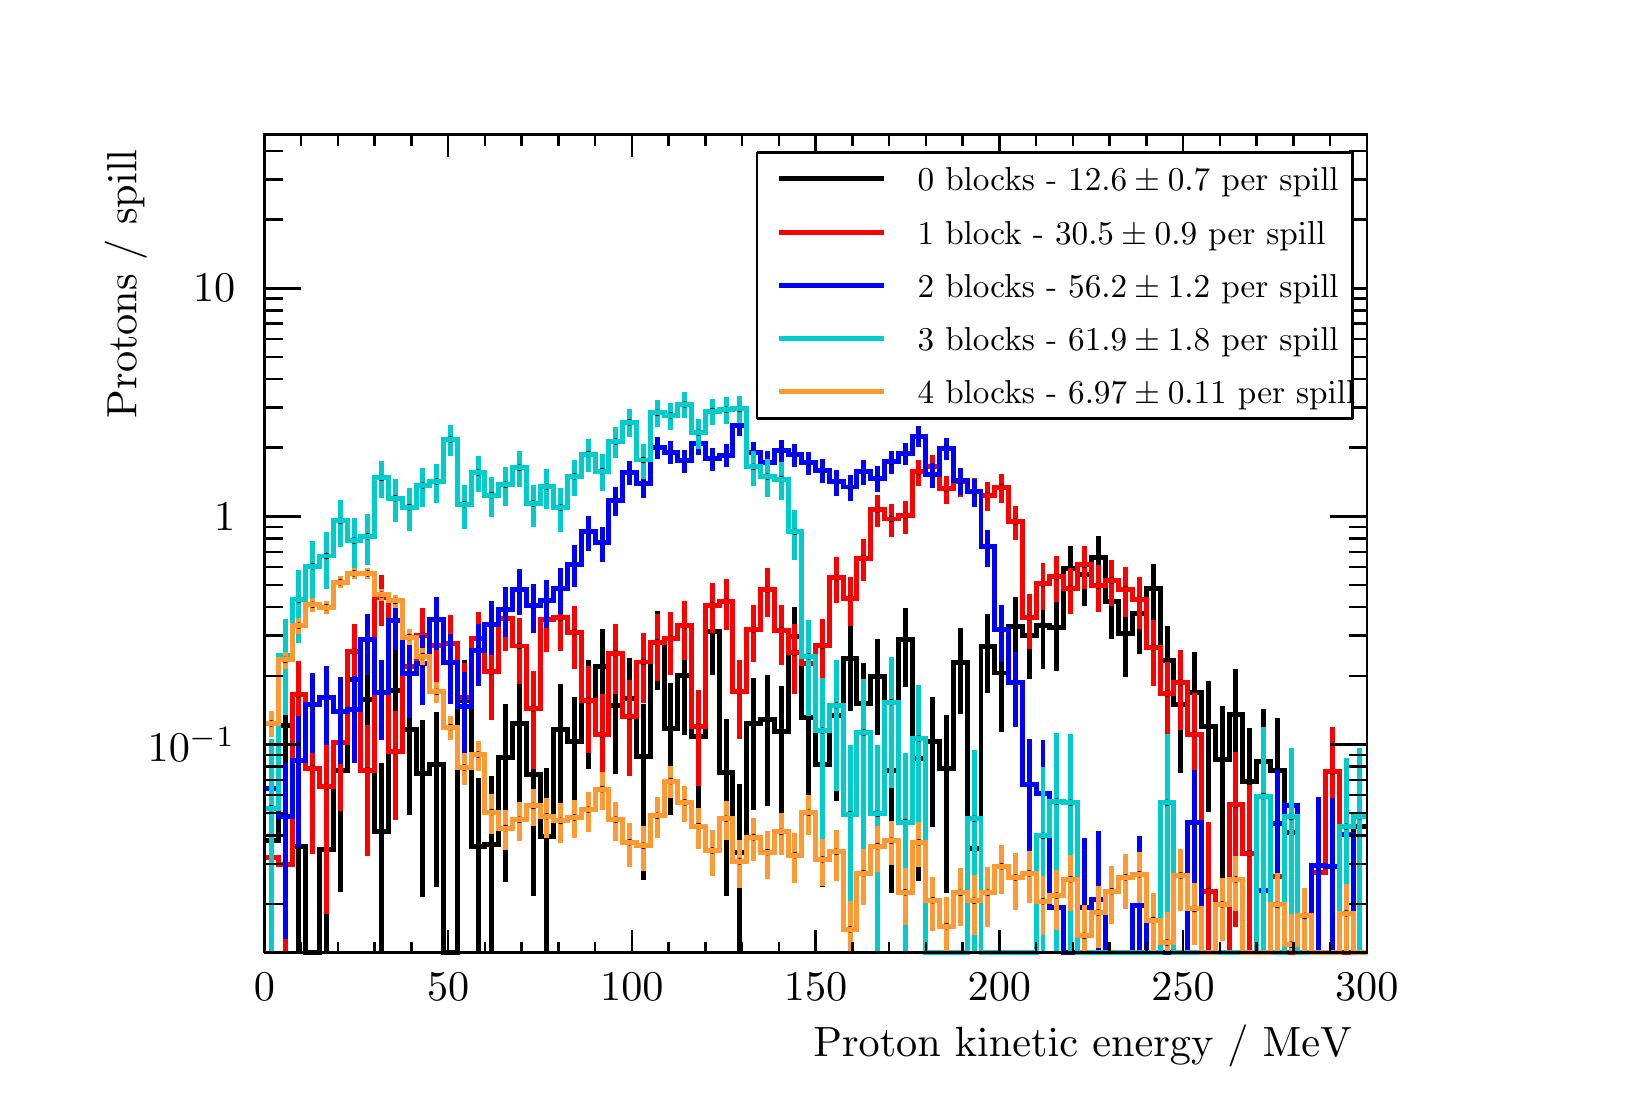
\begin{tikzpicture}
\pgfdeclareplotmark{cross} {
\pgfpathmoveto{\pgfpoint{-0.3\pgfplotmarksize}{\pgfplotmarksize}}
\pgfpathlineto{\pgfpoint{+0.3\pgfplotmarksize}{\pgfplotmarksize}}
\pgfpathlineto{\pgfpoint{+0.3\pgfplotmarksize}{0.3\pgfplotmarksize}}
\pgfpathlineto{\pgfpoint{+1\pgfplotmarksize}{0.3\pgfplotmarksize}}
\pgfpathlineto{\pgfpoint{+1\pgfplotmarksize}{-0.3\pgfplotmarksize}}
\pgfpathlineto{\pgfpoint{+0.3\pgfplotmarksize}{-0.3\pgfplotmarksize}}
\pgfpathlineto{\pgfpoint{+0.3\pgfplotmarksize}{-1.\pgfplotmarksize}}
\pgfpathlineto{\pgfpoint{-0.3\pgfplotmarksize}{-1.\pgfplotmarksize}}
\pgfpathlineto{\pgfpoint{-0.3\pgfplotmarksize}{-0.3\pgfplotmarksize}}
\pgfpathlineto{\pgfpoint{-1.\pgfplotmarksize}{-0.3\pgfplotmarksize}}
\pgfpathlineto{\pgfpoint{-1.\pgfplotmarksize}{0.3\pgfplotmarksize}}
\pgfpathlineto{\pgfpoint{-0.3\pgfplotmarksize}{0.3\pgfplotmarksize}}
\pgfpathclose
\pgfusepathqstroke
}
\pgfdeclareplotmark{cross*} {
\pgfpathmoveto{\pgfpoint{-0.3\pgfplotmarksize}{\pgfplotmarksize}}
\pgfpathlineto{\pgfpoint{+0.3\pgfplotmarksize}{\pgfplotmarksize}}
\pgfpathlineto{\pgfpoint{+0.3\pgfplotmarksize}{0.3\pgfplotmarksize}}
\pgfpathlineto{\pgfpoint{+1\pgfplotmarksize}{0.3\pgfplotmarksize}}
\pgfpathlineto{\pgfpoint{+1\pgfplotmarksize}{-0.3\pgfplotmarksize}}
\pgfpathlineto{\pgfpoint{+0.3\pgfplotmarksize}{-0.3\pgfplotmarksize}}
\pgfpathlineto{\pgfpoint{+0.3\pgfplotmarksize}{-1.\pgfplotmarksize}}
\pgfpathlineto{\pgfpoint{-0.3\pgfplotmarksize}{-1.\pgfplotmarksize}}
\pgfpathlineto{\pgfpoint{-0.3\pgfplotmarksize}{-0.3\pgfplotmarksize}}
\pgfpathlineto{\pgfpoint{-1.\pgfplotmarksize}{-0.3\pgfplotmarksize}}
\pgfpathlineto{\pgfpoint{-1.\pgfplotmarksize}{0.3\pgfplotmarksize}}
\pgfpathlineto{\pgfpoint{-0.3\pgfplotmarksize}{0.3\pgfplotmarksize}}
\pgfpathclose
\pgfusepathqfillstroke
}
\pgfdeclareplotmark{newstar} {
\pgfpathmoveto{\pgfqpoint{0pt}{\pgfplotmarksize}}
\pgfpathlineto{\pgfqpointpolar{44}{0.5\pgfplotmarksize}}
\pgfpathlineto{\pgfqpointpolar{18}{\pgfplotmarksize}}
\pgfpathlineto{\pgfqpointpolar{-20}{0.5\pgfplotmarksize}}
\pgfpathlineto{\pgfqpointpolar{-54}{\pgfplotmarksize}}
\pgfpathlineto{\pgfqpointpolar{-90}{0.5\pgfplotmarksize}}
\pgfpathlineto{\pgfqpointpolar{234}{\pgfplotmarksize}}
\pgfpathlineto{\pgfqpointpolar{198}{0.5\pgfplotmarksize}}
\pgfpathlineto{\pgfqpointpolar{162}{\pgfplotmarksize}}
\pgfpathlineto{\pgfqpointpolar{134}{0.5\pgfplotmarksize}}
\pgfpathclose
\pgfusepathqstroke
}
\pgfdeclareplotmark{newstar*} {
\pgfpathmoveto{\pgfqpoint{0pt}{\pgfplotmarksize}}
\pgfpathlineto{\pgfqpointpolar{44}{0.5\pgfplotmarksize}}
\pgfpathlineto{\pgfqpointpolar{18}{\pgfplotmarksize}}
\pgfpathlineto{\pgfqpointpolar{-20}{0.5\pgfplotmarksize}}
\pgfpathlineto{\pgfqpointpolar{-54}{\pgfplotmarksize}}
\pgfpathlineto{\pgfqpointpolar{-90}{0.5\pgfplotmarksize}}
\pgfpathlineto{\pgfqpointpolar{234}{\pgfplotmarksize}}
\pgfpathlineto{\pgfqpointpolar{198}{0.5\pgfplotmarksize}}
\pgfpathlineto{\pgfqpointpolar{162}{\pgfplotmarksize}}
\pgfpathlineto{\pgfqpointpolar{134}{0.5\pgfplotmarksize}}
\pgfpathclose
\pgfusepathqfillstroke
}
\definecolor{c}{rgb}{1,1,1};
\draw [color=c, fill=c] (0,0) rectangle (20,13.4957);
\draw [color=c, fill=c] (3,1.75444) rectangle (17,12.1461);
\definecolor{c}{rgb}{0,0,0};
\draw [c,line width=0.9] (3,1.75444) -- (3,12.1461) -- (17,12.1461) -- (17,1.75444) -- (3,1.75444);
\definecolor{c}{rgb}{1,1,1};
\draw [color=c, fill=c] (3,1.75444) rectangle (17,12.1461);
\definecolor{c}{rgb}{0,0,0};
\draw [c,line width=0.9] (3,1.75444) -- (3,12.1461) -- (17,12.1461) -- (17,1.75444) -- (3,1.75444);
\draw [c,line width=0.9] (3,1.75444) -- (3.175,1.75444) -- (3.175,1.75444) -- (3.35,1.75444) -- (3.35,1.75444) -- (3.525,1.75444) -- (3.525,1.75444) -- (3.7,1.75444) -- (3.7,1.75444) -- (3.875,1.75444) -- (3.875,1.75444) -- (4.05,1.75444) --
 (4.05,1.75444) -- (4.225,1.75444) -- (4.225,1.75444) -- (4.4,1.75444) -- (4.4,1.75444) -- (4.575,1.75444) -- (4.575,1.75444) -- (4.75,1.75444) -- (4.75,1.75444) -- (4.925,1.75444) -- (4.925,1.75444) -- (5.1,1.75444) -- (5.1,1.75444) --
 (5.275,1.75444) -- (5.275,1.75444) -- (5.45,1.75444) -- (5.45,1.75444) -- (5.625,1.75444) -- (5.625,1.75444) -- (5.8,1.75444) -- (5.8,1.75444) -- (5.975,1.75444) -- (5.975,1.75444) -- (6.15,1.75444) -- (6.15,1.75444) -- (6.325,1.75444) --
 (6.325,1.75444) -- (6.5,1.75444) -- (6.5,1.75444) -- (6.675,1.75444) -- (6.675,1.75444) -- (6.85,1.75444) -- (6.85,1.75444) -- (7.025,1.75444) -- (7.025,1.75444) -- (7.2,1.75444) -- (7.2,1.75444) -- (7.375,1.75444) -- (7.375,1.75444) --
 (7.55,1.75444) -- (7.55,1.75444) -- (7.725,1.75444) -- (7.725,1.75444) -- (7.9,1.75444) -- (7.9,1.75444) -- (8.075,1.75444) -- (8.075,1.75444) -- (8.25,1.75444) -- (8.25,1.75444) -- (8.425,1.75444) -- (8.425,1.75444) -- (8.6,1.75444) --
 (8.6,1.75444) -- (8.775,1.75444) -- (8.775,1.75444) -- (8.95,1.75444) -- (8.95,1.75444) -- (9.125,1.75444) -- (9.125,1.75444) -- (9.3,1.75444) -- (9.3,1.75444) -- (9.475,1.75444) -- (9.475,1.75444) -- (9.65,1.75444) -- (9.65,1.75444) --
 (9.825,1.75444) -- (9.825,1.75444) -- (10,1.75444) -- (10,1.75444) -- (10.175,1.75444) -- (10.175,1.75444) -- (10.35,1.75444) -- (10.35,1.75444) -- (10.525,1.75444) -- (10.525,1.75444) -- (10.7,1.75444) -- (10.7,1.75444) -- (10.875,1.75444) --
 (10.875,1.75444) -- (11.05,1.75444) -- (11.05,1.75444) -- (11.225,1.75444) -- (11.225,1.75444) -- (11.4,1.75444) -- (11.4,1.75444) -- (11.575,1.75444) -- (11.575,1.75444) -- (11.75,1.75444) -- (11.75,1.75444) -- (11.925,1.75444) -- (11.925,1.75444)
 -- (12.1,1.75444) -- (12.1,1.75444) -- (12.275,1.75444) -- (12.275,1.75444) -- (12.45,1.75444) -- (12.45,1.75444) -- (12.625,1.75444) -- (12.625,1.75444) -- (12.8,1.75444) -- (12.8,1.75444) -- (12.975,1.75444) -- (12.975,1.75444) -- (13.15,1.75444)
 -- (13.15,1.75444) -- (13.325,1.75444) -- (13.325,1.75444) -- (13.5,1.75444) -- (13.5,1.75444) -- (13.675,1.75444) -- (13.675,1.75444) -- (13.85,1.75444) -- (13.85,1.75444) -- (14.025,1.75444) -- (14.025,1.75444) -- (14.2,1.75444) -- (14.2,1.75444)
 -- (14.375,1.75444) -- (14.375,1.75444) -- (14.55,1.75444) -- (14.55,1.75444) -- (14.725,1.75444) -- (14.725,1.75444) -- (14.9,1.75444) -- (14.9,1.75444) -- (15.075,1.75444) -- (15.075,1.75444) -- (15.25,1.75444) -- (15.25,1.75444) --
 (15.425,1.75444) -- (15.425,1.75444) -- (15.6,1.75444) -- (15.6,1.75444) -- (15.775,1.75444) -- (15.775,1.75444) -- (15.95,1.75444) -- (15.95,1.75444) -- (16.125,1.75444) -- (16.125,1.75444) -- (16.3,1.75444) -- (16.3,1.75444) -- (16.475,1.75444) --
 (16.475,1.75444) -- (16.65,1.75444) -- (16.65,1.75444) -- (16.825,1.75444) -- (16.825,1.75444) -- (17,1.75444);
\draw [c,line width=0.9] (3,1.75444) -- (17,1.75444);
\draw [c,line width=0.9] (3,2.03785) -- (3,1.75444);
\draw [c,line width=0.9] (3.46667,1.89615) -- (3.46667,1.75444);
\draw [c,line width=0.9] (3.93333,1.89615) -- (3.93333,1.75444);
\draw [c,line width=0.9] (4.4,1.89615) -- (4.4,1.75444);
\draw [c,line width=0.9] (4.86667,1.89615) -- (4.86667,1.75444);
\draw [c,line width=0.9] (5.33333,2.03785) -- (5.33333,1.75444);
\draw [c,line width=0.9] (5.8,1.89615) -- (5.8,1.75444);
\draw [c,line width=0.9] (6.26667,1.89615) -- (6.26667,1.75444);
\draw [c,line width=0.9] (6.73333,1.89615) -- (6.73333,1.75444);
\draw [c,line width=0.9] (7.2,1.89615) -- (7.2,1.75444);
\draw [c,line width=0.9] (7.66667,2.03785) -- (7.66667,1.75444);
\draw [c,line width=0.9] (8.13333,1.89615) -- (8.13333,1.75444);
\draw [c,line width=0.9] (8.6,1.89615) -- (8.6,1.75444);
\draw [c,line width=0.9] (9.06667,1.89615) -- (9.06667,1.75444);
\draw [c,line width=0.9] (9.53333,1.89615) -- (9.53333,1.75444);
\draw [c,line width=0.9] (10,2.03785) -- (10,1.75444);
\draw [c,line width=0.9] (10.4667,1.89615) -- (10.4667,1.75444);
\draw [c,line width=0.9] (10.9333,1.89615) -- (10.9333,1.75444);
\draw [c,line width=0.9] (11.4,1.89615) -- (11.4,1.75444);
\draw [c,line width=0.9] (11.8667,1.89615) -- (11.8667,1.75444);
\draw [c,line width=0.9] (12.3333,2.03785) -- (12.3333,1.75444);
\draw [c,line width=0.9] (12.8,1.89615) -- (12.8,1.75444);
\draw [c,line width=0.9] (13.2667,1.89615) -- (13.2667,1.75444);
\draw [c,line width=0.9] (13.7333,1.89615) -- (13.7333,1.75444);
\draw [c,line width=0.9] (14.2,1.89615) -- (14.2,1.75444);
\draw [c,line width=0.9] (14.6667,2.03785) -- (14.6667,1.75444);
\draw [c,line width=0.9] (15.1333,1.89615) -- (15.1333,1.75444);
\draw [c,line width=0.9] (15.6,1.89615) -- (15.6,1.75444);
\draw [c,line width=0.9] (16.0667,1.89615) -- (16.0667,1.75444);
\draw [c,line width=0.9] (16.5333,1.89615) -- (16.5333,1.75444);
\draw [c,line width=0.9] (17,2.03785) -- (17,1.75444);
\draw [anchor=base] (3,1.14713) node[scale=1.52731, color=c, rotate=0]{0};
\draw [anchor=base] (5.33333,1.14713) node[scale=1.52731, color=c, rotate=0]{50};
\draw [anchor=base] (7.66667,1.14713) node[scale=1.52731, color=c, rotate=0]{100};
\draw [anchor=base] (10,1.14713) node[scale=1.52731, color=c, rotate=0]{150};
\draw [anchor=base] (12.3333,1.14713) node[scale=1.52731, color=c, rotate=0]{200};
\draw [anchor=base] (14.6667,1.14713) node[scale=1.52731, color=c, rotate=0]{250};
\draw [anchor=base] (17,1.14713) node[scale=1.52731, color=c, rotate=0]{300};
\draw [anchor= east] (17,0.566819) node[scale=1.52731, color=c, rotate=0]{ Proton kinetic energy / MeV};
\draw [c,line width=0.9] (3,12.1461) -- (17,12.1461);
\draw [c,line width=0.9] (3,11.8627) -- (3,12.1461);
\draw [c,line width=0.9] (3.46667,12.0044) -- (3.46667,12.1461);
\draw [c,line width=0.9] (3.93333,12.0044) -- (3.93333,12.1461);
\draw [c,line width=0.9] (4.4,12.0044) -- (4.4,12.1461);
\draw [c,line width=0.9] (4.86667,12.0044) -- (4.86667,12.1461);
\draw [c,line width=0.9] (5.33333,11.8627) -- (5.33333,12.1461);
\draw [c,line width=0.9] (5.8,12.0044) -- (5.8,12.1461);
\draw [c,line width=0.9] (6.26667,12.0044) -- (6.26667,12.1461);
\draw [c,line width=0.9] (6.73333,12.0044) -- (6.73333,12.1461);
\draw [c,line width=0.9] (7.2,12.0044) -- (7.2,12.1461);
\draw [c,line width=0.9] (7.66667,11.8627) -- (7.66667,12.1461);
\draw [c,line width=0.9] (8.13333,12.0044) -- (8.13333,12.1461);
\draw [c,line width=0.9] (8.6,12.0044) -- (8.6,12.1461);
\draw [c,line width=0.9] (9.06667,12.0044) -- (9.06667,12.1461);
\draw [c,line width=0.9] (9.53333,12.0044) -- (9.53333,12.1461);
\draw [c,line width=0.9] (10,11.8627) -- (10,12.1461);
\draw [c,line width=0.9] (10.4667,12.0044) -- (10.4667,12.1461);
\draw [c,line width=0.9] (10.9333,12.0044) -- (10.9333,12.1461);
\draw [c,line width=0.9] (11.4,12.0044) -- (11.4,12.1461);
\draw [c,line width=0.9] (11.8667,12.0044) -- (11.8667,12.1461);
\draw [c,line width=0.9] (12.3333,11.8627) -- (12.3333,12.1461);
\draw [c,line width=0.9] (12.8,12.0044) -- (12.8,12.1461);
\draw [c,line width=0.9] (13.2667,12.0044) -- (13.2667,12.1461);
\draw [c,line width=0.9] (13.7333,12.0044) -- (13.7333,12.1461);
\draw [c,line width=0.9] (14.2,12.0044) -- (14.2,12.1461);
\draw [c,line width=0.9] (14.6667,11.8627) -- (14.6667,12.1461);
\draw [c,line width=0.9] (15.1333,12.0044) -- (15.1333,12.1461);
\draw [c,line width=0.9] (15.6,12.0044) -- (15.6,12.1461);
\draw [c,line width=0.9] (16.0667,12.0044) -- (16.0667,12.1461);
\draw [c,line width=0.9] (16.5333,12.0044) -- (16.5333,12.1461);
\draw [c,line width=0.9] (17,11.8627) -- (17,12.1461);
\draw [c,line width=0.9] (3,1.75444) -- (3,12.1461);
\draw [c,line width=0.9] (3.231,2.37317) -- (3,2.37317);
\draw [c,line width=0.9] (3.231,2.88337) -- (3,2.88337);
\draw [c,line width=0.9] (3.231,3.24536) -- (3,3.24536);
\draw [c,line width=0.9] (3.231,3.52614) -- (3,3.52614);
\draw [c,line width=0.9] (3.231,3.75556) -- (3,3.75556);
\draw [c,line width=0.9] (3.231,3.94952) -- (3,3.94952);
\draw [c,line width=0.9] (3.231,4.11755) -- (3,4.11755);
\draw [c,line width=0.9] (3.231,4.26575) -- (3,4.26575);
\draw [c,line width=0.9] (3.462,4.39833) -- (3,4.39833);
\draw [anchor= east] (2.82,4.39833) node[scale=1.52731, color=c, rotate=0]{$10^{-1}$};
\draw [c,line width=0.9] (3.231,5.27052) -- (3,5.27052);
\draw [c,line width=0.9] (3.231,5.78071) -- (3,5.78071);
\draw [c,line width=0.9] (3.231,6.1427) -- (3,6.1427);
\draw [c,line width=0.9] (3.231,6.42348) -- (3,6.42348);
\draw [c,line width=0.9] (3.231,6.6529) -- (3,6.6529);
\draw [c,line width=0.9] (3.231,6.84687) -- (3,6.84687);
\draw [c,line width=0.9] (3.231,7.01489) -- (3,7.01489);
\draw [c,line width=0.9] (3.231,7.16309) -- (3,7.16309);
\draw [c,line width=0.9] (3.462,7.29567) -- (3,7.29567);
\draw [anchor= east] (2.82,7.29567) node[scale=1.52731, color=c, rotate=0]{1};
\draw [c,line width=0.9] (3.231,8.16786) -- (3,8.16786);
\draw [c,line width=0.9] (3.231,8.67805) -- (3,8.67805);
\draw [c,line width=0.9] (3.231,9.04004) -- (3,9.04004);
\draw [c,line width=0.9] (3.231,9.32082) -- (3,9.32082);
\draw [c,line width=0.9] (3.231,9.55024) -- (3,9.55024);
\draw [c,line width=0.9] (3.231,9.74421) -- (3,9.74421);
\draw [c,line width=0.9] (3.231,9.91223) -- (3,9.91223);
\draw [c,line width=0.9] (3.231,10.0604) -- (3,10.0604);
\draw [c,line width=0.9] (3.462,10.193) -- (3,10.193);
\draw [anchor= east] (2.82,10.193) node[scale=1.52731, color=c, rotate=0]{10};
\draw [c,line width=0.9] (3.231,11.0652) -- (3,11.0652);
\draw [c,line width=0.9] (3.231,11.5754) -- (3,11.5754);
\draw [c,line width=0.9] (3.231,11.9374) -- (3,11.9374);
\draw [anchor= east] (1.24,12.1461) node[scale=1.52731, color=c, rotate=90]{ Protons / spill};
\draw [c,line width=0.9] (17,1.75444) -- (17,12.1461);
\draw [c,line width=0.9] (16.769,2.37317) -- (17,2.37317);
\draw [c,line width=0.9] (16.769,2.88337) -- (17,2.88337);
\draw [c,line width=0.9] (16.769,3.24536) -- (17,3.24536);
\draw [c,line width=0.9] (16.769,3.52614) -- (17,3.52614);
\draw [c,line width=0.9] (16.769,3.75556) -- (17,3.75556);
\draw [c,line width=0.9] (16.769,3.94952) -- (17,3.94952);
\draw [c,line width=0.9] (16.769,4.11755) -- (17,4.11755);
\draw [c,line width=0.9] (16.769,4.26575) -- (17,4.26575);
\draw [c,line width=0.9] (16.538,4.39833) -- (17,4.39833);
\draw [c,line width=0.9] (16.769,5.27052) -- (17,5.27052);
\draw [c,line width=0.9] (16.769,5.78071) -- (17,5.78071);
\draw [c,line width=0.9] (16.769,6.1427) -- (17,6.1427);
\draw [c,line width=0.9] (16.769,6.42348) -- (17,6.42348);
\draw [c,line width=0.9] (16.769,6.6529) -- (17,6.6529);
\draw [c,line width=0.9] (16.769,6.84687) -- (17,6.84687);
\draw [c,line width=0.9] (16.769,7.01489) -- (17,7.01489);
\draw [c,line width=0.9] (16.769,7.16309) -- (17,7.16309);
\draw [c,line width=0.9] (16.538,7.29567) -- (17,7.29567);
\draw [c,line width=0.9] (16.769,8.16786) -- (17,8.16786);
\draw [c,line width=0.9] (16.769,8.67805) -- (17,8.67805);
\draw [c,line width=0.9] (16.769,9.04004) -- (17,9.04004);
\draw [c,line width=0.9] (16.769,9.32082) -- (17,9.32082);
\draw [c,line width=0.9] (16.769,9.55024) -- (17,9.55024);
\draw [c,line width=0.9] (16.769,9.74421) -- (17,9.74421);
\draw [c,line width=0.9] (16.769,9.91223) -- (17,9.91223);
\draw [c,line width=0.9] (16.769,10.0604) -- (17,10.0604);
\draw [c,line width=0.9] (16.538,10.193) -- (17,10.193);
\draw [c,line width=0.9] (16.769,11.0652) -- (17,11.0652);
\draw [c,line width=0.9] (16.769,11.5754) -- (17,11.5754);
\draw [c,line width=0.9] (16.769,11.9374) -- (17,11.9374);
\draw [c,line width=1.8] (3.0875,1.75444) -- (3.0875,3.18295);
\draw [c,line width=1.8] (3.0875,3.18295) -- (3.0875,4.05514);
\foreach \P in {(3.0875,3.18295)}{\draw[mark options={color=c,fill=c},mark size=2.402402pt,mark=*,mark size=1pt] plot coordinates {\P};}
\draw [c,line width=1.8] (3.2625,3.55287) -- (3.2625,4.63773);
\draw [c,line width=1.8] (3.2625,4.63773) -- (3.2625,5.21152);
\foreach \P in {(3.2625,4.63773)}{\draw[mark options={color=c,fill=c},mark size=2.402402pt,mark=*,mark size=1pt] plot coordinates {\P};}
\draw [c,line width=1.8] (3.4375,1.75444) -- (3.4375,3.10637);
\draw [c,line width=1.8] (3.4375,3.10637) -- (3.4375,3.97856);
\foreach \P in {(3.4375,3.10637)}{\draw[mark options={color=c,fill=c},mark size=2.402402pt,mark=*,mark size=1pt] plot coordinates {\P};}
\draw [c,line width=1.8] (3.7875,1.75444) -- (3.7875,3.06576);
\draw [c,line width=1.8] (3.7875,3.06576) -- (3.7875,3.93795);
\foreach \P in {(3.7875,3.06576)}{\draw[mark options={color=c,fill=c},mark size=2.402402pt,mark=*,mark size=1pt] plot coordinates {\P};}
\draw [c,line width=1.8] (3.9625,2.52015) -- (3.9625,4.07039);
\draw [c,line width=1.8] (3.9625,4.07039) -- (3.9625,4.74421);
\foreach \P in {(3.9625,4.07039)}{\draw[mark options={color=c,fill=c},mark size=2.402402pt,mark=*,mark size=1pt] plot coordinates {\P};}
\draw [c,line width=1.8] (4.1375,4.48291) -- (4.1375,5.22906);
\draw [c,line width=1.8] (4.1375,5.22906) -- (4.1375,5.69428);
\foreach \P in {(4.1375,5.22906)}{\draw[mark options={color=c,fill=c},mark size=2.402402pt,mark=*,mark size=1pt] plot coordinates {\P};}
\draw [c,line width=1.8] (4.3125,4.10056) -- (4.3125,4.9767);
\draw [c,line width=1.8] (4.3125,4.9767) -- (4.3125,5.48821);
\foreach \P in {(4.3125,4.9767)}{\draw[mark options={color=c,fill=c},mark size=2.402402pt,mark=*,mark size=1pt] plot coordinates {\P};}
\draw [c,line width=1.8] (4.4875,1.75444) -- (4.4875,3.28811);
\draw [c,line width=1.8] (4.4875,3.28811) -- (4.4875,4.1603);
\foreach \P in {(4.4875,3.28811)}{\draw[mark options={color=c,fill=c},mark size=2.402402pt,mark=*,mark size=1pt] plot coordinates {\P};}
\draw [c,line width=1.8] (4.6625,4.20578) -- (4.6625,5.08847);
\draw [c,line width=1.8] (4.6625,5.08847) -- (4.6625,5.60215);
\foreach \P in {(4.6625,5.08847)}{\draw[mark options={color=c,fill=c},mark size=2.402402pt,mark=*,mark size=1pt] plot coordinates {\P};}
\draw [c,line width=1.8] (4.8375,3.50132) -- (4.8375,4.58612);
\draw [c,line width=1.8] (4.8375,4.58612) -- (4.8375,5.15988);
\foreach \P in {(4.8375,4.58612)}{\draw[mark options={color=c,fill=c},mark size=2.402402pt,mark=*,mark size=1pt] plot coordinates {\P};}
\draw [c,line width=1.8] (5.0125,2.45676) -- (5.0125,4.03684);
\draw [c,line width=1.8] (5.0125,4.03684) -- (5.0125,4.71568);
\foreach \P in {(5.0125,4.03684)}{\draw[mark options={color=c,fill=c},mark size=2.402402pt,mark=*,mark size=1pt] plot coordinates {\P};}
\draw [c,line width=1.8] (5.1875,2.59094) -- (5.1875,4.13962);
\draw [c,line width=1.8] (5.1875,4.13962) -- (5.1875,4.81317);
\foreach \P in {(5.1875,4.13962)}{\draw[mark options={color=c,fill=c},mark size=2.402402pt,mark=*,mark size=1pt] plot coordinates {\P};}
\draw [c,line width=1.8] (5.5375,4.08207) -- (5.5375,4.96055);
\draw [c,line width=1.8] (5.5375,4.96055) -- (5.5375,5.47284);
\foreach \P in {(5.5375,4.96055)}{\draw[mark options={color=c,fill=c},mark size=2.402402pt,mark=*,mark size=1pt] plot coordinates {\P};}
\draw [c,line width=1.8] (5.7125,1.75444) -- (5.7125,3.10637);
\draw [c,line width=1.8] (5.7125,3.10637) -- (5.7125,3.97856);
\foreach \P in {(5.7125,3.10637)}{\draw[mark options={color=c,fill=c},mark size=2.402402pt,mark=*,mark size=1pt] plot coordinates {\P};}
\draw [c,line width=1.8] (5.8875,1.75444) -- (5.8875,3.12299);
\draw [c,line width=1.8] (5.8875,3.12299) -- (5.8875,3.99518);
\foreach \P in {(5.8875,3.12299)}{\draw[mark options={color=c,fill=c},mark size=2.402402pt,mark=*,mark size=1pt] plot coordinates {\P};}
\draw [c,line width=1.8] (6.0625,2.65183) -- (6.0625,4.23861);
\draw [c,line width=1.8] (6.0625,4.23861) -- (6.0625,4.91856);
\foreach \P in {(6.0625,4.23861)}{\draw[mark options={color=c,fill=c},mark size=2.402402pt,mark=*,mark size=1pt] plot coordinates {\P};}
\draw [c,line width=1.8] (6.2375,3.5631) -- (6.2375,4.66821);
\draw [c,line width=1.8] (6.2375,4.66821) -- (6.2375,5.24736);
\foreach \P in {(6.2375,4.66821)}{\draw[mark options={color=c,fill=c},mark size=2.402402pt,mark=*,mark size=1pt] plot coordinates {\P};}
\draw [c,line width=1.8] (6.4125,2.47529) -- (6.4125,4.02105);
\draw [c,line width=1.8] (6.4125,4.02105) -- (6.4125,4.69409);
\foreach \P in {(6.4125,4.02105)}{\draw[mark options={color=c,fill=c},mark size=2.402402pt,mark=*,mark size=1pt] plot coordinates {\P};}
\draw [c,line width=1.8] (6.5875,1.75444) -- (6.5875,3.2276);
\draw [c,line width=1.8] (6.5875,3.2276) -- (6.5875,4.09978);
\foreach \P in {(6.5875,3.2276)}{\draw[mark options={color=c,fill=c},mark size=2.402402pt,mark=*,mark size=1pt] plot coordinates {\P};}
\draw [c,line width=1.8] (6.7625,3.508) -- (6.7625,4.59415);
\draw [c,line width=1.8] (6.7625,4.59415) -- (6.7625,5.16828);
\foreach \P in {(6.7625,4.59415)}{\draw[mark options={color=c,fill=c},mark size=2.402402pt,mark=*,mark size=1pt] plot coordinates {\P};}
\draw [c,line width=1.8] (6.9375,3.35016) -- (6.9375,4.43436);
\draw [c,line width=1.8] (6.9375,4.43436) -- (6.9375,5.00798);
\foreach \P in {(6.9375,4.43436)}{\draw[mark options={color=c,fill=c},mark size=2.402402pt,mark=*,mark size=1pt] plot coordinates {\P};}
\draw [c,line width=1.8] (7.1125,4.08771) -- (7.1125,4.96133);
\draw [c,line width=1.8] (7.1125,4.96133) -- (7.1125,5.472);
\foreach \P in {(7.1125,4.96133)}{\draw[mark options={color=c,fill=c},mark size=2.402402pt,mark=*,mark size=1pt] plot coordinates {\P};}
\draw [c,line width=1.8] (7.2875,4.63904) -- (7.2875,5.39224);
\draw [c,line width=1.8] (7.2875,5.39224) -- (7.2875,5.86013);
\foreach \P in {(7.2875,5.39224)}{\draw[mark options={color=c,fill=c},mark size=2.402402pt,mark=*,mark size=1pt] plot coordinates {\P};}
\draw [c,line width=1.8] (7.4625,4.02007) -- (7.4625,4.89622);
\draw [c,line width=1.8] (7.4625,4.89622) -- (7.4625,5.40774);
\foreach \P in {(7.4625,4.89622)}{\draw[mark options={color=c,fill=c},mark size=2.402402pt,mark=*,mark size=1pt] plot coordinates {\P};}
\draw [c,line width=1.8] (7.6375,4.10362) -- (7.6375,4.98205);
\draw [c,line width=1.8] (7.6375,4.98205) -- (7.6375,5.49432);
\foreach \P in {(7.6375,4.98205)}{\draw[mark options={color=c,fill=c},mark size=2.402402pt,mark=*,mark size=1pt] plot coordinates {\P};}
\draw [c,line width=1.8] (7.8125,2.68096) -- (7.8125,4.2426);
\draw [c,line width=1.8] (7.8125,4.2426) -- (7.8125,4.91835);
\foreach \P in {(7.8125,4.2426)}{\draw[mark options={color=c,fill=c},mark size=2.402402pt,mark=*,mark size=1pt] plot coordinates {\P};}
\draw [c,line width=1.8] (7.9875,5.086) -- (7.9875,5.68848);
\draw [c,line width=1.8] (7.9875,5.68848) -- (7.9875,6.0942);
\foreach \P in {(7.9875,5.68848)}{\draw[mark options={color=c,fill=c},mark size=2.402402pt,mark=*,mark size=1pt] plot coordinates {\P};}
\draw [c,line width=1.8] (8.1625,3.50947) -- (8.1625,4.59939);
\draw [c,line width=1.8] (8.1625,4.59939) -- (8.1625,5.17453);
\foreach \P in {(8.1625,4.59939)}{\draw[mark options={color=c,fill=c},mark size=2.402402pt,mark=*,mark size=1pt] plot coordinates {\P};}
\draw [c,line width=1.8] (8.3375,4.5202) -- (8.3375,5.26948);
\draw [c,line width=1.8] (8.3375,5.26948) -- (8.3375,5.73588);
\foreach \P in {(8.3375,5.26948)}{\draw[mark options={color=c,fill=c},mark size=2.402402pt,mark=*,mark size=1pt] plot coordinates {\P};}
\draw [c,line width=1.8] (8.5125,3.40293) -- (8.5125,4.49452);
\draw [c,line width=1.8] (8.5125,4.49452) -- (8.5125,5.0701);
\foreach \P in {(8.5125,4.49452)}{\draw[mark options={color=c,fill=c},mark size=2.402402pt,mark=*,mark size=1pt] plot coordinates {\P};}
\draw [c,line width=1.8] (8.6875,5.27785) -- (8.6875,5.82921);
\draw [c,line width=1.8] (8.6875,5.82921) -- (8.6875,6.21128);
\foreach \P in {(8.6875,5.82921)}{\draw[mark options={color=c,fill=c},mark size=2.402402pt,mark=*,mark size=1pt] plot coordinates {\P};}
\draw [c,line width=1.8] (8.8625,2.48106) -- (8.8625,4.04327);
\draw [c,line width=1.8] (8.8625,4.04327) -- (8.8625,4.71911);
\foreach \P in {(8.8625,4.04327)}{\draw[mark options={color=c,fill=c},mark size=2.402402pt,mark=*,mark size=1pt] plot coordinates {\P};}
\draw [c,line width=1.8] (9.0375,1.75444) -- (9.0375,3.0303);
\draw [c,line width=1.8] (9.0375,3.0303) -- (9.0375,3.90248);
\foreach \P in {(9.0375,3.0303)}{\draw[mark options={color=c,fill=c},mark size=2.402402pt,mark=*,mark size=1pt] plot coordinates {\P};}
\draw [c,line width=1.8] (9.2125,3.56232) -- (9.2125,4.6645);
\draw [c,line width=1.8] (9.2125,4.6645) -- (9.2125,5.24289);
\foreach \P in {(9.2125,4.6645)}{\draw[mark options={color=c,fill=c},mark size=2.402402pt,mark=*,mark size=1pt] plot coordinates {\P};}
\draw [c,line width=1.8] (9.3875,3.62324) -- (9.3875,4.71202);
\draw [c,line width=1.8] (9.3875,4.71202) -- (9.3875,5.28686);
\foreach \P in {(9.3875,4.71202)}{\draw[mark options={color=c,fill=c},mark size=2.402402pt,mark=*,mark size=1pt] plot coordinates {\P};}
\draw [c,line width=1.8] (9.5625,3.48053) -- (9.5625,4.56491);
\draw [c,line width=1.8] (9.5625,4.56491) -- (9.5625,5.13857);
\foreach \P in {(9.5625,4.56491)}{\draw[mark options={color=c,fill=c},mark size=2.402402pt,mark=*,mark size=1pt] plot coordinates {\P};}
\draw [c,line width=1.8] (9.7375,5.2155) -- (9.7375,5.76587);
\draw [c,line width=1.8] (9.7375,5.76587) -- (9.7375,6.14748);
\foreach \P in {(9.7375,5.76587)}{\draw[mark options={color=c,fill=c},mark size=2.402402pt,mark=*,mark size=1pt] plot coordinates {\P};}
\draw [c,line width=1.8] (9.9125,3.65217) -- (9.9125,4.73914);
\draw [c,line width=1.8] (9.9125,4.73914) -- (9.9125,5.31349);
\foreach \P in {(9.9125,4.73914)}{\draw[mark options={color=c,fill=c},mark size=2.402402pt,mark=*,mark size=1pt] plot coordinates {\P};}
\draw [c,line width=1.8] (10.0875,2.59385) -- (10.0875,4.13923);
\draw [c,line width=1.8] (10.0875,4.13923) -- (10.0875,4.81222);
\foreach \P in {(10.0875,4.13923)}{\draw[mark options={color=c,fill=c},mark size=2.402402pt,mark=*,mark size=1pt] plot coordinates {\P};}
\draw [c,line width=1.8] (10.2625,3.67859) -- (10.2625,4.76501);
\draw [c,line width=1.8] (10.2625,4.76501) -- (10.2625,5.33921);
\foreach \P in {(10.2625,4.76501)}{\draw[mark options={color=c,fill=c},mark size=2.402402pt,mark=*,mark size=1pt] plot coordinates {\P};}
\draw [c,line width=1.8] (10.4375,4.82945) -- (10.4375,5.49185);
\draw [c,line width=1.8] (10.4375,5.49185) -- (10.4375,5.92355);
\foreach \P in {(10.4375,5.49185)}{\draw[mark options={color=c,fill=c},mark size=2.402402pt,mark=*,mark size=1pt] plot coordinates {\P};}
\draw [c,line width=1.8] (10.6125,4.05226) -- (10.6125,4.92582);
\draw [c,line width=1.8] (10.6125,4.92582) -- (10.6125,5.43647);
\foreach \P in {(10.6125,4.92582)}{\draw[mark options={color=c,fill=c},mark size=2.402402pt,mark=*,mark size=1pt] plot coordinates {\P};}
\draw [c,line width=1.8] (10.7875,4.52051) -- (10.7875,5.26759);
\draw [c,line width=1.8] (10.7875,5.26759) -- (10.7875,5.73316);
\foreach \P in {(10.7875,5.26759)}{\draw[mark options={color=c,fill=c},mark size=2.402402pt,mark=*,mark size=1pt] plot coordinates {\P};}
\draw [c,line width=1.8] (10.9625,2.51539) -- (10.9625,4.06762);
\draw [c,line width=1.8] (10.9625,4.06762) -- (10.9625,4.74178);
\foreach \P in {(10.9625,4.06762)}{\draw[mark options={color=c,fill=c},mark size=2.402402pt,mark=*,mark size=1pt] plot coordinates {\P};}
\draw [c,line width=1.8] (11.1375,5.12573) -- (11.1375,5.72725);
\draw [c,line width=1.8] (11.1375,5.72725) -- (11.1375,6.13253);
\foreach \P in {(11.1375,5.72725)}{\draw[mark options={color=c,fill=c},mark size=2.402402pt,mark=*,mark size=1pt] plot coordinates {\P};}
\draw [c,line width=1.8] (11.3125,2.66184) -- (11.3125,4.2184);
\draw [c,line width=1.8] (11.3125,4.2184) -- (11.3125,4.89329);
\foreach \P in {(11.3125,4.2184)}{\draw[mark options={color=c,fill=c},mark size=2.402402pt,mark=*,mark size=1pt] plot coordinates {\P};}
\draw [c,line width=1.8] (11.4875,3.35) -- (11.4875,4.43385);
\draw [c,line width=1.8] (11.4875,4.43385) -- (11.4875,5.00737);
\foreach \P in {(11.4875,4.43385)}{\draw[mark options={color=c,fill=c},mark size=2.402402pt,mark=*,mark size=1pt] plot coordinates {\P};}
\draw [c,line width=1.8] (11.6625,2.51319) -- (11.6625,4.0916);
\draw [c,line width=1.8] (11.6625,4.0916) -- (11.6625,4.77016);
\foreach \P in {(11.6625,4.0916)}{\draw[mark options={color=c,fill=c},mark size=2.402402pt,mark=*,mark size=1pt] plot coordinates {\P};}
\draw [c,line width=1.8] (11.8375,4.78202) -- (11.8375,5.44316);
\draw [c,line width=1.8] (11.8375,5.44316) -- (11.8375,5.87433);
\foreach \P in {(11.8375,5.44316)}{\draw[mark options={color=c,fill=c},mark size=2.402402pt,mark=*,mark size=1pt] plot coordinates {\P};}
\draw [c,line width=1.8] (12.0125,1.75444) -- (12.0125,3.07378);
\draw [c,line width=1.8] (12.0125,3.07378) -- (12.0125,3.94597);
\foreach \P in {(12.0125,3.07378)}{\draw[mark options={color=c,fill=c},mark size=2.402402pt,mark=*,mark size=1pt] plot coordinates {\P};}
\draw [c,line width=1.8] (12.1875,5.04715) -- (12.1875,5.64887);
\draw [c,line width=1.8] (12.1875,5.64887) -- (12.1875,6.05423);
\foreach \P in {(12.1875,5.64887)}{\draw[mark options={color=c,fill=c},mark size=2.402402pt,mark=*,mark size=1pt] plot coordinates {\P};}
\draw [c,line width=1.8] (12.3625,4.56059) -- (12.3625,5.30707);
\draw [c,line width=1.8] (12.3625,5.30707) -- (12.3625,5.77241);
\foreach \P in {(12.3625,5.30707)}{\draw[mark options={color=c,fill=c},mark size=2.402402pt,mark=*,mark size=1pt] plot coordinates {\P};}
\draw [c,line width=1.8] (12.5375,5.33975) -- (12.5375,5.89406);
\draw [c,line width=1.8] (12.5375,5.89406) -- (12.5375,6.27753);
\foreach \P in {(12.5375,5.89406)}{\draw[mark options={color=c,fill=c},mark size=2.402402pt,mark=*,mark size=1pt] plot coordinates {\P};}
\draw [c,line width=1.8] (12.7125,5.23534) -- (12.7125,5.78538);
\draw [c,line width=1.8] (12.7125,5.78538) -- (12.7125,6.16683);
\foreach \P in {(12.7125,5.78538)}{\draw[mark options={color=c,fill=c},mark size=2.402402pt,mark=*,mark size=1pt] plot coordinates {\P};}
\draw [c,line width=1.8] (12.8875,5.36179) -- (12.8875,5.91527);
\draw [c,line width=1.8] (12.8875,5.91527) -- (12.8875,6.29835);
\foreach \P in {(12.8875,5.91527)}{\draw[mark options={color=c,fill=c},mark size=2.402402pt,mark=*,mark size=1pt] plot coordinates {\P};}
\draw [c,line width=1.8] (13.0625,5.32976) -- (13.0625,5.88469);
\draw [c,line width=1.8] (13.0625,5.88469) -- (13.0625,6.26846);
\foreach \P in {(13.0625,5.88469)}{\draw[mark options={color=c,fill=c},mark size=2.402402pt,mark=*,mark size=1pt] plot coordinates {\P};}
\draw [c,line width=1.8] (13.2375,6.25118) -- (13.2375,6.62975);
\draw [c,line width=1.8] (13.2375,6.62975) -- (13.2375,6.92038);
\foreach \P in {(13.2375,6.62975)}{\draw[mark options={color=c,fill=c},mark size=2.402402pt,mark=*,mark size=1pt] plot coordinates {\P};}
\draw [c,line width=1.8] (13.4125,6.16038) -- (13.4125,6.5547);
\draw [c,line width=1.8] (13.4125,6.5547) -- (13.4125,6.85449);
\foreach \P in {(13.4125,6.5547)}{\draw[mark options={color=c,fill=c},mark size=2.402402pt,mark=*,mark size=1pt] plot coordinates {\P};}
\draw [c,line width=1.8] (13.5875,6.40701) -- (13.5875,6.77104);
\draw [c,line width=1.8] (13.5875,6.77104) -- (13.5875,7.05305);
\foreach \P in {(13.5875,6.77104)}{\draw[mark options={color=c,fill=c},mark size=2.402402pt,mark=*,mark size=1pt] plot coordinates {\P};}
\draw [c,line width=1.8] (13.7625,5.73749) -- (13.7625,6.21766);
\draw [c,line width=1.8] (13.7625,6.21766) -- (13.7625,6.56437);
\foreach \P in {(13.7625,6.21766)}{\draw[mark options={color=c,fill=c},mark size=2.402402pt,mark=*,mark size=1pt] plot coordinates {\P};}
\draw [c,line width=1.8] (13.9375,5.25983) -- (13.9375,5.81032);
\draw [c,line width=1.8] (13.9375,5.81032) -- (13.9375,6.19198);
\foreach \P in {(13.9375,5.81032)}{\draw[mark options={color=c,fill=c},mark size=2.402402pt,mark=*,mark size=1pt] plot coordinates {\P};}
\draw [c,line width=1.8] (14.1125,5.5422) -- (14.1125,6.05718);
\draw [c,line width=1.8] (14.1125,6.05718) -- (14.1125,6.42156);
\foreach \P in {(14.1125,6.05718)}{\draw[mark options={color=c,fill=c},mark size=2.402402pt,mark=*,mark size=1pt] plot coordinates {\P};}
\draw [c,line width=1.8] (14.2875,5.94502) -- (14.2875,6.37589);
\draw [c,line width=1.8] (14.2875,6.37589) -- (14.2875,6.69626);
\foreach \P in {(14.2875,6.37589)}{\draw[mark options={color=c,fill=c},mark size=2.402402pt,mark=*,mark size=1pt] plot coordinates {\P};}
\draw [c,line width=1.8] (14.4625,4.8014) -- (14.4625,5.4676);
\draw [c,line width=1.8] (14.4625,5.4676) -- (14.4625,5.90089);
\foreach \P in {(14.4625,5.4676)}{\draw[mark options={color=c,fill=c},mark size=2.402402pt,mark=*,mark size=1pt] plot coordinates {\P};}
\draw [c,line width=1.8] (14.6375,4.03789) -- (14.6375,4.91146);
\draw [c,line width=1.8] (14.6375,4.91146) -- (14.6375,5.42212);
\foreach \P in {(14.6375,4.91146)}{\draw[mark options={color=c,fill=c},mark size=2.402402pt,mark=*,mark size=1pt] plot coordinates {\P};}
\draw [c,line width=1.8] (14.8125,4.19097) -- (14.8125,5.06367);
\draw [c,line width=1.8] (14.8125,5.06367) -- (14.8125,5.57404);
\foreach \P in {(14.8125,5.06367)}{\draw[mark options={color=c,fill=c},mark size=2.402402pt,mark=*,mark size=1pt] plot coordinates {\P};}
\draw [c,line width=1.8] (14.9875,3.53994) -- (14.9875,4.63003);
\draw [c,line width=1.8] (14.9875,4.63003) -- (14.9875,5.20521);
\foreach \P in {(14.9875,4.63003)}{\draw[mark options={color=c,fill=c},mark size=2.402402pt,mark=*,mark size=1pt] plot coordinates {\P};}
\draw [c,line width=1.8] (15.1625,2.62222) -- (15.1625,4.211);
\draw [c,line width=1.8] (15.1625,4.211) -- (15.1625,4.89128);
\foreach \P in {(15.1625,4.211)}{\draw[mark options={color=c,fill=c},mark size=2.402402pt,mark=*,mark size=1pt] plot coordinates {\P};}
\draw [c,line width=1.8] (15.3375,3.68406) -- (15.3375,4.77618);
\draw [c,line width=1.8] (15.3375,4.77618) -- (15.3375,5.35191);
\foreach \P in {(15.3375,4.77618)}{\draw[mark options={color=c,fill=c},mark size=2.402402pt,mark=*,mark size=1pt] plot coordinates {\P};}
\draw [c,line width=1.8] (15.5125,2.38866) -- (15.5125,3.93476);
\draw [c,line width=1.8] (15.5125,3.93476) -- (15.5125,4.60787);
\foreach \P in {(15.5125,3.93476)}{\draw[mark options={color=c,fill=c},mark size=2.402402pt,mark=*,mark size=1pt] plot coordinates {\P};}
\draw [c,line width=1.8] (15.6875,2.6317) -- (15.6875,4.17844);
\draw [c,line width=1.8] (15.6875,4.17844) -- (15.6875,4.85166);
\foreach \P in {(15.6875,4.17844)}{\draw[mark options={color=c,fill=c},mark size=2.402402pt,mark=*,mark size=1pt] plot coordinates {\P};}
\draw [c,line width=1.8] (15.8625,2.50848) -- (15.8625,4.06256);
\draw [c,line width=1.8] (15.8625,4.06256) -- (15.8625,4.73703);
\foreach \P in {(15.8625,4.06256)}{\draw[mark options={color=c,fill=c},mark size=2.402402pt,mark=*,mark size=1pt] plot coordinates {\P};}
\draw [c,line width=1.8] (16.0375,1.75444) -- (16.0375,3.28335);
\draw [c,line width=1.8] (16.0375,3.28335) -- (16.0375,4.15554);
\foreach \P in {(16.0375,3.28335)}{\draw[mark options={color=c,fill=c},mark size=2.402402pt,mark=*,mark size=1pt] plot coordinates {\P};}
\draw [c,line width=1.8] (16.9125,1.75444) -- (16.9125,3.35168);
\draw [c,line width=1.8] (16.9125,3.35168) -- (16.9125,4.22387);
\foreach \P in {(16.9125,3.35168)}{\draw[mark options={color=c,fill=c},mark size=2.402402pt,mark=*,mark size=1pt] plot coordinates {\P};}
\draw [c,line width=1.8] (3,3.18295) -- (3.175,3.18295) -- (3.175,4.63773) -- (3.35,4.63773) -- (3.35,3.10637) -- (3.525,3.10637) -- (3.525,1.75444) -- (3.7,1.75444) -- (3.7,3.06576) -- (3.875,3.06576) -- (3.875,4.07039) -- (4.05,4.07039) --
 (4.05,5.22906) -- (4.225,5.22906) -- (4.225,4.9767) -- (4.4,4.9767) -- (4.4,3.28811) -- (4.575,3.28811) -- (4.575,5.08847) -- (4.75,5.08847) -- (4.75,4.58612) -- (4.925,4.58612) -- (4.925,4.03684) -- (5.1,4.03684) -- (5.1,4.13962) -- (5.275,4.13962)
 -- (5.275,1.75444) -- (5.45,1.75444) -- (5.45,4.96055) -- (5.625,4.96055) -- (5.625,3.10637) -- (5.8,3.10637) -- (5.8,3.12299) -- (5.975,3.12299) -- (5.975,4.23861) -- (6.15,4.23861) -- (6.15,4.66821) -- (6.325,4.66821) -- (6.325,4.02105) --
 (6.5,4.02105) -- (6.5,3.2276) -- (6.675,3.2276) -- (6.675,4.59415) -- (6.85,4.59415) -- (6.85,4.43436) -- (7.025,4.43436) -- (7.025,4.96133) -- (7.2,4.96133) -- (7.2,5.39224) -- (7.375,5.39224) -- (7.375,4.89622) -- (7.55,4.89622) -- (7.55,4.98205)
 -- (7.725,4.98205) -- (7.725,4.2426) -- (7.9,4.2426) -- (7.9,5.68848) -- (8.075,5.68848) -- (8.075,4.59939) -- (8.25,4.59939) -- (8.25,5.26948) -- (8.425,5.26948) -- (8.425,4.49452) -- (8.6,4.49452) -- (8.6,5.82921) -- (8.775,5.82921) --
 (8.775,4.04327) -- (8.95,4.04327) -- (8.95,3.0303) -- (9.125,3.0303) -- (9.125,4.6645) -- (9.3,4.6645) -- (9.3,4.71202) -- (9.475,4.71202) -- (9.475,4.56491) -- (9.65,4.56491) -- (9.65,5.76587) -- (9.825,5.76587) -- (9.825,4.73914) -- (10,4.73914)
 -- (10,4.13923) -- (10.175,4.13923) -- (10.175,4.76501) -- (10.35,4.76501) -- (10.35,5.49185) -- (10.525,5.49185) -- (10.525,4.92582) -- (10.7,4.92582) -- (10.7,5.26759) -- (10.875,5.26759) -- (10.875,4.06762) -- (11.05,4.06762) -- (11.05,5.72725)
 -- (11.225,5.72725) -- (11.225,4.2184) -- (11.4,4.2184) -- (11.4,4.43385) -- (11.575,4.43385) -- (11.575,4.0916) -- (11.75,4.0916) -- (11.75,5.44316) -- (11.925,5.44316) -- (11.925,3.07378) -- (12.1,3.07378) -- (12.1,5.64887) -- (12.275,5.64887) --
 (12.275,5.30707) -- (12.45,5.30707) -- (12.45,5.89406) -- (12.625,5.89406) -- (12.625,5.78538) -- (12.8,5.78538) -- (12.8,5.91527) -- (12.975,5.91527) -- (12.975,5.88469) -- (13.15,5.88469) -- (13.15,6.62975) -- (13.325,6.62975) -- (13.325,6.5547)
 -- (13.5,6.5547) -- (13.5,6.77104) -- (13.675,6.77104) -- (13.675,6.21766) -- (13.85,6.21766) -- (13.85,5.81032) -- (14.025,5.81032) -- (14.025,6.05718) -- (14.2,6.05718) -- (14.2,6.37589) -- (14.375,6.37589) -- (14.375,5.4676) -- (14.55,5.4676) --
 (14.55,4.91146) -- (14.725,4.91146) -- (14.725,5.06367) -- (14.9,5.06367) -- (14.9,4.63003) -- (15.075,4.63003) -- (15.075,4.211) -- (15.25,4.211) -- (15.25,4.77618) -- (15.425,4.77618) -- (15.425,3.93476) -- (15.6,3.93476) -- (15.6,4.17844) --
 (15.775,4.17844) -- (15.775,4.06256) -- (15.95,4.06256) -- (15.95,3.28335) -- (16.125,3.28335) -- (16.125,1.75444) -- (16.3,1.75444) -- (16.3,1.75444) -- (16.475,1.75444) -- (16.475,1.75444) -- (16.65,1.75444) -- (16.65,1.75444) -- (16.825,1.75444)
 -- (16.825,3.35168) -- (17,3.35168);
\definecolor{c}{rgb}{1,0,0};
\draw [c,line width=1.8] (3.0875,1.75444) -- (3.0875,2.96017);
\draw [c,line width=1.8] (3.0875,2.96017) -- (3.0875,3.83236);
\definecolor{c}{rgb}{0,0,0};
\foreach \P in {(3.0875,2.96017)}{\draw[mark options={color=c,fill=c},mark size=2.402402pt,mark=*,mark size=1pt] plot coordinates {\P};}
\definecolor{c}{rgb}{1,0,0};
\draw [c,line width=1.8] (3.2625,1.75444) -- (3.2625,2.87968);
\draw [c,line width=1.8] (3.2625,2.87968) -- (3.2625,3.75186);
\definecolor{c}{rgb}{0,0,0};
\foreach \P in {(3.2625,2.87968)}{\draw[mark options={color=c,fill=c},mark size=2.402402pt,mark=*,mark size=1pt] plot coordinates {\P};}
\definecolor{c}{rgb}{1,0,0};
\draw [c,line width=1.8] (3.4375,4.36906) -- (3.4375,5.03193);
\draw [c,line width=1.8] (3.4375,5.03193) -- (3.4375,5.46382);
\definecolor{c}{rgb}{0,0,0};
\foreach \P in {(3.4375,5.03193)}{\draw[mark options={color=c,fill=c},mark size=2.402402pt,mark=*,mark size=1pt] plot coordinates {\P};}
\definecolor{c}{rgb}{1,0,0};
\draw [c,line width=1.8] (3.6125,3.00662) -- (3.6125,4.09857);
\draw [c,line width=1.8] (3.6125,4.09857) -- (3.6125,4.67424);
\definecolor{c}{rgb}{0,0,0};
\foreach \P in {(3.6125,4.09857)}{\draw[mark options={color=c,fill=c},mark size=2.402402pt,mark=*,mark size=1pt] plot coordinates {\P};}
\definecolor{c}{rgb}{1,0,0};
\draw [c,line width=1.8] (3.7875,2.24945) -- (3.7875,3.85945);
\draw [c,line width=1.8] (3.7875,3.85945) -- (3.7875,4.54319);
\definecolor{c}{rgb}{0,0,0};
\foreach \P in {(3.7875,3.85945)}{\draw[mark options={color=c,fill=c},mark size=2.402402pt,mark=*,mark size=1pt] plot coordinates {\P};}
\definecolor{c}{rgb}{1,0,0};
\draw [c,line width=1.8] (3.9625,3.54822) -- (3.9625,4.42622);
\draw [c,line width=1.8] (3.9625,4.42622) -- (3.9625,4.93834);
\definecolor{c}{rgb}{0,0,0};
\foreach \P in {(3.9625,4.42622)}{\draw[mark options={color=c,fill=c},mark size=2.402402pt,mark=*,mark size=1pt] plot coordinates {\P};}
\definecolor{c}{rgb}{1,0,0};
\draw [c,line width=1.8] (4.1375,5.09511) -- (4.1375,5.57837);
\draw [c,line width=1.8] (4.1375,5.57837) -- (4.1375,5.92667);
\definecolor{c}{rgb}{0,0,0};
\foreach \P in {(4.1375,5.57837)}{\draw[mark options={color=c,fill=c},mark size=2.402402pt,mark=*,mark size=1pt] plot coordinates {\P};}
\definecolor{c}{rgb}{1,0,0};
\draw [c,line width=1.8] (4.3125,2.98368) -- (4.3125,4.07212);
\draw [c,line width=1.8] (4.3125,4.07212) -- (4.3125,4.64687);
\definecolor{c}{rgb}{0,0,0};
\foreach \P in {(4.3125,4.07212)}{\draw[mark options={color=c,fill=c},mark size=2.402402pt,mark=*,mark size=1pt] plot coordinates {\P};}
\definecolor{c}{rgb}{1,0,0};
\draw [c,line width=1.8] (4.4875,5.90066) -- (4.4875,6.26881);
\draw [c,line width=1.8] (4.4875,6.26881) -- (4.4875,6.55327);
\definecolor{c}{rgb}{0,0,0};
\foreach \P in {(4.4875,6.26881)}{\draw[mark options={color=c,fill=c},mark size=2.402402pt,mark=*,mark size=1pt] plot coordinates {\P};}
\definecolor{c}{rgb}{1,0,0};
\draw [c,line width=1.8] (4.6625,3.43426) -- (4.6625,4.3104);
\draw [c,line width=1.8] (4.6625,4.3104) -- (4.6625,4.82191);
\definecolor{c}{rgb}{0,0,0};
\foreach \P in {(4.6625,4.3104)}{\draw[mark options={color=c,fill=c},mark size=2.402402pt,mark=*,mark size=1pt] plot coordinates {\P};}
\definecolor{c}{rgb}{1,0,0};
\draw [c,line width=1.8] (4.8375,4.87662) -- (4.8375,5.39278);
\draw [c,line width=1.8] (4.8375,5.39278) -- (4.8375,5.75775);
\definecolor{c}{rgb}{0,0,0};
\foreach \P in {(4.8375,5.39278)}{\draw[mark options={color=c,fill=c},mark size=2.402402pt,mark=*,mark size=1pt] plot coordinates {\P};}
\definecolor{c}{rgb}{1,0,0};
\draw [c,line width=1.8] (5.0125,5.29215) -- (5.0125,5.78218);
\draw [c,line width=1.8] (5.0125,5.78218) -- (5.0125,6.13396);
\definecolor{c}{rgb}{0,0,0};
\foreach \P in {(5.0125,5.78218)}{\draw[mark options={color=c,fill=c},mark size=2.402402pt,mark=*,mark size=1pt] plot coordinates {\P};}
\definecolor{c}{rgb}{1,0,0};
\draw [c,line width=1.8] (5.1875,5.17338) -- (5.1875,5.65433);
\draw [c,line width=1.8] (5.1875,5.65433) -- (5.1875,6.00143);
\definecolor{c}{rgb}{0,0,0};
\foreach \P in {(5.1875,5.65433)}{\draw[mark options={color=c,fill=c},mark size=2.402402pt,mark=*,mark size=1pt] plot coordinates {\P};}
\definecolor{c}{rgb}{1,0,0};
\draw [c,line width=1.8] (5.3625,5.1997) -- (5.3625,5.68733);
\draw [c,line width=1.8] (5.3625,5.68733) -- (5.3625,6.03787);
\definecolor{c}{rgb}{0,0,0};
\foreach \P in {(5.3625,5.68733)}{\draw[mark options={color=c,fill=c},mark size=2.402402pt,mark=*,mark size=1pt] plot coordinates {\P};}
\definecolor{c}{rgb}{1,0,0};
\draw [c,line width=1.8] (5.5375,4.31548) -- (5.5375,4.99663);
\draw [c,line width=1.8] (5.5375,4.99663) -- (5.5375,5.43611);
\definecolor{c}{rgb}{0,0,0};
\foreach \P in {(5.5375,4.99663)}{\draw[mark options={color=c,fill=c},mark size=2.402402pt,mark=*,mark size=1pt] plot coordinates {\P};}
\definecolor{c}{rgb}{1,0,0};
\draw [c,line width=1.8] (5.7125,5.28742) -- (5.7125,5.74537);
\draw [c,line width=1.8] (5.7125,5.74537) -- (5.7125,6.08039);
\definecolor{c}{rgb}{0,0,0};
\foreach \P in {(5.7125,5.74537)}{\draw[mark options={color=c,fill=c},mark size=2.402402pt,mark=*,mark size=1pt] plot coordinates {\P};}
\definecolor{c}{rgb}{1,0,0};
\draw [c,line width=1.8] (5.8875,4.71321) -- (5.8875,5.32263);
\draw [c,line width=1.8] (5.8875,5.32263) -- (5.8875,5.73144);
\definecolor{c}{rgb}{0,0,0};
\foreach \P in {(5.8875,5.32263)}{\draw[mark options={color=c,fill=c},mark size=2.402402pt,mark=*,mark size=1pt] plot coordinates {\P};}
\definecolor{c}{rgb}{1,0,0};
\draw [c,line width=1.8] (6.0625,5.58562) -- (6.0625,6.00347);
\draw [c,line width=1.8] (6.0625,6.00347) -- (6.0625,6.31661);
\definecolor{c}{rgb}{0,0,0};
\foreach \P in {(6.0625,6.00347)}{\draw[mark options={color=c,fill=c},mark size=2.402402pt,mark=*,mark size=1pt] plot coordinates {\P};}
\definecolor{c}{rgb}{1,0,0};
\draw [c,line width=1.8] (6.2375,5.16289) -- (6.2375,5.64999);
\draw [c,line width=1.8] (6.2375,5.64999) -- (6.2375,6.00027);
\definecolor{c}{rgb}{0,0,0};
\foreach \P in {(6.2375,5.64999)}{\draw[mark options={color=c,fill=c},mark size=2.402402pt,mark=*,mark size=1pt] plot coordinates {\P};}
\definecolor{c}{rgb}{1,0,0};
\draw [c,line width=1.8] (6.4125,4.09069) -- (6.4125,4.85632);
\draw [c,line width=1.8] (6.4125,4.85632) -- (6.4125,5.32889);
\definecolor{c}{rgb}{0,0,0};
\foreach \P in {(6.4125,4.85632)}{\draw[mark options={color=c,fill=c},mark size=2.402402pt,mark=*,mark size=1pt] plot coordinates {\P};}
\definecolor{c}{rgb}{1,0,0};
\draw [c,line width=1.8] (6.5875,5.57371) -- (6.5875,5.99132);
\draw [c,line width=1.8] (6.5875,5.99132) -- (6.5875,6.30433);
\definecolor{c}{rgb}{0,0,0};
\foreach \P in {(6.5875,5.99132)}{\draw[mark options={color=c,fill=c},mark size=2.402402pt,mark=*,mark size=1pt] plot coordinates {\P};}
\definecolor{c}{rgb}{1,0,0};
\draw [c,line width=1.8] (6.7625,5.5922) -- (6.7625,6.00751);
\draw [c,line width=1.8] (6.7625,6.00751) -- (6.7625,6.31923);
\definecolor{c}{rgb}{0,0,0};
\foreach \P in {(6.7625,6.00751)}{\draw[mark options={color=c,fill=c},mark size=2.402402pt,mark=*,mark size=1pt] plot coordinates {\P};}
\definecolor{c}{rgb}{1,0,0};
\draw [c,line width=1.8] (6.9375,5.36135) -- (6.9375,5.82461);
\draw [c,line width=1.8] (6.9375,5.82461) -- (6.9375,6.16246);
\definecolor{c}{rgb}{0,0,0};
\foreach \P in {(6.9375,5.82461)}{\draw[mark options={color=c,fill=c},mark size=2.402402pt,mark=*,mark size=1pt] plot coordinates {\P};}
\definecolor{c}{rgb}{1,0,0};
\draw [c,line width=1.8] (7.1125,4.29366) -- (7.1125,4.96091);
\draw [c,line width=1.8] (7.1125,4.96091) -- (7.1125,5.39463);
\definecolor{c}{rgb}{0,0,0};
\foreach \P in {(7.1125,4.96091)}{\draw[mark options={color=c,fill=c},mark size=2.402402pt,mark=*,mark size=1pt] plot coordinates {\P};}
\definecolor{c}{rgb}{1,0,0};
\draw [c,line width=1.8] (7.2875,3.63606) -- (7.2875,4.52312);
\draw [c,line width=1.8] (7.2875,4.52312) -- (7.2875,5.03824);
\definecolor{c}{rgb}{0,0,0};
\foreach \P in {(7.2875,4.52312)}{\draw[mark options={color=c,fill=c},mark size=2.402402pt,mark=*,mark size=1pt] plot coordinates {\P};}
\definecolor{c}{rgb}{1,0,0};
\draw [c,line width=1.8] (7.4625,5.04034) -- (7.4625,5.56059);
\draw [c,line width=1.8] (7.4625,5.56059) -- (7.4625,5.92758);
\definecolor{c}{rgb}{0,0,0};
\foreach \P in {(7.4625,5.56059)}{\draw[mark options={color=c,fill=c},mark size=2.402402pt,mark=*,mark size=1pt] plot coordinates {\P};}
\definecolor{c}{rgb}{1,0,0};
\draw [c,line width=1.8] (7.6375,4.00224) -- (7.6375,4.75005);
\draw [c,line width=1.8] (7.6375,4.75005) -- (7.6375,5.2159);
\definecolor{c}{rgb}{0,0,0};
\foreach \P in {(7.6375,4.75005)}{\draw[mark options={color=c,fill=c},mark size=2.402402pt,mark=*,mark size=1pt] plot coordinates {\P};}
\definecolor{c}{rgb}{1,0,0};
\draw [c,line width=1.8] (7.8125,4.93172) -- (7.8125,5.44683);
\draw [c,line width=1.8] (7.8125,5.44683) -- (7.8125,5.81126);
\definecolor{c}{rgb}{0,0,0};
\foreach \P in {(7.8125,5.44683)}{\draw[mark options={color=c,fill=c},mark size=2.402402pt,mark=*,mark size=1pt] plot coordinates {\P};}
\definecolor{c}{rgb}{1,0,0};
\draw [c,line width=1.8] (7.9875,5.20784) -- (7.9875,5.69877);
\draw [c,line width=1.8] (7.9875,5.69877) -- (7.9875,6.05102);
\definecolor{c}{rgb}{0,0,0};
\foreach \P in {(7.9875,5.69877)}{\draw[mark options={color=c,fill=c},mark size=2.402402pt,mark=*,mark size=1pt] plot coordinates {\P};}
\definecolor{c}{rgb}{1,0,0};
\draw [c,line width=1.8] (8.1625,5.28112) -- (8.1625,5.74389);
\draw [c,line width=1.8] (8.1625,5.74389) -- (8.1625,6.08148);
\definecolor{c}{rgb}{0,0,0};
\foreach \P in {(8.1625,5.74389)}{\draw[mark options={color=c,fill=c},mark size=2.402402pt,mark=*,mark size=1pt] plot coordinates {\P};}
\definecolor{c}{rgb}{1,0,0};
\draw [c,line width=1.8] (8.3375,5.47463) -- (8.3375,5.90609);
\draw [c,line width=1.8] (8.3375,5.90609) -- (8.3375,6.22678);
\definecolor{c}{rgb}{0,0,0};
\foreach \P in {(8.3375,5.90609)}{\draw[mark options={color=c,fill=c},mark size=2.402402pt,mark=*,mark size=1pt] plot coordinates {\P};}
\definecolor{c}{rgb}{1,0,0};
\draw [c,line width=1.8] (8.5125,3.87497) -- (8.5125,4.62873);
\draw [c,line width=1.8] (8.5125,4.62873) -- (8.5125,5.09683);
\definecolor{c}{rgb}{0,0,0};
\foreach \P in {(8.5125,4.62873)}{\draw[mark options={color=c,fill=c},mark size=2.402402pt,mark=*,mark size=1pt] plot coordinates {\P};}
\definecolor{c}{rgb}{1,0,0};
\draw [c,line width=1.8] (8.6875,5.81598) -- (8.6875,6.16857);
\draw [c,line width=1.8] (8.6875,6.16857) -- (8.6875,6.44367);
\definecolor{c}{rgb}{0,0,0};
\foreach \P in {(8.6875,6.16857)}{\draw[mark options={color=c,fill=c},mark size=2.402402pt,mark=*,mark size=1pt] plot coordinates {\P};}
\definecolor{c}{rgb}{1,0,0};
\draw [c,line width=1.8] (8.8625,5.85213) -- (8.8625,6.2174);
\draw [c,line width=1.8] (8.8625,6.2174) -- (8.8625,6.50015);
\definecolor{c}{rgb}{0,0,0};
\foreach \P in {(8.8625,6.2174)}{\draw[mark options={color=c,fill=c},mark size=2.402402pt,mark=*,mark size=1pt] plot coordinates {\P};}
\definecolor{c}{rgb}{1,0,0};
\draw [c,line width=1.8] (9.0375,4.46678) -- (9.0375,5.0694);
\draw [c,line width=1.8] (9.0375,5.0694) -- (9.0375,5.47518);
\definecolor{c}{rgb}{0,0,0};
\foreach \P in {(9.0375,5.0694)}{\draw[mark options={color=c,fill=c},mark size=2.402402pt,mark=*,mark size=1pt] plot coordinates {\P};}
\definecolor{c}{rgb}{1,0,0};
\draw [c,line width=1.8] (9.2125,5.44684) -- (9.2125,5.85899);
\draw [c,line width=1.8] (9.2125,5.85899) -- (9.2125,6.16893);
\definecolor{c}{rgb}{0,0,0};
\foreach \P in {(9.2125,5.85899)}{\draw[mark options={color=c,fill=c},mark size=2.402402pt,mark=*,mark size=1pt] plot coordinates {\P};}
\definecolor{c}{rgb}{1,0,0};
\draw [c,line width=1.8] (9.3875,6.0238) -- (9.3875,6.36825);
\draw [c,line width=1.8] (9.3875,6.36825) -- (9.3875,6.63839);
\definecolor{c}{rgb}{0,0,0};
\foreach \P in {(9.3875,6.36825)}{\draw[mark options={color=c,fill=c},mark size=2.402402pt,mark=*,mark size=1pt] plot coordinates {\P};}
\definecolor{c}{rgb}{1,0,0};
\draw [c,line width=1.8] (9.5625,5.4117) -- (9.5625,5.84984);
\draw [c,line width=1.8] (9.5625,5.84984) -- (9.5625,6.1742);
\definecolor{c}{rgb}{0,0,0};
\foreach \P in {(9.5625,5.84984)}{\draw[mark options={color=c,fill=c},mark size=2.402402pt,mark=*,mark size=1pt] plot coordinates {\P};}
\definecolor{c}{rgb}{1,0,0};
\draw [c,line width=1.8] (9.7375,5.04358) -- (9.7375,5.56139);
\draw [c,line width=1.8] (9.7375,5.56139) -- (9.7375,5.92716);
\definecolor{c}{rgb}{0,0,0};
\foreach \P in {(9.7375,5.56139)}{\draw[mark options={color=c,fill=c},mark size=2.402402pt,mark=*,mark size=1pt] plot coordinates {\P};}
\definecolor{c}{rgb}{1,0,0};
\draw [c,line width=1.8] (9.9125,4.87046) -- (9.9125,5.43121);
\draw [c,line width=1.8] (9.9125,5.43121) -- (9.9125,5.81774);
\definecolor{c}{rgb}{0,0,0};
\foreach \P in {(9.9125,5.43121)}{\draw[mark options={color=c,fill=c},mark size=2.402402pt,mark=*,mark size=1pt] plot coordinates {\P};}
\definecolor{c}{rgb}{1,0,0};
\draw [c,line width=1.8] (10.0875,5.16862) -- (10.0875,5.65071);
\draw [c,line width=1.8] (10.0875,5.65071) -- (10.0875,5.99841);
\definecolor{c}{rgb}{0,0,0};
\foreach \P in {(10.0875,5.65071)}{\draw[mark options={color=c,fill=c},mark size=2.402402pt,mark=*,mark size=1pt] plot coordinates {\P};}
\definecolor{c}{rgb}{1,0,0};
\draw [c,line width=1.8] (10.2625,6.19717) -- (10.2625,6.52048);
\draw [c,line width=1.8] (10.2625,6.52048) -- (10.2625,6.77746);
\definecolor{c}{rgb}{0,0,0};
\foreach \P in {(10.2625,6.52048)}{\draw[mark options={color=c,fill=c},mark size=2.402402pt,mark=*,mark size=1pt] plot coordinates {\P};}
\definecolor{c}{rgb}{1,0,0};
\draw [c,line width=1.8] (10.4375,5.90018) -- (10.4375,6.25247);
\draw [c,line width=1.8] (10.4375,6.25247) -- (10.4375,6.52739);
\definecolor{c}{rgb}{0,0,0};
\foreach \P in {(10.4375,6.25247)}{\draw[mark options={color=c,fill=c},mark size=2.402402pt,mark=*,mark size=1pt] plot coordinates {\P};}
\definecolor{c}{rgb}{1,0,0};
\draw [c,line width=1.8] (10.6125,6.47013) -- (10.6125,6.76453);
\draw [c,line width=1.8] (10.6125,6.76453) -- (10.6125,7.00294);
\definecolor{c}{rgb}{0,0,0};
\foreach \P in {(10.6125,6.76453)}{\draw[mark options={color=c,fill=c},mark size=2.402402pt,mark=*,mark size=1pt] plot coordinates {\P};}
\definecolor{c}{rgb}{1,0,0};
\draw [c,line width=1.8] (10.7875,7.16162) -- (10.7875,7.38444);
\draw [c,line width=1.8] (10.7875,7.38444) -- (10.7875,7.57367);
\definecolor{c}{rgb}{0,0,0};
\foreach \P in {(10.7875,7.38444)}{\draw[mark options={color=c,fill=c},mark size=2.402402pt,mark=*,mark size=1pt] plot coordinates {\P};}
\definecolor{c}{rgb}{1,0,0};
\draw [c,line width=1.8] (10.9625,7.03436) -- (10.9625,7.26272);
\draw [c,line width=1.8] (10.9625,7.26272) -- (10.9625,7.45594);
\definecolor{c}{rgb}{0,0,0};
\foreach \P in {(10.9625,7.26272)}{\draw[mark options={color=c,fill=c},mark size=2.402402pt,mark=*,mark size=1pt] plot coordinates {\P};}
\definecolor{c}{rgb}{1,0,0};
\draw [c,line width=1.8] (11.1375,7.07581) -- (11.1375,7.30405);
\draw [c,line width=1.8] (11.1375,7.30405) -- (11.1375,7.49718);
\definecolor{c}{rgb}{0,0,0};
\foreach \P in {(11.1375,7.30405)}{\draw[mark options={color=c,fill=c},mark size=2.402402pt,mark=*,mark size=1pt] plot coordinates {\P};}
\definecolor{c}{rgb}{1,0,0};
\draw [c,line width=1.8] (11.3125,7.68238) -- (11.3125,7.86039);
\draw [c,line width=1.8] (11.3125,7.86039) -- (11.3125,8.0163);
\definecolor{c}{rgb}{0,0,0};
\foreach \P in {(11.3125,7.86039)}{\draw[mark options={color=c,fill=c},mark size=2.402402pt,mark=*,mark size=1pt] plot coordinates {\P};}
\definecolor{c}{rgb}{1,0,0};
\draw [c,line width=1.8] (11.4875,7.75017) -- (11.4875,7.9266);
\draw [c,line width=1.8] (11.4875,7.9266) -- (11.4875,8.0813);
\definecolor{c}{rgb}{0,0,0};
\foreach \P in {(11.4875,7.9266)}{\draw[mark options={color=c,fill=c},mark size=2.402402pt,mark=*,mark size=1pt] plot coordinates {\P};}
\definecolor{c}{rgb}{1,0,0};
\draw [c,line width=1.8] (11.6625,7.45432) -- (11.6625,7.64638);
\draw [c,line width=1.8] (11.6625,7.64638) -- (11.6625,7.81297);
\definecolor{c}{rgb}{0,0,0};
\foreach \P in {(11.6625,7.64638)}{\draw[mark options={color=c,fill=c},mark size=2.402402pt,mark=*,mark size=1pt] plot coordinates {\P};}
\definecolor{c}{rgb}{1,0,0};
\draw [c,line width=1.8] (11.8375,7.54635) -- (11.8375,7.73644);
\draw [c,line width=1.8] (11.8375,7.73644) -- (11.8375,7.90155);
\definecolor{c}{rgb}{0,0,0};
\foreach \P in {(11.8375,7.73644)}{\draw[mark options={color=c,fill=c},mark size=2.402402pt,mark=*,mark size=1pt] plot coordinates {\P};}
\definecolor{c}{rgb}{1,0,0};
\draw [c,line width=1.8] (12.0125,7.41888) -- (12.0125,7.61314);
\draw [c,line width=1.8] (12.0125,7.61314) -- (12.0125,7.78138);
\definecolor{c}{rgb}{0,0,0};
\foreach \P in {(12.0125,7.61314)}{\draw[mark options={color=c,fill=c},mark size=2.402402pt,mark=*,mark size=1pt] plot coordinates {\P};}
\definecolor{c}{rgb}{1,0,0};
\draw [c,line width=1.8] (12.1875,7.36297) -- (12.1875,7.56475);
\draw [c,line width=1.8] (12.1875,7.56475) -- (12.1875,7.7386);
\definecolor{c}{rgb}{0,0,0};
\foreach \P in {(12.1875,7.56475)}{\draw[mark options={color=c,fill=c},mark size=2.402402pt,mark=*,mark size=1pt] plot coordinates {\P};}
\definecolor{c}{rgb}{1,0,0};
\draw [c,line width=1.8] (12.3625,7.46684) -- (12.3625,7.66548);
\draw [c,line width=1.8] (12.3625,7.66548) -- (12.3625,7.83699);
\definecolor{c}{rgb}{0,0,0};
\foreach \P in {(12.3625,7.66548)}{\draw[mark options={color=c,fill=c},mark size=2.402402pt,mark=*,mark size=1pt] plot coordinates {\P};}
\definecolor{c}{rgb}{1,0,0};
\draw [c,line width=1.8] (12.5375,6.99416) -- (12.5375,7.22928);
\draw [c,line width=1.8] (12.5375,7.22928) -- (12.5375,7.42731);
\definecolor{c}{rgb}{0,0,0};
\foreach \P in {(12.5375,7.22928)}{\draw[mark options={color=c,fill=c},mark size=2.402402pt,mark=*,mark size=1pt] plot coordinates {\P};}
\definecolor{c}{rgb}{1,0,0};
\draw [c,line width=1.8] (12.7125,5.61687) -- (12.7125,6.01096);
\draw [c,line width=1.8] (12.7125,6.01096) -- (12.7125,6.31062);
\definecolor{c}{rgb}{0,0,0};
\foreach \P in {(12.7125,6.01096)}{\draw[mark options={color=c,fill=c},mark size=2.402402pt,mark=*,mark size=1pt] plot coordinates {\P};}
\definecolor{c}{rgb}{1,0,0};
\draw [c,line width=1.8] (12.8875,6.1075) -- (12.8875,6.43964);
\draw [c,line width=1.8] (12.8875,6.43964) -- (12.8875,6.70217);
\definecolor{c}{rgb}{0,0,0};
\foreach \P in {(12.8875,6.43964)}{\draw[mark options={color=c,fill=c},mark size=2.402402pt,mark=*,mark size=1pt] plot coordinates {\P};}
\definecolor{c}{rgb}{1,0,0};
\draw [c,line width=1.8] (13.0625,6.20421) -- (13.0625,6.52925);
\draw [c,line width=1.8] (13.0625,6.52925) -- (13.0625,6.78733);
\definecolor{c}{rgb}{0,0,0};
\foreach \P in {(13.0625,6.52925)}{\draw[mark options={color=c,fill=c},mark size=2.402402pt,mark=*,mark size=1pt] plot coordinates {\P};}
\definecolor{c}{rgb}{1,0,0};
\draw [c,line width=1.8] (13.2375,6.05262) -- (13.2375,6.38426);
\draw [c,line width=1.8] (13.2375,6.38426) -- (13.2375,6.64647);
\definecolor{c}{rgb}{0,0,0};
\foreach \P in {(13.2375,6.38426)}{\draw[mark options={color=c,fill=c},mark size=2.402402pt,mark=*,mark size=1pt] plot coordinates {\P};}
\definecolor{c}{rgb}{1,0,0};
\draw [c,line width=1.8] (13.4125,6.37505) -- (13.4125,6.68024);
\draw [c,line width=1.8] (13.4125,6.68024) -- (13.4125,6.92568);
\definecolor{c}{rgb}{0,0,0};
\foreach \P in {(13.4125,6.68024)}{\draw[mark options={color=c,fill=c},mark size=2.402402pt,mark=*,mark size=1pt] plot coordinates {\P};}
\definecolor{c}{rgb}{1,0,0};
\draw [c,line width=1.8] (13.5875,6.08224) -- (13.5875,6.41417);
\draw [c,line width=1.8] (13.5875,6.41417) -- (13.5875,6.67657);
\definecolor{c}{rgb}{0,0,0};
\foreach \P in {(13.5875,6.41417)}{\draw[mark options={color=c,fill=c},mark size=2.402402pt,mark=*,mark size=1pt] plot coordinates {\P};}
\definecolor{c}{rgb}{1,0,0};
\draw [c,line width=1.8] (13.7625,6.15999) -- (13.7625,6.48206);
\draw [c,line width=1.8] (13.7625,6.48206) -- (13.7625,6.73826);
\definecolor{c}{rgb}{0,0,0};
\foreach \P in {(13.7625,6.48206)}{\draw[mark options={color=c,fill=c},mark size=2.402402pt,mark=*,mark size=1pt] plot coordinates {\P};}
\definecolor{c}{rgb}{1,0,0};
\draw [c,line width=1.8] (13.9375,6.01791) -- (13.9375,6.37155);
\draw [c,line width=1.8] (13.9375,6.37155) -- (13.9375,6.64729);
\definecolor{c}{rgb}{0,0,0};
\foreach \P in {(13.9375,6.37155)}{\draw[mark options={color=c,fill=c},mark size=2.402402pt,mark=*,mark size=1pt] plot coordinates {\P};}
\definecolor{c}{rgb}{1,0,0};
\draw [c,line width=1.8] (14.1125,5.8704) -- (14.1125,6.23986);
\draw [c,line width=1.8] (14.1125,6.23986) -- (14.1125,6.5251);
\definecolor{c}{rgb}{0,0,0};
\foreach \P in {(14.1125,6.23986)}{\draw[mark options={color=c,fill=c},mark size=2.402402pt,mark=*,mark size=1pt] plot coordinates {\P};}
\definecolor{c}{rgb}{1,0,0};
\draw [c,line width=1.8] (14.2875,5.14513) -- (14.2875,5.63042);
\draw [c,line width=1.8] (14.2875,5.63042) -- (14.2875,5.97976);
\definecolor{c}{rgb}{0,0,0};
\foreach \P in {(14.2875,5.63042)}{\draw[mark options={color=c,fill=c},mark size=2.402402pt,mark=*,mark size=1pt] plot coordinates {\P};}
\definecolor{c}{rgb}{1,0,0};
\draw [c,line width=1.8] (14.4625,4.4445) -- (14.4625,5.04561);
\draw [c,line width=1.8] (14.4625,5.04561) -- (14.4625,5.45071);
\definecolor{c}{rgb}{0,0,0};
\foreach \P in {(14.4625,5.04561)}{\draw[mark options={color=c,fill=c},mark size=2.402402pt,mark=*,mark size=1pt] plot coordinates {\P};}
\definecolor{c}{rgb}{1,0,0};
\draw [c,line width=1.8] (14.6375,4.57784) -- (14.6375,5.18697);
\draw [c,line width=1.8] (14.6375,5.18697) -- (14.6375,5.59565);
\definecolor{c}{rgb}{0,0,0};
\foreach \P in {(14.6375,5.18697)}{\draw[mark options={color=c,fill=c},mark size=2.402402pt,mark=*,mark size=1pt] plot coordinates {\P};}
\definecolor{c}{rgb}{1,0,0};
\draw [c,line width=1.8] (14.8125,3.61939) -- (14.8125,4.52632);
\draw [c,line width=1.8] (14.8125,4.52632) -- (14.8125,5.04789);
\definecolor{c}{rgb}{0,0,0};
\foreach \P in {(14.8125,4.52632)}{\draw[mark options={color=c,fill=c},mark size=2.402402pt,mark=*,mark size=1pt] plot coordinates {\P};}
\definecolor{c}{rgb}{1,0,0};
\draw [c,line width=1.8] (14.9875,1.75444) -- (14.9875,2.5382);
\draw [c,line width=1.8] (14.9875,2.5382) -- (14.9875,3.41039);
\definecolor{c}{rgb}{0,0,0};
\foreach \P in {(14.9875,2.5382)}{\draw[mark options={color=c,fill=c},mark size=2.402402pt,mark=*,mark size=1pt] plot coordinates {\P};}
\definecolor{c}{rgb}{1,0,0};
\draw [c,line width=1.8] (15.3375,2.07664) -- (15.3375,3.6314);
\draw [c,line width=1.8] (15.3375,3.6314) -- (15.3375,4.30599);
\definecolor{c}{rgb}{0,0,0};
\foreach \P in {(15.3375,3.6314)}{\draw[mark options={color=c,fill=c},mark size=2.402402pt,mark=*,mark size=1pt] plot coordinates {\P};}
\definecolor{c}{rgb}{1,0,0};
\draw [c,line width=1.8] (15.5125,1.75444) -- (15.5125,3.01866);
\draw [c,line width=1.8] (15.5125,3.01866) -- (15.5125,3.89084);
\definecolor{c}{rgb}{0,0,0};
\foreach \P in {(15.5125,3.01866)}{\draw[mark options={color=c,fill=c},mark size=2.402402pt,mark=*,mark size=1pt] plot coordinates {\P};}
\definecolor{c}{rgb}{1,0,0};
\draw [c,line width=1.8] (15.8625,1.75444) -- (15.8625,2.71758);
\draw [c,line width=1.8] (15.8625,2.71758) -- (15.8625,3.58977);
\definecolor{c}{rgb}{0,0,0};
\foreach \P in {(15.8625,2.71758)}{\draw[mark options={color=c,fill=c},mark size=2.402402pt,mark=*,mark size=1pt] plot coordinates {\P};}
\definecolor{c}{rgb}{1,0,0};
\draw [c,line width=1.8] (16.3875,1.75444) -- (16.3875,2.77679);
\draw [c,line width=1.8] (16.3875,2.77679) -- (16.3875,3.64897);
\definecolor{c}{rgb}{0,0,0};
\foreach \P in {(16.3875,2.77679)}{\draw[mark options={color=c,fill=c},mark size=2.402402pt,mark=*,mark size=1pt] plot coordinates {\P};}
\definecolor{c}{rgb}{1,0,0};
\draw [c,line width=1.8] (16.5625,2.96287) -- (16.5625,4.05097);
\draw [c,line width=1.8] (16.5625,4.05097) -- (16.5625,4.62563);
\definecolor{c}{rgb}{0,0,0};
\foreach \P in {(16.5625,4.05097)}{\draw[mark options={color=c,fill=c},mark size=2.402402pt,mark=*,mark size=1pt] plot coordinates {\P};}
\definecolor{c}{rgb}{1,0,0};
\draw [c,line width=1.8] (3,2.96017) -- (3.175,2.96017) -- (3.175,2.87968) -- (3.35,2.87968) -- (3.35,5.03193) -- (3.525,5.03193) -- (3.525,4.09857) -- (3.7,4.09857) -- (3.7,3.85945) -- (3.875,3.85945) -- (3.875,4.42622) -- (4.05,4.42622) --
 (4.05,5.57837) -- (4.225,5.57837) -- (4.225,4.07212) -- (4.4,4.07212) -- (4.4,6.26881) -- (4.575,6.26881) -- (4.575,4.3104) -- (4.75,4.3104) -- (4.75,5.39278) -- (4.925,5.39278) -- (4.925,5.78218) -- (5.1,5.78218) -- (5.1,5.65433) -- (5.275,5.65433)
 -- (5.275,5.68733) -- (5.45,5.68733) -- (5.45,4.99663) -- (5.625,4.99663) -- (5.625,5.74537) -- (5.8,5.74537) -- (5.8,5.32263) -- (5.975,5.32263) -- (5.975,6.00347) -- (6.15,6.00347) -- (6.15,5.64999) -- (6.325,5.64999) -- (6.325,4.85632) --
 (6.5,4.85632) -- (6.5,5.99132) -- (6.675,5.99132) -- (6.675,6.00751) -- (6.85,6.00751) -- (6.85,5.82461) -- (7.025,5.82461) -- (7.025,4.96091) -- (7.2,4.96091) -- (7.2,4.52312) -- (7.375,4.52312) -- (7.375,5.56059) -- (7.55,5.56059) --
 (7.55,4.75005) -- (7.725,4.75005) -- (7.725,5.44683) -- (7.9,5.44683) -- (7.9,5.69877) -- (8.075,5.69877) -- (8.075,5.74389) -- (8.25,5.74389) -- (8.25,5.90609) -- (8.425,5.90609) -- (8.425,4.62873) -- (8.6,4.62873) -- (8.6,6.16857) --
 (8.775,6.16857) -- (8.775,6.2174) -- (8.95,6.2174) -- (8.95,5.0694) -- (9.125,5.0694) -- (9.125,5.85899) -- (9.3,5.85899) -- (9.3,6.36825) -- (9.475,6.36825) -- (9.475,5.84984) -- (9.65,5.84984) -- (9.65,5.56139) -- (9.825,5.56139) --
 (9.825,5.43121) -- (10,5.43121) -- (10,5.65071) -- (10.175,5.65071) -- (10.175,6.52048) -- (10.35,6.52048) -- (10.35,6.25247) -- (10.525,6.25247) -- (10.525,6.76453) -- (10.7,6.76453) -- (10.7,7.38444) -- (10.875,7.38444) -- (10.875,7.26272) --
 (11.05,7.26272) -- (11.05,7.30405) -- (11.225,7.30405) -- (11.225,7.86039) -- (11.4,7.86039) -- (11.4,7.9266) -- (11.575,7.9266) -- (11.575,7.64638) -- (11.75,7.64638) -- (11.75,7.73644) -- (11.925,7.73644) -- (11.925,7.61314) -- (12.1,7.61314) --
 (12.1,7.56475) -- (12.275,7.56475) -- (12.275,7.66548) -- (12.45,7.66548) -- (12.45,7.22928) -- (12.625,7.22928) -- (12.625,6.01096) -- (12.8,6.01096) -- (12.8,6.43964) -- (12.975,6.43964) -- (12.975,6.52925) -- (13.15,6.52925) -- (13.15,6.38426) --
 (13.325,6.38426) -- (13.325,6.68024) -- (13.5,6.68024) -- (13.5,6.41417) -- (13.675,6.41417) -- (13.675,6.48206) -- (13.85,6.48206) -- (13.85,6.37155) -- (14.025,6.37155) -- (14.025,6.23986) -- (14.2,6.23986) -- (14.2,5.63042) -- (14.375,5.63042) --
 (14.375,5.04561) -- (14.55,5.04561) -- (14.55,5.18697) -- (14.725,5.18697) -- (14.725,4.52632) -- (14.9,4.52632) -- (14.9,2.5382) -- (15.075,2.5382) -- (15.075,1.75444) -- (15.25,1.75444) -- (15.25,3.6314) -- (15.425,3.6314) -- (15.425,3.01866) --
 (15.6,3.01866) -- (15.6,1.75444) -- (15.775,1.75444) -- (15.775,2.71758) -- (15.95,2.71758) -- (15.95,1.75444) -- (16.125,1.75444) -- (16.125,1.75444) -- (16.3,1.75444) -- (16.3,2.77679) -- (16.475,2.77679) -- (16.475,4.05097) -- (16.65,4.05097) --
 (16.65,1.75444) -- (16.825,1.75444) -- (16.825,1.75444) -- (17,1.75444);
\definecolor{c}{rgb}{0,0,1};
\draw [c,line width=1.8] (3.0875,2.73853) -- (3.0875,3.83589);
\draw [c,line width=1.8] (3.0875,3.83589) -- (3.0875,4.413);
\definecolor{c}{rgb}{0,0,0};
\foreach \P in {(3.0875,3.83589)}{\draw[mark options={color=c,fill=c},mark size=2.402402pt,mark=*,mark size=1pt] plot coordinates {\P};}
\definecolor{c}{rgb}{0,0,1};
\draw [c,line width=1.8] (3.2625,1.93331) -- (3.2625,3.48838);
\draw [c,line width=1.8] (3.2625,3.48838) -- (3.2625,4.16302);
\definecolor{c}{rgb}{0,0,0};
\foreach \P in {(3.2625,3.48838)}{\draw[mark options={color=c,fill=c},mark size=2.402402pt,mark=*,mark size=1pt] plot coordinates {\P};}
\definecolor{c}{rgb}{0,0,1};
\draw [c,line width=1.8] (3.4375,3.09524) -- (3.4375,4.19066);
\draw [c,line width=1.8] (3.4375,4.19066) -- (3.4375,4.76726);
\definecolor{c}{rgb}{0,0,0};
\foreach \P in {(3.4375,4.19066)}{\draw[mark options={color=c,fill=c},mark size=2.402402pt,mark=*,mark size=1pt] plot coordinates {\P};}
\definecolor{c}{rgb}{0,0,1};
\draw [c,line width=1.8] (3.6125,4.29735) -- (3.6125,4.90457);
\draw [c,line width=1.8] (3.6125,4.90457) -- (3.6125,5.31241);
\definecolor{c}{rgb}{0,0,0};
\foreach \P in {(3.6125,4.90457)}{\draw[mark options={color=c,fill=c},mark size=2.402402pt,mark=*,mark size=1pt] plot coordinates {\P};}
\definecolor{c}{rgb}{0,0,1};
\draw [c,line width=1.8] (3.7875,4.38987) -- (3.7875,4.99103);
\draw [c,line width=1.8] (3.7875,4.99103) -- (3.7875,5.39615);
\definecolor{c}{rgb}{0,0,0};
\foreach \P in {(3.7875,4.99103)}{\draw[mark options={color=c,fill=c},mark size=2.402402pt,mark=*,mark size=1pt] plot coordinates {\P};}
\definecolor{c}{rgb}{0,0,1};
\draw [c,line width=1.8] (3.9625,4.14602) -- (3.9625,4.81757);
\draw [c,line width=1.8] (3.9625,4.81757) -- (3.9625,5.25308);
\definecolor{c}{rgb}{0,0,0};
\foreach \P in {(3.9625,4.81757)}{\draw[mark options={color=c,fill=c},mark size=2.402402pt,mark=*,mark size=1pt] plot coordinates {\P};}
\definecolor{c}{rgb}{0,0,1};
\draw [c,line width=1.8] (4.1375,4.16785) -- (4.1375,4.83934);
\draw [c,line width=1.8] (4.1375,4.83934) -- (4.1375,5.27484);
\definecolor{c}{rgb}{0,0,0};
\foreach \P in {(4.1375,4.83934)}{\draw[mark options={color=c,fill=c},mark size=2.402402pt,mark=*,mark size=1pt] plot coordinates {\P};}
\definecolor{c}{rgb}{0,0,1};
\draw [c,line width=1.8] (4.3125,5.28765) -- (4.3125,5.72626);
\draw [c,line width=1.8] (4.3125,5.72626) -- (4.3125,6.05088);
\definecolor{c}{rgb}{0,0,0};
\foreach \P in {(4.3125,5.72626)}{\draw[mark options={color=c,fill=c},mark size=2.402402pt,mark=*,mark size=1pt] plot coordinates {\P};}
\definecolor{c}{rgb}{0,0,1};
\draw [c,line width=1.8] (4.4875,4.45353) -- (4.4875,5.06004);
\draw [c,line width=1.8] (4.4875,5.06004) -- (4.4875,5.46756);
\definecolor{c}{rgb}{0,0,0};
\foreach \P in {(4.4875,5.06004)}{\draw[mark options={color=c,fill=c},mark size=2.402402pt,mark=*,mark size=1pt] plot coordinates {\P};}
\definecolor{c}{rgb}{0,0,1};
\draw [c,line width=1.8] (4.6625,5.59296) -- (4.6625,5.97564);
\draw [c,line width=1.8] (4.6625,5.97564) -- (4.6625,6.26867);
\definecolor{c}{rgb}{0,0,0};
\foreach \P in {(4.6625,5.97564)}{\draw[mark options={color=c,fill=c},mark size=2.402402pt,mark=*,mark size=1pt] plot coordinates {\P};}
\definecolor{c}{rgb}{0,0,1};
\draw [c,line width=1.8] (4.8375,4.73173) -- (4.8375,5.29685);
\draw [c,line width=1.8] (4.8375,5.29685) -- (4.8375,5.68542);
\definecolor{c}{rgb}{0,0,0};
\foreach \P in {(4.8375,5.29685)}{\draw[mark options={color=c,fill=c},mark size=2.402402pt,mark=*,mark size=1pt] plot coordinates {\P};}
\definecolor{c}{rgb}{0,0,1};
\draw [c,line width=1.8] (5.0125,4.8988) -- (5.0125,5.42179);
\draw [c,line width=1.8] (5.0125,5.42179) -- (5.0125,5.79013);
\definecolor{c}{rgb}{0,0,0};
\foreach \P in {(5.0125,5.42179)}{\draw[mark options={color=c,fill=c},mark size=2.402402pt,mark=*,mark size=1pt] plot coordinates {\P};}
\definecolor{c}{rgb}{0,0,1};
\draw [c,line width=1.8] (5.1875,5.60266) -- (5.1875,5.98232);
\draw [c,line width=1.8] (5.1875,5.98232) -- (5.1875,6.27359);
\definecolor{c}{rgb}{0,0,0};
\foreach \P in {(5.1875,5.98232)}{\draw[mark options={color=c,fill=c},mark size=2.402402pt,mark=*,mark size=1pt] plot coordinates {\P};}
\definecolor{c}{rgb}{0,0,1};
\draw [c,line width=1.8] (5.3625,4.91674) -- (5.3625,5.4349);
\draw [c,line width=1.8] (5.3625,5.4349) -- (5.3625,5.80085);
\definecolor{c}{rgb}{0,0,0};
\foreach \P in {(5.3625,5.4349)}{\draw[mark options={color=c,fill=c},mark size=2.402402pt,mark=*,mark size=1pt] plot coordinates {\P};}
\definecolor{c}{rgb}{0,0,1};
\draw [c,line width=1.8] (5.5375,4.21671) -- (5.5375,4.88623);
\draw [c,line width=1.8] (5.5375,4.88623) -- (5.5375,5.32091);
\definecolor{c}{rgb}{0,0,0};
\foreach \P in {(5.5375,4.88623)}{\draw[mark options={color=c,fill=c},mark size=2.402402pt,mark=*,mark size=1pt] plot coordinates {\P};}
\definecolor{c}{rgb}{0,0,1};
\draw [c,line width=1.8] (5.7125,5.14364) -- (5.7125,5.59701);
\draw [c,line width=1.8] (5.7125,5.59701) -- (5.7125,5.9296);
\definecolor{c}{rgb}{0,0,0};
\foreach \P in {(5.7125,5.59701)}{\draw[mark options={color=c,fill=c},mark size=2.402402pt,mark=*,mark size=1pt] plot coordinates {\P};}
\definecolor{c}{rgb}{0,0,1};
\draw [c,line width=1.8] (5.8875,5.5331) -- (5.8875,5.92159);
\draw [c,line width=1.8] (5.8875,5.92159) -- (5.8875,6.218);
\definecolor{c}{rgb}{0,0,0};
\foreach \P in {(5.8875,5.92159)}{\draw[mark options={color=c,fill=c},mark size=2.402402pt,mark=*,mark size=1pt] plot coordinates {\P};}
\definecolor{c}{rgb}{0,0,1};
\draw [c,line width=1.8] (6.0625,5.76258) -- (6.0625,6.11763);
\draw [c,line width=1.8] (6.0625,6.11763) -- (6.0625,6.39423);
\definecolor{c}{rgb}{0,0,0};
\foreach \P in {(6.0625,6.11763)}{\draw[mark options={color=c,fill=c},mark size=2.402402pt,mark=*,mark size=1pt] plot coordinates {\P};}
\definecolor{c}{rgb}{0,0,1};
\draw [c,line width=1.8] (6.2375,6.04568) -- (6.2375,6.3706);
\draw [c,line width=1.8] (6.2375,6.3706) -- (6.2375,6.6286);
\definecolor{c}{rgb}{0,0,0};
\foreach \P in {(6.2375,6.3706)}{\draw[mark options={color=c,fill=c},mark size=2.402402pt,mark=*,mark size=1pt] plot coordinates {\P};}
\definecolor{c}{rgb}{0,0,1};
\draw [c,line width=1.8] (6.4125,5.81023) -- (6.4125,6.16389);
\draw [c,line width=1.8] (6.4125,6.16389) -- (6.4125,6.43964);
\definecolor{c}{rgb}{0,0,0};
\foreach \P in {(6.4125,6.16389)}{\draw[mark options={color=c,fill=c},mark size=2.402402pt,mark=*,mark size=1pt] plot coordinates {\P};}
\definecolor{c}{rgb}{0,0,1};
\draw [c,line width=1.8] (6.5875,5.8792) -- (6.5875,6.22234);
\draw [c,line width=1.8] (6.5875,6.22234) -- (6.5875,6.49168);
\definecolor{c}{rgb}{0,0,0};
\foreach \P in {(6.5875,6.22234)}{\draw[mark options={color=c,fill=c},mark size=2.402402pt,mark=*,mark size=1pt] plot coordinates {\P};}
\definecolor{c}{rgb}{0,0,1};
\draw [c,line width=1.8] (6.7625,6.05463) -- (6.7625,6.38016);
\draw [c,line width=1.8] (6.7625,6.38016) -- (6.7625,6.63855);
\definecolor{c}{rgb}{0,0,0};
\foreach \P in {(6.7625,6.38016)}{\draw[mark options={color=c,fill=c},mark size=2.402402pt,mark=*,mark size=1pt] plot coordinates {\P};}
\definecolor{c}{rgb}{0,0,1};
\draw [c,line width=1.8] (6.9375,6.39711) -- (6.9375,6.69047);
\draw [c,line width=1.8] (6.9375,6.69047) -- (6.9375,6.92821);
\definecolor{c}{rgb}{0,0,0};
\foreach \P in {(6.9375,6.69047)}{\draw[mark options={color=c,fill=c},mark size=2.402402pt,mark=*,mark size=1pt] plot coordinates {\P};}
\definecolor{c}{rgb}{0,0,1};
\draw [c,line width=1.8] (7.1125,6.86226) -- (7.1125,7.09997);
\draw [c,line width=1.8] (7.1125,7.09997) -- (7.1125,7.29982);
\definecolor{c}{rgb}{0,0,0};
\foreach \P in {(7.1125,7.09997)}{\draw[mark options={color=c,fill=c},mark size=2.402402pt,mark=*,mark size=1pt] plot coordinates {\P};}
\definecolor{c}{rgb}{0,0,1};
\draw [c,line width=1.8] (7.2875,6.71814) -- (7.2875,6.96267);
\draw [c,line width=1.8] (7.2875,6.96267) -- (7.2875,7.16733);
\definecolor{c}{rgb}{0,0,0};
\foreach \P in {(7.2875,6.96267)}{\draw[mark options={color=c,fill=c},mark size=2.402402pt,mark=*,mark size=1pt] plot coordinates {\P};}
\definecolor{c}{rgb}{0,0,1};
\draw [c,line width=1.8] (7.4625,7.30659) -- (7.4625,7.49915);
\draw [c,line width=1.8] (7.4625,7.49915) -- (7.4625,7.66611);
\definecolor{c}{rgb}{0,0,0};
\foreach \P in {(7.4625,7.49915)}{\draw[mark options={color=c,fill=c},mark size=2.402402pt,mark=*,mark size=1pt] plot coordinates {\P};}
\definecolor{c}{rgb}{0,0,1};
\draw [c,line width=1.8] (7.6375,7.68841) -- (7.6375,7.85492);
\draw [c,line width=1.8] (7.6375,7.85492) -- (7.6375,8.00194);
\definecolor{c}{rgb}{0,0,0};
\foreach \P in {(7.6375,7.85492)}{\draw[mark options={color=c,fill=c},mark size=2.402402pt,mark=*,mark size=1pt] plot coordinates {\P};}
\definecolor{c}{rgb}{0,0,1};
\draw [c,line width=1.8] (7.8125,7.53553) -- (7.8125,7.71547);
\draw [c,line width=1.8] (7.8125,7.71547) -- (7.8125,7.87286);
\definecolor{c}{rgb}{0,0,0};
\foreach \P in {(7.8125,7.71547)}{\draw[mark options={color=c,fill=c},mark size=2.402402pt,mark=*,mark size=1pt] plot coordinates {\P};}
\definecolor{c}{rgb}{0,0,1};
\draw [c,line width=1.8] (7.9875,8.02541) -- (7.9875,8.17041);
\draw [c,line width=1.8] (7.9875,8.17041) -- (7.9875,8.30042);
\definecolor{c}{rgb}{0,0,0};
\foreach \P in {(7.9875,8.17041)}{\draw[mark options={color=c,fill=c},mark size=2.402402pt,mark=*,mark size=1pt] plot coordinates {\P};}
\definecolor{c}{rgb}{0,0,1};
\draw [c,line width=1.8] (8.1625,7.9619) -- (8.1625,8.11277);
\draw [c,line width=1.8] (8.1625,8.11277) -- (8.1625,8.24747);
\definecolor{c}{rgb}{0,0,0};
\foreach \P in {(8.1625,8.11277)}{\draw[mark options={color=c,fill=c},mark size=2.402402pt,mark=*,mark size=1pt] plot coordinates {\P};}
\definecolor{c}{rgb}{0,0,1};
\draw [c,line width=1.8] (8.3375,7.84485) -- (8.3375,8.0032);
\draw [c,line width=1.8] (8.3375,8.0032) -- (8.3375,8.14384);
\definecolor{c}{rgb}{0,0,0};
\foreach \P in {(8.3375,8.0032)}{\draw[mark options={color=c,fill=c},mark size=2.402402pt,mark=*,mark size=1pt] plot coordinates {\P};}
\definecolor{c}{rgb}{0,0,1};
\draw [c,line width=1.8] (8.5125,8.07361) -- (8.5125,8.2192);
\draw [c,line width=1.8] (8.5125,8.2192) -- (8.5125,8.34967);
\definecolor{c}{rgb}{0,0,0};
\foreach \P in {(8.5125,8.2192)}{\draw[mark options={color=c,fill=c},mark size=2.402402pt,mark=*,mark size=1pt] plot coordinates {\P};}
\definecolor{c}{rgb}{0,0,1};
\draw [c,line width=1.8] (8.6875,7.86932) -- (8.6875,8.0255);
\draw [c,line width=1.8] (8.6875,8.0255) -- (8.6875,8.16442);
\definecolor{c}{rgb}{0,0,0};
\foreach \P in {(8.6875,8.0255)}{\draw[mark options={color=c,fill=c},mark size=2.402402pt,mark=*,mark size=1pt] plot coordinates {\P};}
\definecolor{c}{rgb}{0,0,1};
\draw [c,line width=1.8] (8.8625,7.91897) -- (8.8625,8.07318);
\draw [c,line width=1.8] (8.8625,8.07318) -- (8.8625,8.21053);
\definecolor{c}{rgb}{0,0,0};
\foreach \P in {(8.8625,8.07318)}{\draw[mark options={color=c,fill=c},mark size=2.402402pt,mark=*,mark size=1pt] plot coordinates {\P};}
\definecolor{c}{rgb}{0,0,1};
\draw [c,line width=1.8] (9.0375,8.31822) -- (9.0375,8.44834);
\draw [c,line width=1.8] (9.0375,8.44834) -- (9.0375,8.56625);
\definecolor{c}{rgb}{0,0,0};
\foreach \P in {(9.0375,8.44834)}{\draw[mark options={color=c,fill=c},mark size=2.402402pt,mark=*,mark size=1pt] plot coordinates {\P};}
\definecolor{c}{rgb}{0,0,1};
\draw [c,line width=1.8] (9.2125,7.95711) -- (9.2125,8.10581);
\draw [c,line width=1.8] (9.2125,8.10581) -- (9.2125,8.23879);
\definecolor{c}{rgb}{0,0,0};
\foreach \P in {(9.2125,8.10581)}{\draw[mark options={color=c,fill=c},mark size=2.402402pt,mark=*,mark size=1pt] plot coordinates {\P};}
\definecolor{c}{rgb}{0,0,1};
\draw [c,line width=1.8] (9.3875,7.82794) -- (9.3875,7.98581);
\draw [c,line width=1.8] (9.3875,7.98581) -- (9.3875,8.12607);
\definecolor{c}{rgb}{0,0,0};
\foreach \P in {(9.3875,7.98581)}{\draw[mark options={color=c,fill=c},mark size=2.402402pt,mark=*,mark size=1pt] plot coordinates {\P};}
\definecolor{c}{rgb}{0,0,1};
\draw [c,line width=1.8] (9.5625,7.981) -- (9.5625,8.12877);
\draw [c,line width=1.8] (9.5625,8.12877) -- (9.5625,8.26101);
\definecolor{c}{rgb}{0,0,0};
\foreach \P in {(9.5625,8.12877)}{\draw[mark options={color=c,fill=c},mark size=2.402402pt,mark=*,mark size=1pt] plot coordinates {\P};}
\definecolor{c}{rgb}{0,0,1};
\draw [c,line width=1.8] (9.7375,7.92336) -- (9.7375,8.07685);
\draw [c,line width=1.8] (9.7375,8.07685) -- (9.7375,8.21364);
\definecolor{c}{rgb}{0,0,0};
\foreach \P in {(9.7375,8.07685)}{\draw[mark options={color=c,fill=c},mark size=2.402402pt,mark=*,mark size=1pt] plot coordinates {\P};}
\definecolor{c}{rgb}{0,0,1};
\draw [c,line width=1.8] (9.9125,7.81861) -- (9.9125,7.9783);
\draw [c,line width=1.8] (9.9125,7.9783) -- (9.9125,8.11998);
\definecolor{c}{rgb}{0,0,0};
\foreach \P in {(9.9125,7.9783)}{\draw[mark options={color=c,fill=c},mark size=2.402402pt,mark=*,mark size=1pt] plot coordinates {\P};}
\definecolor{c}{rgb}{0,0,1};
\draw [c,line width=1.8] (10.0875,7.71405) -- (10.0875,7.8792);
\draw [c,line width=1.8] (10.0875,7.8792) -- (10.0875,8.02516);
\definecolor{c}{rgb}{0,0,0};
\foreach \P in {(10.0875,7.8792)}{\draw[mark options={color=c,fill=c},mark size=2.402402pt,mark=*,mark size=1pt] plot coordinates {\P};}
\definecolor{c}{rgb}{0,0,1};
\draw [c,line width=1.8] (10.2625,7.55963) -- (10.2625,7.73544);
\draw [c,line width=1.8] (10.2625,7.73544) -- (10.2625,7.88967);
\definecolor{c}{rgb}{0,0,0};
\foreach \P in {(10.2625,7.73544)}{\draw[mark options={color=c,fill=c},mark size=2.402402pt,mark=*,mark size=1pt] plot coordinates {\P};}
\definecolor{c}{rgb}{0,0,1};
\draw [c,line width=1.8] (10.4375,7.48966) -- (10.4375,7.6692);
\draw [c,line width=1.8] (10.4375,7.6692) -- (10.4375,7.8263);
\definecolor{c}{rgb}{0,0,0};
\foreach \P in {(10.4375,7.6692)}{\draw[mark options={color=c,fill=c},mark size=2.402402pt,mark=*,mark size=1pt] plot coordinates {\P};}
\definecolor{c}{rgb}{0,0,1};
\draw [c,line width=1.8] (10.6125,7.69647) -- (10.6125,7.86269);
\draw [c,line width=1.8] (10.6125,7.86269) -- (10.6125,8.0095);
\definecolor{c}{rgb}{0,0,0};
\foreach \P in {(10.6125,7.86269)}{\draw[mark options={color=c,fill=c},mark size=2.402402pt,mark=*,mark size=1pt] plot coordinates {\P};}
\definecolor{c}{rgb}{0,0,1};
\draw [c,line width=1.8] (10.7875,7.61098) -- (10.7875,7.78246);
\draw [c,line width=1.8] (10.7875,7.78246) -- (10.7875,7.93334);
\definecolor{c}{rgb}{0,0,0};
\foreach \P in {(10.7875,7.78246)}{\draw[mark options={color=c,fill=c},mark size=2.402402pt,mark=*,mark size=1pt] plot coordinates {\P};}
\definecolor{c}{rgb}{0,0,1};
\draw [c,line width=1.8] (10.9625,7.8328) -- (10.9625,7.99095);
\draw [c,line width=1.8] (10.9625,7.99095) -- (10.9625,8.13142);
\definecolor{c}{rgb}{0,0,0};
\foreach \P in {(10.9625,7.99095)}{\draw[mark options={color=c,fill=c},mark size=2.402402pt,mark=*,mark size=1pt] plot coordinates {\P};}
\definecolor{c}{rgb}{0,0,1};
\draw [c,line width=1.8] (11.1375,7.94611) -- (11.1375,8.09684);
\draw [c,line width=1.8] (11.1375,8.09684) -- (11.1375,8.23143);
\definecolor{c}{rgb}{0,0,0};
\foreach \P in {(11.1375,8.09684)}{\draw[mark options={color=c,fill=c},mark size=2.402402pt,mark=*,mark size=1pt] plot coordinates {\P};}
\definecolor{c}{rgb}{0,0,1};
\draw [c,line width=1.8] (11.3125,8.17154) -- (11.3125,8.31167);
\draw [c,line width=1.8] (11.3125,8.31167) -- (11.3125,8.43774);
\definecolor{c}{rgb}{0,0,0};
\foreach \P in {(11.3125,8.31167)}{\draw[mark options={color=c,fill=c},mark size=2.402402pt,mark=*,mark size=1pt] plot coordinates {\P};}
\definecolor{c}{rgb}{0,0,1};
\draw [c,line width=1.8] (11.4875,7.65112) -- (11.4875,7.82277);
\draw [c,line width=1.8] (11.4875,7.82277) -- (11.4875,7.97379);
\definecolor{c}{rgb}{0,0,0};
\foreach \P in {(11.4875,7.82277)}{\draw[mark options={color=c,fill=c},mark size=2.402402pt,mark=*,mark size=1pt] plot coordinates {\P};}
\definecolor{c}{rgb}{0,0,1};
\draw [c,line width=1.8] (11.6625,8.01525) -- (11.6625,8.16338);
\draw [c,line width=1.8] (11.6625,8.16338) -- (11.6625,8.2959);
\definecolor{c}{rgb}{0,0,0};
\foreach \P in {(11.6625,8.16338)}{\draw[mark options={color=c,fill=c},mark size=2.402402pt,mark=*,mark size=1pt] plot coordinates {\P};}
\definecolor{c}{rgb}{0,0,1};
\draw [c,line width=1.8] (11.8375,7.56896) -- (11.8375,7.74792);
\draw [c,line width=1.8] (11.8375,7.74792) -- (11.8375,7.90458);
\definecolor{c}{rgb}{0,0,0};
\foreach \P in {(11.8375,7.74792)}{\draw[mark options={color=c,fill=c},mark size=2.402402pt,mark=*,mark size=1pt] plot coordinates {\P};}
\definecolor{c}{rgb}{0,0,1};
\draw [c,line width=1.8] (12.0125,7.41923) -- (12.0125,7.60648);
\draw [c,line width=1.8] (12.0125,7.60648) -- (12.0125,7.76944);
\definecolor{c}{rgb}{0,0,0};
\foreach \P in {(12.0125,7.60648)}{\draw[mark options={color=c,fill=c},mark size=2.402402pt,mark=*,mark size=1pt] plot coordinates {\P};}
\definecolor{c}{rgb}{0,0,1};
\draw [c,line width=1.8] (12.1875,6.65812) -- (12.1875,6.91203);
\draw [c,line width=1.8] (12.1875,6.91203) -- (12.1875,7.1232);
\definecolor{c}{rgb}{0,0,0};
\foreach \P in {(12.1875,6.91203)}{\draw[mark options={color=c,fill=c},mark size=2.402402pt,mark=*,mark size=1pt] plot coordinates {\P};}
\definecolor{c}{rgb}{0,0,1};
\draw [c,line width=1.8] (12.3625,5.44054) -- (12.3625,5.85775);
\draw [c,line width=1.8] (12.3625,5.85775) -- (12.3625,6.17054);
\definecolor{c}{rgb}{0,0,0};
\foreach \P in {(12.3625,5.85775)}{\draw[mark options={color=c,fill=c},mark size=2.402402pt,mark=*,mark size=1pt] plot coordinates {\P};}
\definecolor{c}{rgb}{0,0,1};
\draw [c,line width=1.8] (12.5375,4.6149) -- (12.5375,5.18297);
\draw [c,line width=1.8] (12.5375,5.18297) -- (12.5375,5.57293);
\definecolor{c}{rgb}{0,0,0};
\foreach \P in {(12.5375,5.18297)}{\draw[mark options={color=c,fill=c},mark size=2.402402pt,mark=*,mark size=1pt] plot coordinates {\P};}
\definecolor{c}{rgb}{0,0,1};
\draw [c,line width=1.8] (12.7125,2.79622) -- (12.7125,3.891);
\draw [c,line width=1.8] (12.7125,3.891) -- (12.7125,4.46743);
\definecolor{c}{rgb}{0,0,0};
\foreach \P in {(12.7125,3.891)}{\draw[mark options={color=c,fill=c},mark size=2.402402pt,mark=*,mark size=1pt] plot coordinates {\P};}
\definecolor{c}{rgb}{0,0,1};
\draw [c,line width=1.8] (12.8875,2.23542) -- (12.8875,3.78059);
\draw [c,line width=1.8] (12.8875,3.78059) -- (12.8875,4.45354);
\definecolor{c}{rgb}{0,0,0};
\foreach \P in {(12.8875,3.78059)}{\draw[mark options={color=c,fill=c},mark size=2.402402pt,mark=*,mark size=1pt] plot coordinates {\P};}
\definecolor{c}{rgb}{0,0,1};
\draw [c,line width=1.8] (13.0625,1.75444) -- (13.0625,2.32574);
\draw [c,line width=1.8] (13.0625,2.32574) -- (13.0625,3.19793);
\definecolor{c}{rgb}{0,0,0};
\foreach \P in {(13.0625,2.32574)}{\draw[mark options={color=c,fill=c},mark size=2.402402pt,mark=*,mark size=1pt] plot coordinates {\P};}
\definecolor{c}{rgb}{0,0,1};
\draw [c,line width=1.8] (13.4125,1.75444) -- (13.4125,2.33474);
\draw [c,line width=1.8] (13.4125,2.33474) -- (13.4125,3.20693);
\definecolor{c}{rgb}{0,0,0};
\foreach \P in {(13.4125,2.33474)}{\draw[mark options={color=c,fill=c},mark size=2.402402pt,mark=*,mark size=1pt] plot coordinates {\P};}
\definecolor{c}{rgb}{0,0,1};
\draw [c,line width=1.8] (13.5875,1.75444) -- (13.5875,2.43091);
\draw [c,line width=1.8] (13.5875,2.43091) -- (13.5875,3.3031);
\definecolor{c}{rgb}{0,0,0};
\foreach \P in {(13.5875,2.43091)}{\draw[mark options={color=c,fill=c},mark size=2.402402pt,mark=*,mark size=1pt] plot coordinates {\P};}
\definecolor{c}{rgb}{0,0,1};
\draw [c,line width=1.8] (14.1125,1.75444) -- (14.1125,2.35983);
\draw [c,line width=1.8] (14.1125,2.35983) -- (14.1125,3.23202);
\definecolor{c}{rgb}{0,0,0};
\foreach \P in {(14.1125,2.35983)}{\draw[mark options={color=c,fill=c},mark size=2.402402pt,mark=*,mark size=1pt] plot coordinates {\P};}
\definecolor{c}{rgb}{0,0,1};
\draw [c,line width=1.8] (14.8125,1.85791) -- (14.8125,3.40435);
\draw [c,line width=1.8] (14.8125,3.40435) -- (14.8125,4.07751);
\definecolor{c}{rgb}{0,0,0};
\foreach \P in {(14.8125,3.40435)}{\draw[mark options={color=c,fill=c},mark size=2.402402pt,mark=*,mark size=1pt] plot coordinates {\P};}
\definecolor{c}{rgb}{0,0,1};
\draw [c,line width=1.8] (15.6875,1.75444) -- (15.6875,2.54701);
\draw [c,line width=1.8] (15.6875,2.54701) -- (15.6875,3.4192);
\definecolor{c}{rgb}{0,0,0};
\foreach \P in {(15.6875,2.54701)}{\draw[mark options={color=c,fill=c},mark size=2.402402pt,mark=*,mark size=1pt] plot coordinates {\P};}
\definecolor{c}{rgb}{0,0,1};
\draw [c,line width=1.8] (15.8625,1.85616) -- (15.8625,3.40129);
\draw [c,line width=1.8] (15.8625,3.40129) -- (15.8625,4.07423);
\definecolor{c}{rgb}{0,0,0};
\foreach \P in {(15.8625,3.40129)}{\draw[mark options={color=c,fill=c},mark size=2.402402pt,mark=*,mark size=1pt] plot coordinates {\P};}
\definecolor{c}{rgb}{0,0,1};
\draw [c,line width=1.8] (16.0375,2.05899) -- (16.0375,3.63005);
\draw [c,line width=1.8] (16.0375,3.63005) -- (16.0375,4.30738);
\definecolor{c}{rgb}{0,0,0};
\foreach \P in {(16.0375,3.63005)}{\draw[mark options={color=c,fill=c},mark size=2.402402pt,mark=*,mark size=1pt] plot coordinates {\P};}
\definecolor{c}{rgb}{0,0,1};
\draw [c,line width=1.8] (16.3875,1.75444) -- (16.3875,2.85774);
\draw [c,line width=1.8] (16.3875,2.85774) -- (16.3875,3.72993);
\definecolor{c}{rgb}{0,0,0};
\foreach \P in {(16.3875,2.85774)}{\draw[mark options={color=c,fill=c},mark size=2.402402pt,mark=*,mark size=1pt] plot coordinates {\P};}
\definecolor{c}{rgb}{0,0,1};
\draw [c,line width=1.8] (16.5625,1.75444) -- (16.5625,2.84752);
\draw [c,line width=1.8] (16.5625,2.84752) -- (16.5625,3.71971);
\definecolor{c}{rgb}{0,0,0};
\foreach \P in {(16.5625,2.84752)}{\draw[mark options={color=c,fill=c},mark size=2.402402pt,mark=*,mark size=1pt] plot coordinates {\P};}
\definecolor{c}{rgb}{0,0,1};
\draw [c,line width=1.8] (16.7375,1.75444) -- (16.7375,3.25803);
\draw [c,line width=1.8] (16.7375,3.25803) -- (16.7375,3.93178);
\definecolor{c}{rgb}{0,0,0};
\foreach \P in {(16.7375,3.25803)}{\draw[mark options={color=c,fill=c},mark size=2.402402pt,mark=*,mark size=1pt] plot coordinates {\P};}
\definecolor{c}{rgb}{0,0,1};
\draw [c,line width=1.8] (3,3.83589) -- (3.175,3.83589) -- (3.175,3.48838) -- (3.35,3.48838) -- (3.35,4.19066) -- (3.525,4.19066) -- (3.525,4.90457) -- (3.7,4.90457) -- (3.7,4.99103) -- (3.875,4.99103) -- (3.875,4.81757) -- (4.05,4.81757) --
 (4.05,4.83934) -- (4.225,4.83934) -- (4.225,5.72626) -- (4.4,5.72626) -- (4.4,5.06004) -- (4.575,5.06004) -- (4.575,5.97564) -- (4.75,5.97564) -- (4.75,5.29685) -- (4.925,5.29685) -- (4.925,5.42179) -- (5.1,5.42179) -- (5.1,5.98232) --
 (5.275,5.98232) -- (5.275,5.4349) -- (5.45,5.4349) -- (5.45,4.88623) -- (5.625,4.88623) -- (5.625,5.59701) -- (5.8,5.59701) -- (5.8,5.92159) -- (5.975,5.92159) -- (5.975,6.11763) -- (6.15,6.11763) -- (6.15,6.3706) -- (6.325,6.3706) --
 (6.325,6.16389) -- (6.5,6.16389) -- (6.5,6.22234) -- (6.675,6.22234) -- (6.675,6.38016) -- (6.85,6.38016) -- (6.85,6.69047) -- (7.025,6.69047) -- (7.025,7.09997) -- (7.2,7.09997) -- (7.2,6.96267) -- (7.375,6.96267) -- (7.375,7.49915) --
 (7.55,7.49915) -- (7.55,7.85492) -- (7.725,7.85492) -- (7.725,7.71547) -- (7.9,7.71547) -- (7.9,8.17041) -- (8.075,8.17041) -- (8.075,8.11277) -- (8.25,8.11277) -- (8.25,8.0032) -- (8.425,8.0032) -- (8.425,8.2192) -- (8.6,8.2192) -- (8.6,8.0255) --
 (8.775,8.0255) -- (8.775,8.07318) -- (8.95,8.07318) -- (8.95,8.44834) -- (9.125,8.44834) -- (9.125,8.10581) -- (9.3,8.10581) -- (9.3,7.98581) -- (9.475,7.98581) -- (9.475,8.12877) -- (9.65,8.12877) -- (9.65,8.07685) -- (9.825,8.07685) --
 (9.825,7.9783) -- (10,7.9783) -- (10,7.8792) -- (10.175,7.8792) -- (10.175,7.73544) -- (10.35,7.73544) -- (10.35,7.6692) -- (10.525,7.6692) -- (10.525,7.86269) -- (10.7,7.86269) -- (10.7,7.78246) -- (10.875,7.78246) -- (10.875,7.99095) --
 (11.05,7.99095) -- (11.05,8.09684) -- (11.225,8.09684) -- (11.225,8.31167) -- (11.4,8.31167) -- (11.4,7.82277) -- (11.575,7.82277) -- (11.575,8.16338) -- (11.75,8.16338) -- (11.75,7.74792) -- (11.925,7.74792) -- (11.925,7.60648) -- (12.1,7.60648) --
 (12.1,6.91203) -- (12.275,6.91203) -- (12.275,5.85775) -- (12.45,5.85775) -- (12.45,5.18297) -- (12.625,5.18297) -- (12.625,3.891) -- (12.8,3.891) -- (12.8,3.78059) -- (12.975,3.78059) -- (12.975,2.32574) -- (13.15,2.32574) -- (13.15,1.75444) --
 (13.325,1.75444) -- (13.325,2.33474) -- (13.5,2.33474) -- (13.5,2.43091) -- (13.675,2.43091) -- (13.675,1.75444) -- (13.85,1.75444) -- (13.85,1.75444) -- (14.025,1.75444) -- (14.025,2.35983) -- (14.2,2.35983) -- (14.2,1.75444) -- (14.375,1.75444) --
 (14.375,1.75444) -- (14.55,1.75444) -- (14.55,1.75444) -- (14.725,1.75444) -- (14.725,3.40435) -- (14.9,3.40435) -- (14.9,1.75444) -- (15.075,1.75444) -- (15.075,1.75444) -- (15.25,1.75444) -- (15.25,1.75444) -- (15.425,1.75444) -- (15.425,1.75444)
 -- (15.6,1.75444) -- (15.6,2.54701) -- (15.775,2.54701) -- (15.775,3.40129) -- (15.95,3.40129) -- (15.95,3.63005) -- (16.125,3.63005) -- (16.125,1.75444) -- (16.3,1.75444) -- (16.3,2.85774) -- (16.475,2.85774) -- (16.475,2.84752) -- (16.65,2.84752)
 -- (16.65,3.25803) -- (16.825,3.25803) -- (16.825,1.75444) -- (17,1.75444);
\definecolor{c}{rgb}{0,0.8,0.8};
\draw [c,line width=1.8] (3.0875,1.75444) -- (3.0875,3.59095);
\draw [c,line width=1.8] (3.0875,3.59095) -- (3.0875,4.46314);
\definecolor{c}{rgb}{0,0,0};
\foreach \P in {(3.0875,3.59095)}{\draw[mark options={color=c,fill=c},mark size=2.402402pt,mark=*,mark size=1pt] plot coordinates {\P};}
\definecolor{c}{rgb}{0,0.8,0.8};
\draw [c,line width=1.8] (3.2625,4.77376) -- (3.2625,5.52705);
\draw [c,line width=1.8] (3.2625,5.52705) -- (3.2625,5.99498);
\definecolor{c}{rgb}{0,0,0};
\foreach \P in {(3.2625,5.52705)}{\draw[mark options={color=c,fill=c},mark size=2.402402pt,mark=*,mark size=1pt] plot coordinates {\P};}
\definecolor{c}{rgb}{0,0.8,0.8};
\draw [c,line width=1.8] (3.4375,5.68365) -- (3.4375,6.23601);
\draw [c,line width=1.8] (3.4375,6.23601) -- (3.4375,6.61856);
\definecolor{c}{rgb}{0,0,0};
\foreach \P in {(3.4375,6.23601)}{\draw[mark options={color=c,fill=c},mark size=2.402402pt,mark=*,mark size=1pt] plot coordinates {\P};}
\definecolor{c}{rgb}{0,0.8,0.8};
\draw [c,line width=1.8] (3.6125,6.22889) -- (3.6125,6.6635);
\draw [c,line width=1.8] (3.6125,6.6635) -- (3.6125,6.98592);
\definecolor{c}{rgb}{0,0,0};
\foreach \P in {(3.6125,6.6635)}{\draw[mark options={color=c,fill=c},mark size=2.402402pt,mark=*,mark size=1pt] plot coordinates {\P};}
\definecolor{c}{rgb}{0,0.8,0.8};
\draw [c,line width=1.8] (3.7875,6.38007) -- (3.7875,6.79281);
\draw [c,line width=1.8] (3.7875,6.79281) -- (3.7875,7.10308);
\definecolor{c}{rgb}{0,0,0};
\foreach \P in {(3.7875,6.79281)}{\draw[mark options={color=c,fill=c},mark size=2.402402pt,mark=*,mark size=1pt] plot coordinates {\P};}
\definecolor{c}{rgb}{0,0.8,0.8};
\draw [c,line width=1.8] (3.9625,6.90836) -- (3.9625,7.23935);
\draw [c,line width=1.8] (3.9625,7.23935) -- (3.9625,7.50116);
\definecolor{c}{rgb}{0,0,0};
\foreach \P in {(3.9625,7.23935)}{\draw[mark options={color=c,fill=c},mark size=2.402402pt,mark=*,mark size=1pt] plot coordinates {\P};}
\definecolor{c}{rgb}{0,0.8,0.8};
\draw [c,line width=1.8] (4.1375,6.60783) -- (4.1375,6.98795);
\draw [c,line width=1.8] (4.1375,6.98795) -- (4.1375,7.27949);
\definecolor{c}{rgb}{0,0,0};
\foreach \P in {(4.1375,6.98795)}{\draw[mark options={color=c,fill=c},mark size=2.402402pt,mark=*,mark size=1pt] plot coordinates {\P};}
\definecolor{c}{rgb}{0,0.8,0.8};
\draw [c,line width=1.8] (4.3125,6.67745) -- (4.3125,7.04334);
\draw [c,line width=1.8] (4.3125,7.04334) -- (4.3125,7.32646);
\definecolor{c}{rgb}{0,0,0};
\foreach \P in {(4.3125,7.04334)}{\draw[mark options={color=c,fill=c},mark size=2.402402pt,mark=*,mark size=1pt] plot coordinates {\P};}
\definecolor{c}{rgb}{0,0.8,0.8};
\draw [c,line width=1.8] (4.4875,7.52494) -- (4.4875,7.78537);
\draw [c,line width=1.8] (4.4875,7.78537) -- (4.4875,8.00103);
\definecolor{c}{rgb}{0,0,0};
\foreach \P in {(4.4875,7.78537)}{\draw[mark options={color=c,fill=c},mark size=2.402402pt,mark=*,mark size=1pt] plot coordinates {\P};}
\definecolor{c}{rgb}{0,0.8,0.8};
\draw [c,line width=1.8] (4.6625,7.22829) -- (4.6625,7.5256);
\draw [c,line width=1.8] (4.6625,7.5256) -- (4.6625,7.76591);
\definecolor{c}{rgb}{0,0,0};
\foreach \P in {(4.6625,7.5256)}{\draw[mark options={color=c,fill=c},mark size=2.402402pt,mark=*,mark size=1pt] plot coordinates {\P};}
\definecolor{c}{rgb}{0,0.8,0.8};
\draw [c,line width=1.8] (4.8375,7.10751) -- (4.8375,7.41322);
\draw [c,line width=1.8] (4.8375,7.41322) -- (4.8375,7.65899);
\definecolor{c}{rgb}{0,0,0};
\foreach \P in {(4.8375,7.41322)}{\draw[mark options={color=c,fill=c},mark size=2.402402pt,mark=*,mark size=1pt] plot coordinates {\P};}
\definecolor{c}{rgb}{0,0.8,0.8};
\draw [c,line width=1.8] (5.0125,7.40934) -- (5.0125,7.68787);
\draw [c,line width=1.8] (5.0125,7.68787) -- (5.0125,7.91578);
\definecolor{c}{rgb}{0,0,0};
\foreach \P in {(5.0125,7.68787)}{\draw[mark options={color=c,fill=c},mark size=2.402402pt,mark=*,mark size=1pt] plot coordinates {\P};}
\definecolor{c}{rgb}{0,0.8,0.8};
\draw [c,line width=1.8] (5.1875,7.46275) -- (5.1875,7.73896);
\draw [c,line width=1.8] (5.1875,7.73896) -- (5.1875,7.96533);
\definecolor{c}{rgb}{0,0,0};
\foreach \P in {(5.1875,7.73896)}{\draw[mark options={color=c,fill=c},mark size=2.402402pt,mark=*,mark size=1pt] plot coordinates {\P};}
\definecolor{c}{rgb}{0,0.8,0.8};
\draw [c,line width=1.8] (5.3625,8.06266) -- (5.3625,8.27309);
\draw [c,line width=1.8] (5.3625,8.27309) -- (5.3625,8.45331);
\definecolor{c}{rgb}{0,0,0};
\foreach \P in {(5.3625,8.27309)}{\draw[mark options={color=c,fill=c},mark size=2.402402pt,mark=*,mark size=1pt] plot coordinates {\P};}
\definecolor{c}{rgb}{0,0.8,0.8};
\draw [c,line width=1.8] (5.5375,7.13846) -- (5.5375,7.45014);
\draw [c,line width=1.8] (5.5375,7.45014) -- (5.5375,7.69974);
\definecolor{c}{rgb}{0,0,0};
\foreach \P in {(5.5375,7.45014)}{\draw[mark options={color=c,fill=c},mark size=2.402402pt,mark=*,mark size=1pt] plot coordinates {\P};}
\definecolor{c}{rgb}{0,0.8,0.8};
\draw [c,line width=1.8] (5.7125,7.60148) -- (5.7125,7.8527);
\draw [c,line width=1.8] (5.7125,7.8527) -- (5.7125,8.06202);
\definecolor{c}{rgb}{0,0,0};
\foreach \P in {(5.7125,7.8527)}{\draw[mark options={color=c,fill=c},mark size=2.402402pt,mark=*,mark size=1pt] plot coordinates {\P};}
\definecolor{c}{rgb}{0,0.8,0.8};
\draw [c,line width=1.8] (5.8875,7.28479) -- (5.8875,7.56736);
\draw [c,line width=1.8] (5.8875,7.56736) -- (5.8875,7.79796);
\definecolor{c}{rgb}{0,0,0};
\foreach \P in {(5.8875,7.56736)}{\draw[mark options={color=c,fill=c},mark size=2.402402pt,mark=*,mark size=1pt] plot coordinates {\P};}
\definecolor{c}{rgb}{0,0.8,0.8};
\draw [c,line width=1.8] (6.0625,7.42731) -- (6.0625,7.69842);
\draw [c,line width=1.8] (6.0625,7.69842) -- (6.0625,7.92134);
\definecolor{c}{rgb}{0,0,0};
\foreach \P in {(6.0625,7.69842)}{\draw[mark options={color=c,fill=c},mark size=2.402402pt,mark=*,mark size=1pt] plot coordinates {\P};}
\definecolor{c}{rgb}{0,0.8,0.8};
\draw [c,line width=1.8] (6.2375,7.66658) -- (6.2375,7.91422);
\draw [c,line width=1.8] (6.2375,7.91422) -- (6.2375,8.12105);
\definecolor{c}{rgb}{0,0,0};
\foreach \P in {(6.2375,7.91422)}{\draw[mark options={color=c,fill=c},mark size=2.402402pt,mark=*,mark size=1pt] plot coordinates {\P};}
\definecolor{c}{rgb}{0,0.8,0.8};
\draw [c,line width=1.8] (6.4125,7.16359) -- (6.4125,7.45989);
\draw [c,line width=1.8] (6.4125,7.45989) -- (6.4125,7.69954);
\definecolor{c}{rgb}{0,0,0};
\foreach \P in {(6.4125,7.45989)}{\draw[mark options={color=c,fill=c},mark size=2.402402pt,mark=*,mark size=1pt] plot coordinates {\P};}
\definecolor{c}{rgb}{0,0.8,0.8};
\draw [c,line width=1.8] (6.5875,7.39528) -- (6.5875,7.67321);
\draw [c,line width=1.8] (6.5875,7.67321) -- (6.5875,7.90072);
\definecolor{c}{rgb}{0,0,0};
\foreach \P in {(6.5875,7.67321)}{\draw[mark options={color=c,fill=c},mark size=2.402402pt,mark=*,mark size=1pt] plot coordinates {\P};}
\definecolor{c}{rgb}{0,0.8,0.8};
\draw [c,line width=1.8] (6.7625,7.10373) -- (6.7625,7.40769);
\draw [c,line width=1.8] (6.7625,7.40769) -- (6.7625,7.65233);
\definecolor{c}{rgb}{0,0,0};
\foreach \P in {(6.7625,7.40769)}{\draw[mark options={color=c,fill=c},mark size=2.402402pt,mark=*,mark size=1pt] plot coordinates {\P};}
\definecolor{c}{rgb}{0,0.8,0.8};
\draw [c,line width=1.8] (6.9375,7.54888) -- (6.9375,7.80424);
\draw [c,line width=1.8] (6.9375,7.80424) -- (6.9375,8.01642);
\definecolor{c}{rgb}{0,0,0};
\foreach \P in {(6.9375,7.80424)}{\draw[mark options={color=c,fill=c},mark size=2.402402pt,mark=*,mark size=1pt] plot coordinates {\P};}
\definecolor{c}{rgb}{0,0.8,0.8};
\draw [c,line width=1.8] (7.1125,7.85457) -- (7.1125,8.08708);
\draw [c,line width=1.8] (7.1125,8.08708) -- (7.1125,8.28327);
\definecolor{c}{rgb}{0,0,0};
\foreach \P in {(7.1125,8.08708)}{\draw[mark options={color=c,fill=c},mark size=2.402402pt,mark=*,mark size=1pt] plot coordinates {\P};}
\definecolor{c}{rgb}{0,0.8,0.8};
\draw [c,line width=1.8] (7.2875,7.61551) -- (7.2875,7.87209);
\draw [c,line width=1.8] (7.2875,7.87209) -- (7.2875,8.08511);
\definecolor{c}{rgb}{0,0,0};
\foreach \P in {(7.2875,7.87209)}{\draw[mark options={color=c,fill=c},mark size=2.402402pt,mark=*,mark size=1pt] plot coordinates {\P};}
\definecolor{c}{rgb}{0,0.8,0.8};
\draw [c,line width=1.8] (7.4625,8.03344) -- (7.4625,8.24621);
\draw [c,line width=1.8] (7.4625,8.24621) -- (7.4625,8.42815);
\definecolor{c}{rgb}{0,0,0};
\foreach \P in {(7.4625,8.24621)}{\draw[mark options={color=c,fill=c},mark size=2.402402pt,mark=*,mark size=1pt] plot coordinates {\P};}
\definecolor{c}{rgb}{0,0.8,0.8};
\draw [c,line width=1.8] (7.6375,8.29828) -- (7.6375,8.49019);
\draw [c,line width=1.8] (7.6375,8.49019) -- (7.6375,8.65666);
\definecolor{c}{rgb}{0,0,0};
\foreach \P in {(7.6375,8.49019)}{\draw[mark options={color=c,fill=c},mark size=2.402402pt,mark=*,mark size=1pt] plot coordinates {\P};}
\definecolor{c}{rgb}{0,0.8,0.8};
\draw [c,line width=1.8] (7.8125,7.77693) -- (7.8125,8.01206);
\draw [c,line width=1.8] (7.8125,8.01206) -- (7.8125,8.2101);
\definecolor{c}{rgb}{0,0,0};
\foreach \P in {(7.8125,8.01206)}{\draw[mark options={color=c,fill=c},mark size=2.402402pt,mark=*,mark size=1pt] plot coordinates {\P};}
\definecolor{c}{rgb}{0,0.8,0.8};
\draw [c,line width=1.8] (7.9875,8.42632) -- (7.9875,8.61187);
\draw [c,line width=1.8] (7.9875,8.61187) -- (7.9875,8.77355);
\definecolor{c}{rgb}{0,0,0};
\foreach \P in {(7.9875,8.61187)}{\draw[mark options={color=c,fill=c},mark size=2.402402pt,mark=*,mark size=1pt] plot coordinates {\P};}
\definecolor{c}{rgb}{0,0.8,0.8};
\draw [c,line width=1.8] (8.1625,8.39279) -- (8.1625,8.57888);
\draw [c,line width=1.8] (8.1625,8.57888) -- (8.1625,8.74097);
\definecolor{c}{rgb}{0,0,0};
\foreach \P in {(8.1625,8.57888)}{\draw[mark options={color=c,fill=c},mark size=2.402402pt,mark=*,mark size=1pt] plot coordinates {\P};}
\definecolor{c}{rgb}{0,0.8,0.8};
\draw [c,line width=1.8] (8.3375,8.54023) -- (8.3375,8.71627);
\draw [c,line width=1.8] (8.3375,8.71627) -- (8.3375,8.87067);
\definecolor{c}{rgb}{0,0,0};
\foreach \P in {(8.3375,8.71627)}{\draw[mark options={color=c,fill=c},mark size=2.402402pt,mark=*,mark size=1pt] plot coordinates {\P};}
\definecolor{c}{rgb}{0,0.8,0.8};
\draw [c,line width=1.8] (8.5125,8.15726) -- (8.5125,8.35976);
\draw [c,line width=1.8] (8.5125,8.35976) -- (8.5125,8.53414);
\definecolor{c}{rgb}{0,0,0};
\foreach \P in {(8.5125,8.35976)}{\draw[mark options={color=c,fill=c},mark size=2.402402pt,mark=*,mark size=1pt] plot coordinates {\P};}
\definecolor{c}{rgb}{0,0.8,0.8};
\draw [c,line width=1.8] (8.6875,8.4535) -- (8.6875,8.6336);
\draw [c,line width=1.8] (8.6875,8.6336) -- (8.6875,8.79112);
\definecolor{c}{rgb}{0,0,0};
\foreach \P in {(8.6875,8.6336)}{\draw[mark options={color=c,fill=c},mark size=2.402402pt,mark=*,mark size=1pt] plot coordinates {\P};}
\definecolor{c}{rgb}{0,0.8,0.8};
\draw [c,line width=1.8] (8.8625,8.47274) -- (8.8625,8.65146);
\draw [c,line width=1.8] (8.8625,8.65146) -- (8.8625,8.80793);
\definecolor{c}{rgb}{0,0,0};
\foreach \P in {(8.8625,8.65146)}{\draw[mark options={color=c,fill=c},mark size=2.402402pt,mark=*,mark size=1pt] plot coordinates {\P};}
\definecolor{c}{rgb}{0,0.8,0.8};
\draw [c,line width=1.8] (9.0375,8.47886) -- (9.0375,8.66089);
\draw [c,line width=1.8] (9.0375,8.66089) -- (9.0375,8.81989);
\definecolor{c}{rgb}{0,0,0};
\foreach \P in {(9.0375,8.66089)}{\draw[mark options={color=c,fill=c},mark size=2.402402pt,mark=*,mark size=1pt] plot coordinates {\P};}
\definecolor{c}{rgb}{0,0.8,0.8};
\draw [c,line width=1.8] (9.2125,7.67812) -- (9.2125,7.92536);
\draw [c,line width=1.8] (9.2125,7.92536) -- (9.2125,8.13191);
\definecolor{c}{rgb}{0,0,0};
\foreach \P in {(9.2125,7.92536)}{\draw[mark options={color=c,fill=c},mark size=2.402402pt,mark=*,mark size=1pt] plot coordinates {\P};}
\definecolor{c}{rgb}{0,0.8,0.8};
\draw [c,line width=1.8] (9.3875,7.53615) -- (9.3875,7.80172);
\draw [c,line width=1.8] (9.3875,7.80172) -- (9.3875,8.02089);
\definecolor{c}{rgb}{0,0,0};
\foreach \P in {(9.3875,7.80172)}{\draw[mark options={color=c,fill=c},mark size=2.402402pt,mark=*,mark size=1pt] plot coordinates {\P};}
\definecolor{c}{rgb}{0,0.8,0.8};
\draw [c,line width=1.8] (9.5625,7.50888) -- (9.5625,7.76919);
\draw [c,line width=1.8] (9.5625,7.76919) -- (9.5625,7.98478);
\definecolor{c}{rgb}{0,0,0};
\foreach \P in {(9.5625,7.76919)}{\draw[mark options={color=c,fill=c},mark size=2.402402pt,mark=*,mark size=1pt] plot coordinates {\P};}
\definecolor{c}{rgb}{0,0.8,0.8};
\draw [c,line width=1.8] (9.7375,6.74796) -- (9.7375,7.10045);
\draw [c,line width=1.8] (9.7375,7.10045) -- (9.7375,7.3755);
\definecolor{c}{rgb}{0,0,0};
\foreach \P in {(9.7375,7.10045)}{\draw[mark options={color=c,fill=c},mark size=2.402402pt,mark=*,mark size=1pt] plot coordinates {\P};}
\definecolor{c}{rgb}{0,0.8,0.8};
\draw [c,line width=1.8] (9.9125,4.76536) -- (9.9125,5.51729);
\draw [c,line width=1.8] (9.9125,5.51729) -- (9.9125,5.9847);
\definecolor{c}{rgb}{0,0,0};
\foreach \P in {(9.9125,5.51729)}{\draw[mark options={color=c,fill=c},mark size=2.402402pt,mark=*,mark size=1pt] plot coordinates {\P};}
\definecolor{c}{rgb}{0,0.8,0.8};
\draw [c,line width=1.8] (10.0875,3.0298) -- (10.0875,4.57566);
\draw [c,line width=1.8] (10.0875,4.57566) -- (10.0875,5.24872);
\definecolor{c}{rgb}{0,0,0};
\foreach \P in {(10.0875,4.57566)}{\draw[mark options={color=c,fill=c},mark size=2.402402pt,mark=*,mark size=1pt] plot coordinates {\P};}
\definecolor{c}{rgb}{0,0.8,0.8};
\draw [c,line width=1.8] (10.2625,3.80932) -- (10.2625,4.89722);
\draw [c,line width=1.8] (10.2625,4.89722) -- (10.2625,5.47181);
\definecolor{c}{rgb}{0,0,0};
\foreach \P in {(10.2625,4.89722)}{\draw[mark options={color=c,fill=c},mark size=2.402402pt,mark=*,mark size=1pt] plot coordinates {\P};}
\definecolor{c}{rgb}{0,0.8,0.8};
\draw [c,line width=1.8] (10.4375,1.75444) -- (10.4375,3.51481);
\draw [c,line width=1.8] (10.4375,3.51481) -- (10.4375,4.387);
\definecolor{c}{rgb}{0,0,0};
\foreach \P in {(10.4375,3.51481)}{\draw[mark options={color=c,fill=c},mark size=2.402402pt,mark=*,mark size=1pt] plot coordinates {\P};}
\definecolor{c}{rgb}{0,0.8,0.8};
\draw [c,line width=1.8] (10.6125,2.95093) -- (10.6125,4.55151);
\draw [c,line width=1.8] (10.6125,4.55151) -- (10.6125,5.23372);
\definecolor{c}{rgb}{0,0,0};
\foreach \P in {(10.6125,4.55151)}{\draw[mark options={color=c,fill=c},mark size=2.402402pt,mark=*,mark size=1pt] plot coordinates {\P};}
\definecolor{c}{rgb}{0,0.8,0.8};
\draw [c,line width=1.8] (10.7875,1.75444) -- (10.7875,3.51904);
\draw [c,line width=1.8] (10.7875,3.51904) -- (10.7875,4.39123);
\definecolor{c}{rgb}{0,0,0};
\foreach \P in {(10.7875,3.51904)}{\draw[mark options={color=c,fill=c},mark size=2.402402pt,mark=*,mark size=1pt] plot coordinates {\P};}
\definecolor{c}{rgb}{0,0.8,0.8};
\draw [c,line width=1.8] (10.9625,3.84258) -- (10.9625,4.93596);
\draw [c,line width=1.8] (10.9625,4.93596) -- (10.9625,5.51202);
\definecolor{c}{rgb}{0,0,0};
\foreach \P in {(10.9625,4.93596)}{\draw[mark options={color=c,fill=c},mark size=2.402402pt,mark=*,mark size=1pt] plot coordinates {\P};}
\definecolor{c}{rgb}{0,0.8,0.8};
\draw [c,line width=1.8] (11.1375,1.75444) -- (11.1375,3.41444);
\draw [c,line width=1.8] (11.1375,3.41444) -- (11.1375,4.28662);
\definecolor{c}{rgb}{0,0,0};
\foreach \P in {(11.1375,3.41444)}{\draw[mark options={color=c,fill=c},mark size=2.402402pt,mark=*,mark size=1pt] plot coordinates {\P};}
\definecolor{c}{rgb}{0,0.8,0.8};
\draw [c,line width=1.8] (11.3125,2.91417) -- (11.3125,4.47528);
\draw [c,line width=1.8] (11.3125,4.47528) -- (11.3125,5.15094);
\definecolor{c}{rgb}{0,0,0};
\foreach \P in {(11.3125,4.47528)}{\draw[mark options={color=c,fill=c},mark size=2.402402pt,mark=*,mark size=1pt] plot coordinates {\P};}
\definecolor{c}{rgb}{0,0.8,0.8};
\draw [c,line width=1.8] (12.0125,1.75444) -- (12.0125,3.45605);
\draw [c,line width=1.8] (12.0125,3.45605) -- (12.0125,4.32823);
\definecolor{c}{rgb}{0,0,0};
\foreach \P in {(12.0125,3.45605)}{\draw[mark options={color=c,fill=c},mark size=2.402402pt,mark=*,mark size=1pt] plot coordinates {\P};}
\definecolor{c}{rgb}{0,0.8,0.8};
\draw [c,line width=1.8] (12.8875,1.75444) -- (12.8875,3.2383);
\draw [c,line width=1.8] (12.8875,3.2383) -- (12.8875,4.11049);
\definecolor{c}{rgb}{0,0,0};
\foreach \P in {(12.8875,3.2383)}{\draw[mark options={color=c,fill=c},mark size=2.402402pt,mark=*,mark size=1pt] plot coordinates {\P};}
\definecolor{c}{rgb}{0,0.8,0.8};
\draw [c,line width=1.8] (13.0625,1.75444) -- (13.0625,3.67439);
\draw [c,line width=1.8] (13.0625,3.67439) -- (13.0625,4.54658);
\definecolor{c}{rgb}{0,0,0};
\foreach \P in {(13.0625,3.67439)}{\draw[mark options={color=c,fill=c},mark size=2.402402pt,mark=*,mark size=1pt] plot coordinates {\P};}
\definecolor{c}{rgb}{0,0.8,0.8};
\draw [c,line width=1.8] (13.2375,1.75444) -- (13.2375,3.65891);
\draw [c,line width=1.8] (13.2375,3.65891) -- (13.2375,4.5311);
\definecolor{c}{rgb}{0,0,0};
\foreach \P in {(13.2375,3.65891)}{\draw[mark options={color=c,fill=c},mark size=2.402402pt,mark=*,mark size=1pt] plot coordinates {\P};}
\definecolor{c}{rgb}{0,0.8,0.8};
\draw [c,line width=1.8] (14.4625,1.75444) -- (14.4625,3.65891);
\draw [c,line width=1.8] (14.4625,3.65891) -- (14.4625,4.5311);
\definecolor{c}{rgb}{0,0,0};
\foreach \P in {(14.4625,3.65891)}{\draw[mark options={color=c,fill=c},mark size=2.402402pt,mark=*,mark size=1pt] plot coordinates {\P};}
\definecolor{c}{rgb}{0,0.8,0.8};
\draw [c,line width=1.8] (15.6875,1.75444) -- (15.6875,3.74461);
\draw [c,line width=1.8] (15.6875,3.74461) -- (15.6875,4.6168);
\definecolor{c}{rgb}{0,0,0};
\foreach \P in {(15.6875,3.74461)}{\draw[mark options={color=c,fill=c},mark size=2.402402pt,mark=*,mark size=1pt] plot coordinates {\P};}
\definecolor{c}{rgb}{0,0.8,0.8};
\draw [c,line width=1.8] (16.0375,1.75444) -- (16.0375,3.47841);
\draw [c,line width=1.8] (16.0375,3.47841) -- (16.0375,4.35059);
\definecolor{c}{rgb}{0,0,0};
\foreach \P in {(16.0375,3.47841)}{\draw[mark options={color=c,fill=c},mark size=2.402402pt,mark=*,mark size=1pt] plot coordinates {\P};}
\definecolor{c}{rgb}{0,0.8,0.8};
\draw [c,line width=1.8] (16.7375,1.75444) -- (16.7375,3.35542);
\draw [c,line width=1.8] (16.7375,3.35542) -- (16.7375,4.22761);
\definecolor{c}{rgb}{0,0,0};
\foreach \P in {(16.7375,3.35542)}{\draw[mark options={color=c,fill=c},mark size=2.402402pt,mark=*,mark size=1pt] plot coordinates {\P};}
\definecolor{c}{rgb}{0,0.8,0.8};
\draw [c,line width=1.8] (16.9125,1.75444) -- (16.9125,3.48663);
\draw [c,line width=1.8] (16.9125,3.48663) -- (16.9125,4.35882);
\definecolor{c}{rgb}{0,0,0};
\foreach \P in {(16.9125,3.48663)}{\draw[mark options={color=c,fill=c},mark size=2.402402pt,mark=*,mark size=1pt] plot coordinates {\P};}
\definecolor{c}{rgb}{0,0.8,0.8};
\draw [c,line width=1.8] (3,3.59095) -- (3.175,3.59095) -- (3.175,5.52705) -- (3.35,5.52705) -- (3.35,6.23601) -- (3.525,6.23601) -- (3.525,6.6635) -- (3.7,6.6635) -- (3.7,6.79281) -- (3.875,6.79281) -- (3.875,7.23935) -- (4.05,7.23935) --
 (4.05,6.98795) -- (4.225,6.98795) -- (4.225,7.04334) -- (4.4,7.04334) -- (4.4,7.78537) -- (4.575,7.78537) -- (4.575,7.5256) -- (4.75,7.5256) -- (4.75,7.41322) -- (4.925,7.41322) -- (4.925,7.68787) -- (5.1,7.68787) -- (5.1,7.73896) -- (5.275,7.73896)
 -- (5.275,8.27309) -- (5.45,8.27309) -- (5.45,7.45014) -- (5.625,7.45014) -- (5.625,7.8527) -- (5.8,7.8527) -- (5.8,7.56736) -- (5.975,7.56736) -- (5.975,7.69842) -- (6.15,7.69842) -- (6.15,7.91422) -- (6.325,7.91422) -- (6.325,7.45989) --
 (6.5,7.45989) -- (6.5,7.67321) -- (6.675,7.67321) -- (6.675,7.40769) -- (6.85,7.40769) -- (6.85,7.80424) -- (7.025,7.80424) -- (7.025,8.08708) -- (7.2,8.08708) -- (7.2,7.87209) -- (7.375,7.87209) -- (7.375,8.24621) -- (7.55,8.24621) --
 (7.55,8.49019) -- (7.725,8.49019) -- (7.725,8.01206) -- (7.9,8.01206) -- (7.9,8.61187) -- (8.075,8.61187) -- (8.075,8.57888) -- (8.25,8.57888) -- (8.25,8.71627) -- (8.425,8.71627) -- (8.425,8.35976) -- (8.6,8.35976) -- (8.6,8.6336) -- (8.775,8.6336)
 -- (8.775,8.65146) -- (8.95,8.65146) -- (8.95,8.66089) -- (9.125,8.66089) -- (9.125,7.92536) -- (9.3,7.92536) -- (9.3,7.80172) -- (9.475,7.80172) -- (9.475,7.76919) -- (9.65,7.76919) -- (9.65,7.10045) -- (9.825,7.10045) -- (9.825,5.51729) --
 (10,5.51729) -- (10,4.57566) -- (10.175,4.57566) -- (10.175,4.89722) -- (10.35,4.89722) -- (10.35,3.51481) -- (10.525,3.51481) -- (10.525,4.55151) -- (10.7,4.55151) -- (10.7,3.51904) -- (10.875,3.51904) -- (10.875,4.93596) -- (11.05,4.93596) --
 (11.05,3.41444) -- (11.225,3.41444) -- (11.225,4.47528) -- (11.4,4.47528) -- (11.4,1.75444) -- (11.575,1.75444) -- (11.575,1.75444) -- (11.75,1.75444) -- (11.75,1.75444) -- (11.925,1.75444) -- (11.925,3.45605) -- (12.1,3.45605) -- (12.1,1.75444) --
 (12.275,1.75444) -- (12.275,1.75444) -- (12.45,1.75444) -- (12.45,1.75444) -- (12.625,1.75444) -- (12.625,1.75444) -- (12.8,1.75444) -- (12.8,3.2383) -- (12.975,3.2383) -- (12.975,3.67439) -- (13.15,3.67439) -- (13.15,3.65891) -- (13.325,3.65891) --
 (13.325,1.75444) -- (13.5,1.75444) -- (13.5,1.75444) -- (13.675,1.75444) -- (13.675,1.75444) -- (13.85,1.75444) -- (13.85,1.75444) -- (14.025,1.75444) -- (14.025,1.75444) -- (14.2,1.75444) -- (14.2,1.75444) -- (14.375,1.75444) -- (14.375,3.65891) --
 (14.55,3.65891) -- (14.55,1.75444) -- (14.725,1.75444) -- (14.725,1.75444) -- (14.9,1.75444) -- (14.9,1.75444) -- (15.075,1.75444) -- (15.075,1.75444) -- (15.25,1.75444) -- (15.25,1.75444) -- (15.425,1.75444) -- (15.425,1.75444) -- (15.6,1.75444) --
 (15.6,3.74461) -- (15.775,3.74461) -- (15.775,1.75444) -- (15.95,1.75444) -- (15.95,3.47841) -- (16.125,3.47841) -- (16.125,1.75444) -- (16.3,1.75444) -- (16.3,1.75444) -- (16.475,1.75444) -- (16.475,1.75444) -- (16.65,1.75444) -- (16.65,3.35542) --
 (16.825,3.35542) -- (16.825,3.48663) -- (17,3.48663);
\definecolor{c}{rgb}{1,0.6,0.2};
\draw [c,line width=1.8] (3.0875,4.48875) -- (3.0875,4.66687);
\draw [c,line width=1.8] (3.0875,4.66687) -- (3.0875,4.82288);
\definecolor{c}{rgb}{0,0,0};
\foreach \P in {(3.0875,4.66687)}{\draw[mark options={color=c,fill=c},mark size=2.402402pt,mark=*,mark size=1pt] plot coordinates {\P};}
\definecolor{c}{rgb}{1,0.6,0.2};
\draw [c,line width=1.8] (3.2625,5.35612) -- (3.2625,5.473);
\draw [c,line width=1.8] (3.2625,5.473) -- (3.2625,5.57994);
\definecolor{c}{rgb}{0,0,0};
\foreach \P in {(3.2625,5.473)}{\draw[mark options={color=c,fill=c},mark size=2.402402pt,mark=*,mark size=1pt] plot coordinates {\P};}
\definecolor{c}{rgb}{1,0.6,0.2};
\draw [c,line width=1.8] (3.4375,5.80729) -- (3.4375,5.90856);
\draw [c,line width=1.8] (3.4375,5.90856) -- (3.4375,6.00229);
\definecolor{c}{rgb}{0,0,0};
\foreach \P in {(3.4375,5.90856)}{\draw[mark options={color=c,fill=c},mark size=2.402402pt,mark=*,mark size=1pt] plot coordinates {\P};}
\definecolor{c}{rgb}{1,0.6,0.2};
\draw [c,line width=1.8] (3.6125,6.08426) -- (3.6125,6.17378);
\draw [c,line width=1.8] (3.6125,6.17378) -- (3.6125,6.25735);
\definecolor{c}{rgb}{0,0,0};
\foreach \P in {(3.6125,6.17378)}{\draw[mark options={color=c,fill=c},mark size=2.402402pt,mark=*,mark size=1pt] plot coordinates {\P};}
\definecolor{c}{rgb}{1,0.6,0.2};
\draw [c,line width=1.8] (3.7875,6.05508) -- (3.7875,6.14283);
\draw [c,line width=1.8] (3.7875,6.14283) -- (3.7875,6.22485);
\definecolor{c}{rgb}{0,0,0};
\foreach \P in {(3.7875,6.14283)}{\draw[mark options={color=c,fill=c},mark size=2.402402pt,mark=*,mark size=1pt] plot coordinates {\P};}
\definecolor{c}{rgb}{1,0.6,0.2};
\draw [c,line width=1.8] (3.9625,6.38059) -- (3.9625,6.45965);
\draw [c,line width=1.8] (3.9625,6.45965) -- (3.9625,6.53403);
\definecolor{c}{rgb}{0,0,0};
\foreach \P in {(3.9625,6.45965)}{\draw[mark options={color=c,fill=c},mark size=2.402402pt,mark=*,mark size=1pt] plot coordinates {\P};}
\definecolor{c}{rgb}{1,0.6,0.2};
\draw [c,line width=1.8] (4.1375,6.49771) -- (4.1375,6.57286);
\draw [c,line width=1.8] (4.1375,6.57286) -- (4.1375,6.64378);
\definecolor{c}{rgb}{0,0,0};
\foreach \P in {(4.1375,6.57286)}{\draw[mark options={color=c,fill=c},mark size=2.402402pt,mark=*,mark size=1pt] plot coordinates {\P};}
\definecolor{c}{rgb}{1,0.6,0.2};
\draw [c,line width=1.8] (4.3125,6.49561) -- (4.3125,6.57138);
\draw [c,line width=1.8] (4.3125,6.57138) -- (4.3125,6.64285);
\definecolor{c}{rgb}{0,0,0};
\foreach \P in {(4.3125,6.57138)}{\draw[mark options={color=c,fill=c},mark size=2.402402pt,mark=*,mark size=1pt] plot coordinates {\P};}
\definecolor{c}{rgb}{1,0.6,0.2};
\draw [c,line width=1.8] (4.4875,6.21973) -- (4.4875,6.3021);
\draw [c,line width=1.8] (4.4875,6.3021) -- (4.4875,6.37942);
\definecolor{c}{rgb}{0,0,0};
\foreach \P in {(4.4875,6.3021)}{\draw[mark options={color=c,fill=c},mark size=2.402402pt,mark=*,mark size=1pt] plot coordinates {\P};}
\definecolor{c}{rgb}{1,0.6,0.2};
\draw [c,line width=1.8] (4.6625,6.13613) -- (4.6625,6.22179);
\draw [c,line width=1.8] (4.6625,6.22179) -- (4.6625,6.30199);
\definecolor{c}{rgb}{0,0,0};
\foreach \P in {(4.6625,6.22179)}{\draw[mark options={color=c,fill=c},mark size=2.402402pt,mark=*,mark size=1pt] plot coordinates {\P};}
\definecolor{c}{rgb}{1,0.6,0.2};
\draw [c,line width=1.8] (4.8375,5.65978) -- (4.8375,5.76373);
\draw [c,line width=1.8] (4.8375,5.76373) -- (4.8375,5.85973);
\definecolor{c}{rgb}{0,0,0};
\foreach \P in {(4.8375,5.76373)}{\draw[mark options={color=c,fill=c},mark size=2.402402pt,mark=*,mark size=1pt] plot coordinates {\P};}
\definecolor{c}{rgb}{1,0.6,0.2};
\draw [c,line width=1.8] (5.0125,5.40778) -- (5.0125,5.52269);
\draw [c,line width=1.8] (5.0125,5.52269) -- (5.0125,5.62797);
\definecolor{c}{rgb}{0,0,0};
\foreach \P in {(5.0125,5.52269)}{\draw[mark options={color=c,fill=c},mark size=2.402402pt,mark=*,mark size=1pt] plot coordinates {\P};}
\definecolor{c}{rgb}{1,0.6,0.2};
\draw [c,line width=1.8] (5.1875,4.9232) -- (5.1875,5.06754);
\draw [c,line width=1.8] (5.1875,5.06754) -- (5.1875,5.19702);
\definecolor{c}{rgb}{0,0,0};
\foreach \P in {(5.1875,5.06754)}{\draw[mark options={color=c,fill=c},mark size=2.402402pt,mark=*,mark size=1pt] plot coordinates {\P};}
\definecolor{c}{rgb}{1,0.6,0.2};
\draw [c,line width=1.8] (5.3625,4.45463) -- (5.3625,4.62049);
\draw [c,line width=1.8] (5.3625,4.62049) -- (5.3625,4.76701);
\definecolor{c}{rgb}{0,0,0};
\foreach \P in {(5.3625,4.62049)}{\draw[mark options={color=c,fill=c},mark size=2.402402pt,mark=*,mark size=1pt] plot coordinates {\P};}
\definecolor{c}{rgb}{1,0.6,0.2};
\draw [c,line width=1.8] (5.5375,3.88897) -- (5.5375,4.10713);
\draw [c,line width=1.8] (5.5375,4.10713) -- (5.5375,4.293);
\definecolor{c}{rgb}{0,0,0};
\foreach \P in {(5.5375,4.10713)}{\draw[mark options={color=c,fill=c},mark size=2.402402pt,mark=*,mark size=1pt] plot coordinates {\P};}
\definecolor{c}{rgb}{1,0.6,0.2};
\draw [c,line width=1.8] (5.7125,4.06372) -- (5.7125,4.27076);
\draw [c,line width=1.8] (5.7125,4.27076) -- (5.7125,4.44849);
\definecolor{c}{rgb}{0,0,0};
\foreach \P in {(5.7125,4.27076)}{\draw[mark options={color=c,fill=c},mark size=2.402402pt,mark=*,mark size=1pt] plot coordinates {\P};}
\definecolor{c}{rgb}{1,0.6,0.2};
\draw [c,line width=1.8] (5.8875,3.26359) -- (5.8875,3.54118);
\draw [c,line width=1.8] (5.8875,3.54118) -- (5.8875,3.76846);
\definecolor{c}{rgb}{0,0,0};
\foreach \P in {(5.8875,3.54118)}{\draw[mark options={color=c,fill=c},mark size=2.402402pt,mark=*,mark size=1pt] plot coordinates {\P};}
\definecolor{c}{rgb}{1,0.6,0.2};
\draw [c,line width=1.8] (6.0625,3.06011) -- (6.0625,3.33822);
\draw [c,line width=1.8] (6.0625,3.33822) -- (6.0625,3.56585);
\definecolor{c}{rgb}{0,0,0};
\foreach \P in {(6.0625,3.33822)}{\draw[mark options={color=c,fill=c},mark size=2.402402pt,mark=*,mark size=1pt] plot coordinates {\P};}
\definecolor{c}{rgb}{1,0.6,0.2};
\draw [c,line width=1.8] (6.2375,3.17738) -- (6.2375,3.44338);
\draw [c,line width=1.8] (6.2375,3.44338) -- (6.2375,3.66285);
\definecolor{c}{rgb}{0,0,0};
\foreach \P in {(6.2375,3.44338)}{\draw[mark options={color=c,fill=c},mark size=2.402402pt,mark=*,mark size=1pt] plot coordinates {\P};}
\definecolor{c}{rgb}{1,0.6,0.2};
\draw [c,line width=1.8] (6.4125,3.36424) -- (6.4125,3.61898);
\draw [c,line width=1.8] (6.4125,3.61898) -- (6.4125,3.83073);
\definecolor{c}{rgb}{0,0,0};
\foreach \P in {(6.4125,3.61898)}{\draw[mark options={color=c,fill=c},mark size=2.402402pt,mark=*,mark size=1pt] plot coordinates {\P};}
\definecolor{c}{rgb}{1,0.6,0.2};
\draw [c,line width=1.8] (6.5875,3.20778) -- (6.5875,3.4881);
\draw [c,line width=1.8] (6.5875,3.4881) -- (6.5875,3.7172);
\definecolor{c}{rgb}{0,0,0};
\foreach \P in {(6.5875,3.4881)}{\draw[mark options={color=c,fill=c},mark size=2.402402pt,mark=*,mark size=1pt] plot coordinates {\P};}
\definecolor{c}{rgb}{1,0.6,0.2};
\draw [c,line width=1.8] (6.7625,3.15211) -- (6.7625,3.42936);
\draw [c,line width=1.8] (6.7625,3.42936) -- (6.7625,3.65642);
\definecolor{c}{rgb}{0,0,0};
\foreach \P in {(6.7625,3.42936)}{\draw[mark options={color=c,fill=c},mark size=2.402402pt,mark=*,mark size=1pt] plot coordinates {\P};}
\definecolor{c}{rgb}{1,0.6,0.2};
\draw [c,line width=1.8] (6.9375,3.21017) -- (6.9375,3.47252);
\draw [c,line width=1.8] (6.9375,3.47252) -- (6.9375,3.68949);
\definecolor{c}{rgb}{0,0,0};
\foreach \P in {(6.9375,3.47252)}{\draw[mark options={color=c,fill=c},mark size=2.402402pt,mark=*,mark size=1pt] plot coordinates {\P};}
\definecolor{c}{rgb}{1,0.6,0.2};
\draw [c,line width=1.8] (7.1125,3.29318) -- (7.1125,3.5714);
\draw [c,line width=1.8] (7.1125,3.5714) -- (7.1125,3.7991);
\definecolor{c}{rgb}{0,0,0};
\foreach \P in {(7.1125,3.5714)}{\draw[mark options={color=c,fill=c},mark size=2.402402pt,mark=*,mark size=1pt] plot coordinates {\P};}
\definecolor{c}{rgb}{1,0.6,0.2};
\draw [c,line width=1.8] (7.2875,3.57222) -- (7.2875,3.83204);
\draw [c,line width=1.8] (7.2875,3.83204) -- (7.2875,4.04728);
\definecolor{c}{rgb}{0,0,0};
\foreach \P in {(7.2875,3.83204)}{\draw[mark options={color=c,fill=c},mark size=2.402402pt,mark=*,mark size=1pt] plot coordinates {\P};}
\definecolor{c}{rgb}{1,0.6,0.2};
\draw [c,line width=1.8] (7.4625,3.17173) -- (7.4625,3.44396);
\draw [c,line width=1.8] (7.4625,3.44396) -- (7.4625,3.66764);
\definecolor{c}{rgb}{0,0,0};
\foreach \P in {(7.4625,3.44396)}{\draw[mark options={color=c,fill=c},mark size=2.402402pt,mark=*,mark size=1pt] plot coordinates {\P};}
\definecolor{c}{rgb}{1,0.6,0.2};
\draw [c,line width=1.8] (7.6375,2.84957) -- (7.6375,3.15784);
\draw [c,line width=1.8] (7.6375,3.15784) -- (7.6375,3.40526);
\definecolor{c}{rgb}{0,0,0};
\foreach \P in {(7.6375,3.15784)}{\draw[mark options={color=c,fill=c},mark size=2.402402pt,mark=*,mark size=1pt] plot coordinates {\P};}
\definecolor{c}{rgb}{1,0.6,0.2};
\draw [c,line width=1.8] (7.8125,2.79584) -- (7.8125,3.11344);
\draw [c,line width=1.8] (7.8125,3.11344) -- (7.8125,3.36681);
\definecolor{c}{rgb}{0,0,0};
\foreach \P in {(7.8125,3.11344)}{\draw[mark options={color=c,fill=c},mark size=2.402402pt,mark=*,mark size=1pt] plot coordinates {\P};}
\definecolor{c}{rgb}{1,0.6,0.2};
\draw [c,line width=1.8] (7.9875,3.20849) -- (7.9875,3.49391);
\draw [c,line width=1.8] (7.9875,3.49391) -- (7.9875,3.72642);
\definecolor{c}{rgb}{0,0,0};
\foreach \P in {(7.9875,3.49391)}{\draw[mark options={color=c,fill=c},mark size=2.402402pt,mark=*,mark size=1pt] plot coordinates {\P};}
\definecolor{c}{rgb}{1,0.6,0.2};
\draw [c,line width=1.8] (8.1625,3.71678) -- (8.1625,3.93428);
\draw [c,line width=1.8] (8.1625,3.93428) -- (8.1625,4.11966);
\definecolor{c}{rgb}{0,0,0};
\foreach \P in {(8.1625,3.93428)}{\draw[mark options={color=c,fill=c},mark size=2.402402pt,mark=*,mark size=1pt] plot coordinates {\P};}
\definecolor{c}{rgb}{1,0.6,0.2};
\draw [c,line width=1.8] (8.3375,3.41305) -- (8.3375,3.66416);
\draw [c,line width=1.8] (8.3375,3.66416) -- (8.3375,3.8734);
\definecolor{c}{rgb}{0,0,0};
\foreach \P in {(8.3375,3.66416)}{\draw[mark options={color=c,fill=c},mark size=2.402402pt,mark=*,mark size=1pt] plot coordinates {\P};}
\definecolor{c}{rgb}{1,0.6,0.2};
\draw [c,line width=1.8] (8.5125,3.07396) -- (8.5125,3.36357);
\draw [c,line width=1.8] (8.5125,3.36357) -- (8.5125,3.59883);
\definecolor{c}{rgb}{0,0,0};
\foreach \P in {(8.5125,3.36357)}{\draw[mark options={color=c,fill=c},mark size=2.402402pt,mark=*,mark size=1pt] plot coordinates {\P};}
\definecolor{c}{rgb}{1,0.6,0.2};
\draw [c,line width=1.8] (8.6875,2.72866) -- (8.6875,3.05289);
\draw [c,line width=1.8] (8.6875,3.05289) -- (8.6875,3.31046);
\definecolor{c}{rgb}{0,0,0};
\foreach \P in {(8.6875,3.05289)}{\draw[mark options={color=c,fill=c},mark size=2.402402pt,mark=*,mark size=1pt] plot coordinates {\P};}
\definecolor{c}{rgb}{1,0.6,0.2};
\draw [c,line width=1.8] (8.8625,3.18197) -- (8.8625,3.45524);
\draw [c,line width=1.8] (8.8625,3.45524) -- (8.8625,3.67963);
\definecolor{c}{rgb}{0,0,0};
\foreach \P in {(8.8625,3.45524)}{\draw[mark options={color=c,fill=c},mark size=2.402402pt,mark=*,mark size=1pt] plot coordinates {\P};}
\definecolor{c}{rgb}{1,0.6,0.2};
\draw [c,line width=1.8] (9.0375,2.5709) -- (9.0375,2.91436);
\draw [c,line width=1.8] (9.0375,2.91436) -- (9.0375,3.18389);
\definecolor{c}{rgb}{0,0,0};
\foreach \P in {(9.0375,2.91436)}{\draw[mark options={color=c,fill=c},mark size=2.402402pt,mark=*,mark size=1pt] plot coordinates {\P};}
\definecolor{c}{rgb}{1,0.6,0.2};
\draw [c,line width=1.8] (9.2125,2.92172) -- (9.2125,3.22102);
\draw [c,line width=1.8] (9.2125,3.22102) -- (9.2125,3.46263);
\definecolor{c}{rgb}{0,0,0};
\foreach \P in {(9.2125,3.22102)}{\draw[mark options={color=c,fill=c},mark size=2.402402pt,mark=*,mark size=1pt] plot coordinates {\P};}
\definecolor{c}{rgb}{1,0.6,0.2};
\draw [c,line width=1.8] (9.3875,2.68802) -- (9.3875,3.03199);
\draw [c,line width=1.8] (9.3875,3.03199) -- (9.3875,3.30184);
\definecolor{c}{rgb}{0,0,0};
\foreach \P in {(9.3875,3.03199)}{\draw[mark options={color=c,fill=c},mark size=2.402402pt,mark=*,mark size=1pt] plot coordinates {\P};}
\definecolor{c}{rgb}{1,0.6,0.2};
\draw [c,line width=1.8] (9.5625,2.99653) -- (9.5625,3.28895);
\draw [c,line width=1.8] (9.5625,3.28895) -- (9.5625,3.52607);
\definecolor{c}{rgb}{0,0,0};
\foreach \P in {(9.5625,3.28895)}{\draw[mark options={color=c,fill=c},mark size=2.402402pt,mark=*,mark size=1pt] plot coordinates {\P};}
\definecolor{c}{rgb}{1,0.6,0.2};
\draw [c,line width=1.8] (9.7375,2.63604) -- (9.7375,2.99392);
\draw [c,line width=1.8] (9.7375,2.99392) -- (9.7375,3.27222);
\definecolor{c}{rgb}{0,0,0};
\foreach \P in {(9.7375,2.99392)}{\draw[mark options={color=c,fill=c},mark size=2.402402pt,mark=*,mark size=1pt] plot coordinates {\P};}
\definecolor{c}{rgb}{1,0.6,0.2};
\draw [c,line width=1.8] (9.9125,3.25355) -- (9.9125,3.53344);
\draw [c,line width=1.8] (9.9125,3.53344) -- (9.9125,3.76226);
\definecolor{c}{rgb}{0,0,0};
\foreach \P in {(9.9125,3.53344)}{\draw[mark options={color=c,fill=c},mark size=2.402402pt,mark=*,mark size=1pt] plot coordinates {\P};}
\definecolor{c}{rgb}{1,0.6,0.2};
\draw [c,line width=1.8] (10.0875,2.60812) -- (10.0875,2.93976);
\draw [c,line width=1.8] (10.0875,2.93976) -- (10.0875,3.20198);
\definecolor{c}{rgb}{0,0,0};
\foreach \P in {(10.0875,2.93976)}{\draw[mark options={color=c,fill=c},mark size=2.402402pt,mark=*,mark size=1pt] plot coordinates {\P};}
\definecolor{c}{rgb}{1,0.6,0.2};
\draw [c,line width=1.8] (10.2625,2.67073) -- (10.2625,3.03585);
\draw [c,line width=1.8] (10.2625,3.03585) -- (10.2625,3.3185);
\definecolor{c}{rgb}{0,0,0};
\foreach \P in {(10.2625,3.03585)}{\draw[mark options={color=c,fill=c},mark size=2.402402pt,mark=*,mark size=1pt] plot coordinates {\P};}
\definecolor{c}{rgb}{1,0.6,0.2};
\draw [c,line width=1.8] (10.4375,1.75444) -- (10.4375,2.05128);
\draw [c,line width=1.8] (10.4375,2.05128) -- (10.4375,2.4178);
\definecolor{c}{rgb}{0,0,0};
\foreach \P in {(10.4375,2.05128)}{\draw[mark options={color=c,fill=c},mark size=2.402402pt,mark=*,mark size=1pt] plot coordinates {\P};}
\definecolor{c}{rgb}{1,0.6,0.2};
\draw [c,line width=1.8] (10.6125,2.36261) -- (10.6125,2.76643);
\draw [c,line width=1.8] (10.6125,2.76643) -- (10.6125,3.07166);
\definecolor{c}{rgb}{0,0,0};
\foreach \P in {(10.6125,2.76643)}{\draw[mark options={color=c,fill=c},mark size=2.402402pt,mark=*,mark size=1pt] plot coordinates {\P};}
\definecolor{c}{rgb}{1,0.6,0.2};
\draw [c,line width=1.8] (10.7875,2.77953) -- (10.7875,3.10911);
\draw [c,line width=1.8] (10.7875,3.10911) -- (10.7875,3.37003);
\definecolor{c}{rgb}{0,0,0};
\foreach \P in {(10.7875,3.10911)}{\draw[mark options={color=c,fill=c},mark size=2.402402pt,mark=*,mark size=1pt] plot coordinates {\P};}
\definecolor{c}{rgb}{1,0.6,0.2};
\draw [c,line width=1.8] (10.9625,2.86742) -- (10.9625,3.17635);
\draw [c,line width=1.8] (10.9625,3.17635) -- (10.9625,3.42419);
\definecolor{c}{rgb}{0,0,0};
\foreach \P in {(10.9625,3.17635)}{\draw[mark options={color=c,fill=c},mark size=2.402402pt,mark=*,mark size=1pt] plot coordinates {\P};}
\definecolor{c}{rgb}{1,0.6,0.2};
\draw [c,line width=1.8] (11.1375,2.10755) -- (11.1375,2.52194);
\draw [c,line width=1.8] (11.1375,2.52194) -- (11.1375,2.83314);
\definecolor{c}{rgb}{0,0,0};
\foreach \P in {(11.1375,2.52194)}{\draw[mark options={color=c,fill=c},mark size=2.402402pt,mark=*,mark size=1pt] plot coordinates {\P};}
\definecolor{c}{rgb}{1,0.6,0.2};
\draw [c,line width=1.8] (11.3125,2.84182) -- (11.3125,3.15722);
\draw [c,line width=1.8] (11.3125,3.15722) -- (11.3125,3.40919);
\definecolor{c}{rgb}{0,0,0};
\foreach \P in {(11.3125,3.15722)}{\draw[mark options={color=c,fill=c},mark size=2.402402pt,mark=*,mark size=1pt] plot coordinates {\P};}
\definecolor{c}{rgb}{1,0.6,0.2};
\draw [c,line width=1.8] (11.4875,2.02441) -- (11.4875,2.42051);
\draw [c,line width=1.8] (11.4875,2.42051) -- (11.4875,2.72132);
\definecolor{c}{rgb}{0,0,0};
\foreach \P in {(11.4875,2.42051)}{\draw[mark options={color=c,fill=c},mark size=2.402402pt,mark=*,mark size=1pt] plot coordinates {\P};}
\definecolor{c}{rgb}{1,0.6,0.2};
\draw [c,line width=1.8] (11.6625,1.75444) -- (11.6625,2.09285);
\draw [c,line width=1.8] (11.6625,2.09285) -- (11.6625,2.45708);
\definecolor{c}{rgb}{0,0,0};
\foreach \P in {(11.6625,2.09285)}{\draw[mark options={color=c,fill=c},mark size=2.402402pt,mark=*,mark size=1pt] plot coordinates {\P};}
\definecolor{c}{rgb}{1,0.6,0.2};
\draw [c,line width=1.8] (11.8375,2.09556) -- (11.8375,2.5151);
\draw [c,line width=1.8] (11.8375,2.5151) -- (11.8375,2.82919);
\definecolor{c}{rgb}{0,0,0};
\foreach \P in {(11.8375,2.5151)}{\draw[mark options={color=c,fill=c},mark size=2.402402pt,mark=*,mark size=1pt] plot coordinates {\P};}
\definecolor{c}{rgb}{1,0.6,0.2};
\draw [c,line width=1.8] (12.0125,1.97884) -- (12.0125,2.41515);
\draw [c,line width=1.8] (12.0125,2.41515) -- (12.0125,2.7385);
\definecolor{c}{rgb}{0,0,0};
\foreach \P in {(12.0125,2.41515)}{\draw[mark options={color=c,fill=c},mark size=2.402402pt,mark=*,mark size=1pt] plot coordinates {\P};}
\definecolor{c}{rgb}{1,0.6,0.2};
\draw [c,line width=1.8] (12.1875,2.07816) -- (12.1875,2.51686);
\draw [c,line width=1.8] (12.1875,2.51686) -- (12.1875,2.84152);
\definecolor{c}{rgb}{0,0,0};
\foreach \P in {(12.1875,2.51686)}{\draw[mark options={color=c,fill=c},mark size=2.402402pt,mark=*,mark size=1pt] plot coordinates {\P};}
\definecolor{c}{rgb}{1,0.6,0.2};
\draw [c,line width=1.8] (12.3625,2.49734) -- (12.3625,2.85217);
\draw [c,line width=1.8] (12.3625,2.85217) -- (12.3625,3.12864);
\definecolor{c}{rgb}{0,0,0};
\foreach \P in {(12.3625,2.85217)}{\draw[mark options={color=c,fill=c},mark size=2.402402pt,mark=*,mark size=1pt] plot coordinates {\P};}
\definecolor{c}{rgb}{1,0.6,0.2};
\draw [c,line width=1.8] (12.5375,2.30196) -- (12.5375,2.71019);
\draw [c,line width=1.8] (12.5375,2.71019) -- (12.5375,3.01792);
\definecolor{c}{rgb}{0,0,0};
\foreach \P in {(12.5375,2.71019)}{\draw[mark options={color=c,fill=c},mark size=2.402402pt,mark=*,mark size=1pt] plot coordinates {\P};}
\definecolor{c}{rgb}{1,0.6,0.2};
\draw [c,line width=1.8] (12.7125,2.38931) -- (12.7125,2.76385);
\draw [c,line width=1.8] (12.7125,2.76385) -- (12.7125,3.05211);
\definecolor{c}{rgb}{0,0,0};
\foreach \P in {(12.7125,2.76385)}{\draw[mark options={color=c,fill=c},mark size=2.402402pt,mark=*,mark size=1pt] plot coordinates {\P};}
\definecolor{c}{rgb}{1,0.6,0.2};
\draw [c,line width=1.8] (12.8875,1.97617) -- (12.8875,2.40822);
\draw [c,line width=1.8] (12.8875,2.40822) -- (12.8875,2.72924);
\definecolor{c}{rgb}{0,0,0};
\foreach \P in {(12.8875,2.40822)}{\draw[mark options={color=c,fill=c},mark size=2.402402pt,mark=*,mark size=1pt] plot coordinates {\P};}
\definecolor{c}{rgb}{1,0.6,0.2};
\draw [c,line width=1.8] (13.0625,2.03945) -- (13.0625,2.48049);
\draw [c,line width=1.8] (13.0625,2.48049) -- (13.0625,2.80643);
\definecolor{c}{rgb}{0,0,0};
\foreach \P in {(13.0625,2.48049)}{\draw[mark options={color=c,fill=c},mark size=2.402402pt,mark=*,mark size=1pt] plot coordinates {\P};}
\definecolor{c}{rgb}{1,0.6,0.2};
\draw [c,line width=1.8] (13.2375,2.27829) -- (13.2375,2.68854);
\draw [c,line width=1.8] (13.2375,2.68854) -- (13.2375,2.99741);
\definecolor{c}{rgb}{0,0,0};
\foreach \P in {(13.2375,2.68854)}{\draw[mark options={color=c,fill=c},mark size=2.402402pt,mark=*,mark size=1pt] plot coordinates {\P};}
\definecolor{c}{rgb}{1,0.6,0.2};
\draw [c,line width=1.8] (13.4125,1.75444) -- (13.4125,1.96894);
\draw [c,line width=1.8] (13.4125,1.96894) -- (13.4125,2.35651);
\definecolor{c}{rgb}{0,0,0};
\foreach \P in {(13.4125,1.96894)}{\draw[mark options={color=c,fill=c},mark size=2.402402pt,mark=*,mark size=1pt] plot coordinates {\P};}
\definecolor{c}{rgb}{1,0.6,0.2};
\draw [c,line width=1.8] (13.5875,1.80958) -- (13.5875,2.26511);
\draw [c,line width=1.8] (13.5875,2.26511) -- (13.5875,2.59885);
\definecolor{c}{rgb}{0,0,0};
\foreach \P in {(13.5875,2.26511)}{\draw[mark options={color=c,fill=c},mark size=2.402402pt,mark=*,mark size=1pt] plot coordinates {\P};}
\definecolor{c}{rgb}{1,0.6,0.2};
\draw [c,line width=1.8] (13.7625,2.1151) -- (13.7625,2.53623);
\draw [c,line width=1.8] (13.7625,2.53623) -- (13.7625,2.85121);
\definecolor{c}{rgb}{0,0,0};
\foreach \P in {(13.7625,2.53623)}{\draw[mark options={color=c,fill=c},mark size=2.402402pt,mark=*,mark size=1pt] plot coordinates {\P};}
\definecolor{c}{rgb}{1,0.6,0.2};
\draw [c,line width=1.8] (13.9375,2.31332) -- (13.9375,2.71215);
\draw [c,line width=1.8] (13.9375,2.71215) -- (13.9375,3.01453);
\definecolor{c}{rgb}{0,0,0};
\foreach \P in {(13.9375,2.71215)}{\draw[mark options={color=c,fill=c},mark size=2.402402pt,mark=*,mark size=1pt] plot coordinates {\P};}
\definecolor{c}{rgb}{1,0.6,0.2};
\draw [c,line width=1.8] (14.1125,2.38482) -- (14.1125,2.75078);
\draw [c,line width=1.8] (14.1125,2.75078) -- (14.1125,3.03394);
\definecolor{c}{rgb}{0,0,0};
\foreach \P in {(14.1125,2.75078)}{\draw[mark options={color=c,fill=c},mark size=2.402402pt,mark=*,mark size=1pt] plot coordinates {\P};}
\definecolor{c}{rgb}{1,0.6,0.2};
\draw [c,line width=1.8] (14.2875,1.75444) -- (14.2875,2.16967);
\draw [c,line width=1.8] (14.2875,2.16967) -- (14.2875,2.51828);
\definecolor{c}{rgb}{0,0,0};
\foreach \P in {(14.2875,2.16967)}{\draw[mark options={color=c,fill=c},mark size=2.402402pt,mark=*,mark size=1pt] plot coordinates {\P};}
\definecolor{c}{rgb}{1,0.6,0.2};
\draw [c,line width=1.8] (14.4625,1.75444) -- (14.4625,1.88368);
\draw [c,line width=1.8] (14.4625,1.88368) -- (14.4625,2.27374);
\definecolor{c}{rgb}{0,0,0};
\foreach \P in {(14.4625,1.88368)}{\draw[mark options={color=c,fill=c},mark size=2.402402pt,mark=*,mark size=1pt] plot coordinates {\P};}
\definecolor{c}{rgb}{1,0.6,0.2};
\draw [c,line width=1.8] (14.6375,2.28315) -- (14.6375,2.73651);
\draw [c,line width=1.8] (14.6375,2.73651) -- (14.6375,3.06909);
\definecolor{c}{rgb}{0,0,0};
\foreach \P in {(14.6375,2.73651)}{\draw[mark options={color=c,fill=c},mark size=2.402402pt,mark=*,mark size=1pt] plot coordinates {\P};}
\definecolor{c}{rgb}{1,0.6,0.2};
\draw [c,line width=1.8] (14.8125,1.85551) -- (14.8125,2.31105);
\draw [c,line width=1.8] (14.8125,2.31105) -- (14.8125,2.64479);
\definecolor{c}{rgb}{0,0,0};
\foreach \P in {(14.8125,2.31105)}{\draw[mark options={color=c,fill=c},mark size=2.402402pt,mark=*,mark size=1pt] plot coordinates {\P};}
\definecolor{c}{rgb}{1,0.6,0.2};
\draw [c,line width=1.8] (15.1625,1.90055) -- (15.1625,2.36874);
\draw [c,line width=1.8] (15.1625,2.36874) -- (15.1625,2.70919);
\definecolor{c}{rgb}{0,0,0};
\foreach \P in {(15.1625,2.36874)}{\draw[mark options={color=c,fill=c},mark size=2.402402pt,mark=*,mark size=1pt] plot coordinates {\P};}
\definecolor{c}{rgb}{1,0.6,0.2};
\draw [c,line width=1.8] (15.3375,2.28662) -- (15.3375,2.68533);
\draw [c,line width=1.8] (15.3375,2.68533) -- (15.3375,2.98764);
\definecolor{c}{rgb}{0,0,0};
\foreach \P in {(15.3375,2.68533)}{\draw[mark options={color=c,fill=c},mark size=2.402402pt,mark=*,mark size=1pt] plot coordinates {\P};}
\definecolor{c}{rgb}{1,0.6,0.2};
\draw [c,line width=1.8] (15.8625,1.76958) -- (15.8625,2.3615);
\draw [c,line width=1.8] (15.8625,2.3615) -- (15.8625,2.76245);
\definecolor{c}{rgb}{0,0,0};
\foreach \P in {(15.8625,2.3615)}{\draw[mark options={color=c,fill=c},mark size=2.402402pt,mark=*,mark size=1pt] plot coordinates {\P};}
\definecolor{c}{rgb}{1,0.6,0.2};
\draw [c,line width=1.8] (16.0375,1.75444) -- (16.0375,1.85619);
\draw [c,line width=1.8] (16.0375,1.85619) -- (16.0375,2.24794);
\definecolor{c}{rgb}{0,0,0};
\foreach \P in {(16.0375,1.85619)}{\draw[mark options={color=c,fill=c},mark size=2.402402pt,mark=*,mark size=1pt] plot coordinates {\P};}
\definecolor{c}{rgb}{1,0.6,0.2};
\draw [c,line width=1.8] (16.2125,1.75444) -- (16.2125,2.22143);
\draw [c,line width=1.8] (16.2125,2.22143) -- (16.2125,2.57543);
\definecolor{c}{rgb}{0,0,0};
\foreach \P in {(16.2125,2.22143)}{\draw[mark options={color=c,fill=c},mark size=2.402402pt,mark=*,mark size=1pt] plot coordinates {\P};}
\definecolor{c}{rgb}{1,0.6,0.2};
\draw [c,line width=1.8] (16.7375,1.75444) -- (16.7375,2.25535);
\draw [c,line width=1.8] (16.7375,2.25535) -- (16.7375,2.63083);
\definecolor{c}{rgb}{0,0,0};
\foreach \P in {(16.7375,2.25535)}{\draw[mark options={color=c,fill=c},mark size=2.402402pt,mark=*,mark size=1pt] plot coordinates {\P};}
\definecolor{c}{rgb}{1,0.6,0.2};
\draw [c,line width=1.8] (3,4.66687) -- (3.175,4.66687) -- (3.175,5.473) -- (3.35,5.473) -- (3.35,5.90856) -- (3.525,5.90856) -- (3.525,6.17378) -- (3.7,6.17378) -- (3.7,6.14283) -- (3.875,6.14283) -- (3.875,6.45965) -- (4.05,6.45965) --
 (4.05,6.57286) -- (4.225,6.57286) -- (4.225,6.57138) -- (4.4,6.57138) -- (4.4,6.3021) -- (4.575,6.3021) -- (4.575,6.22179) -- (4.75,6.22179) -- (4.75,5.76373) -- (4.925,5.76373) -- (4.925,5.52269) -- (5.1,5.52269) -- (5.1,5.06754) -- (5.275,5.06754)
 -- (5.275,4.62049) -- (5.45,4.62049) -- (5.45,4.10713) -- (5.625,4.10713) -- (5.625,4.27076) -- (5.8,4.27076) -- (5.8,3.54118) -- (5.975,3.54118) -- (5.975,3.33822) -- (6.15,3.33822) -- (6.15,3.44338) -- (6.325,3.44338) -- (6.325,3.61898) --
 (6.5,3.61898) -- (6.5,3.4881) -- (6.675,3.4881) -- (6.675,3.42936) -- (6.85,3.42936) -- (6.85,3.47252) -- (7.025,3.47252) -- (7.025,3.5714) -- (7.2,3.5714) -- (7.2,3.83204) -- (7.375,3.83204) -- (7.375,3.44396) -- (7.55,3.44396) -- (7.55,3.15784) --
 (7.725,3.15784) -- (7.725,3.11344) -- (7.9,3.11344) -- (7.9,3.49391) -- (8.075,3.49391) -- (8.075,3.93428) -- (8.25,3.93428) -- (8.25,3.66416) -- (8.425,3.66416) -- (8.425,3.36357) -- (8.6,3.36357) -- (8.6,3.05289) -- (8.775,3.05289) --
 (8.775,3.45524) -- (8.95,3.45524) -- (8.95,2.91436) -- (9.125,2.91436) -- (9.125,3.22102) -- (9.3,3.22102) -- (9.3,3.03199) -- (9.475,3.03199) -- (9.475,3.28895) -- (9.65,3.28895) -- (9.65,2.99392) -- (9.825,2.99392) -- (9.825,3.53344) --
 (10,3.53344) -- (10,2.93976) -- (10.175,2.93976) -- (10.175,3.03585) -- (10.35,3.03585) -- (10.35,2.05128) -- (10.525,2.05128) -- (10.525,2.76643) -- (10.7,2.76643) -- (10.7,3.10911) -- (10.875,3.10911) -- (10.875,3.17635) -- (11.05,3.17635) --
 (11.05,2.52194) -- (11.225,2.52194) -- (11.225,3.15722) -- (11.4,3.15722) -- (11.4,2.42051) -- (11.575,2.42051) -- (11.575,2.09285) -- (11.75,2.09285) -- (11.75,2.5151) -- (11.925,2.5151) -- (11.925,2.41515) -- (12.1,2.41515) -- (12.1,2.51686) --
 (12.275,2.51686) -- (12.275,2.85217) -- (12.45,2.85217) -- (12.45,2.71019) -- (12.625,2.71019) -- (12.625,2.76385) -- (12.8,2.76385) -- (12.8,2.40822) -- (12.975,2.40822) -- (12.975,2.48049) -- (13.15,2.48049) -- (13.15,2.68854) -- (13.325,2.68854)
 -- (13.325,1.96894) -- (13.5,1.96894) -- (13.5,2.26511) -- (13.675,2.26511) -- (13.675,2.53623) -- (13.85,2.53623) -- (13.85,2.71215) -- (14.025,2.71215) -- (14.025,2.75078) -- (14.2,2.75078) -- (14.2,2.16967) -- (14.375,2.16967) -- (14.375,1.88368)
 -- (14.55,1.88368) -- (14.55,2.73651) -- (14.725,2.73651) -- (14.725,2.31105) -- (14.9,2.31105) -- (14.9,1.75444) -- (15.075,1.75444) -- (15.075,2.36874) -- (15.25,2.36874) -- (15.25,2.68533) -- (15.425,2.68533) -- (15.425,1.75444) -- (15.6,1.75444)
 -- (15.6,1.75444) -- (15.775,1.75444) -- (15.775,2.3615) -- (15.95,2.3615) -- (15.95,1.85619) -- (16.125,1.85619) -- (16.125,2.22143) -- (16.3,2.22143) -- (16.3,1.75444) -- (16.475,1.75444) -- (16.475,1.75444) -- (16.65,1.75444) -- (16.65,2.25535)
 -- (16.825,2.25535) -- (16.825,1.75444) -- (17,1.75444);
\definecolor{c}{rgb}{0,0,0};
\draw [c,line width=0.9] (3,1.75444) -- (17,1.75444);
\draw [c,line width=0.9] (3,2.03785) -- (3,1.75444);
\draw [c,line width=0.9] (3.46667,1.89615) -- (3.46667,1.75444);
\draw [c,line width=0.9] (3.93333,1.89615) -- (3.93333,1.75444);
\draw [c,line width=0.9] (4.4,1.89615) -- (4.4,1.75444);
\draw [c,line width=0.9] (4.86667,1.89615) -- (4.86667,1.75444);
\draw [c,line width=0.9] (5.33333,2.03785) -- (5.33333,1.75444);
\draw [c,line width=0.9] (5.8,1.89615) -- (5.8,1.75444);
\draw [c,line width=0.9] (6.26667,1.89615) -- (6.26667,1.75444);
\draw [c,line width=0.9] (6.73333,1.89615) -- (6.73333,1.75444);
\draw [c,line width=0.9] (7.2,1.89615) -- (7.2,1.75444);
\draw [c,line width=0.9] (7.66667,2.03785) -- (7.66667,1.75444);
\draw [c,line width=0.9] (8.13333,1.89615) -- (8.13333,1.75444);
\draw [c,line width=0.9] (8.6,1.89615) -- (8.6,1.75444);
\draw [c,line width=0.9] (9.06667,1.89615) -- (9.06667,1.75444);
\draw [c,line width=0.9] (9.53333,1.89615) -- (9.53333,1.75444);
\draw [c,line width=0.9] (10,2.03785) -- (10,1.75444);
\draw [c,line width=0.9] (10.4667,1.89615) -- (10.4667,1.75444);
\draw [c,line width=0.9] (10.9333,1.89615) -- (10.9333,1.75444);
\draw [c,line width=0.9] (11.4,1.89615) -- (11.4,1.75444);
\draw [c,line width=0.9] (11.8667,1.89615) -- (11.8667,1.75444);
\draw [c,line width=0.9] (12.3333,2.03785) -- (12.3333,1.75444);
\draw [c,line width=0.9] (12.8,1.89615) -- (12.8,1.75444);
\draw [c,line width=0.9] (13.2667,1.89615) -- (13.2667,1.75444);
\draw [c,line width=0.9] (13.7333,1.89615) -- (13.7333,1.75444);
\draw [c,line width=0.9] (14.2,1.89615) -- (14.2,1.75444);
\draw [c,line width=0.9] (14.6667,2.03785) -- (14.6667,1.75444);
\draw [c,line width=0.9] (15.1333,1.89615) -- (15.1333,1.75444);
\draw [c,line width=0.9] (15.6,1.89615) -- (15.6,1.75444);
\draw [c,line width=0.9] (16.0667,1.89615) -- (16.0667,1.75444);
\draw [c,line width=0.9] (16.5333,1.89615) -- (16.5333,1.75444);
\draw [c,line width=0.9] (17,2.03785) -- (17,1.75444);
\draw [c,line width=0.9] (3,12.1461) -- (17,12.1461);
\draw [c,line width=0.9] (3,11.8627) -- (3,12.1461);
\draw [c,line width=0.9] (3.46667,12.0044) -- (3.46667,12.1461);
\draw [c,line width=0.9] (3.93333,12.0044) -- (3.93333,12.1461);
\draw [c,line width=0.9] (4.4,12.0044) -- (4.4,12.1461);
\draw [c,line width=0.9] (4.86667,12.0044) -- (4.86667,12.1461);
\draw [c,line width=0.9] (5.33333,11.8627) -- (5.33333,12.1461);
\draw [c,line width=0.9] (5.8,12.0044) -- (5.8,12.1461);
\draw [c,line width=0.9] (6.26667,12.0044) -- (6.26667,12.1461);
\draw [c,line width=0.9] (6.73333,12.0044) -- (6.73333,12.1461);
\draw [c,line width=0.9] (7.2,12.0044) -- (7.2,12.1461);
\draw [c,line width=0.9] (7.66667,11.8627) -- (7.66667,12.1461);
\draw [c,line width=0.9] (8.13333,12.0044) -- (8.13333,12.1461);
\draw [c,line width=0.9] (8.6,12.0044) -- (8.6,12.1461);
\draw [c,line width=0.9] (9.06667,12.0044) -- (9.06667,12.1461);
\draw [c,line width=0.9] (9.53333,12.0044) -- (9.53333,12.1461);
\draw [c,line width=0.9] (10,11.8627) -- (10,12.1461);
\draw [c,line width=0.9] (10.4667,12.0044) -- (10.4667,12.1461);
\draw [c,line width=0.9] (10.9333,12.0044) -- (10.9333,12.1461);
\draw [c,line width=0.9] (11.4,12.0044) -- (11.4,12.1461);
\draw [c,line width=0.9] (11.8667,12.0044) -- (11.8667,12.1461);
\draw [c,line width=0.9] (12.3333,11.8627) -- (12.3333,12.1461);
\draw [c,line width=0.9] (12.8,12.0044) -- (12.8,12.1461);
\draw [c,line width=0.9] (13.2667,12.0044) -- (13.2667,12.1461);
\draw [c,line width=0.9] (13.7333,12.0044) -- (13.7333,12.1461);
\draw [c,line width=0.9] (14.2,12.0044) -- (14.2,12.1461);
\draw [c,line width=0.9] (14.6667,11.8627) -- (14.6667,12.1461);
\draw [c,line width=0.9] (15.1333,12.0044) -- (15.1333,12.1461);
\draw [c,line width=0.9] (15.6,12.0044) -- (15.6,12.1461);
\draw [c,line width=0.9] (16.0667,12.0044) -- (16.0667,12.1461);
\draw [c,line width=0.9] (16.5333,12.0044) -- (16.5333,12.1461);
\draw [c,line width=0.9] (17,11.8627) -- (17,12.1461);
\draw [c,line width=0.9] (3,1.75444) -- (3,12.1461);
\draw [c,line width=0.9] (3.231,2.37317) -- (3,2.37317);
\draw [c,line width=0.9] (3.231,2.88337) -- (3,2.88337);
\draw [c,line width=0.9] (3.231,3.24536) -- (3,3.24536);
\draw [c,line width=0.9] (3.231,3.52614) -- (3,3.52614);
\draw [c,line width=0.9] (3.231,3.75556) -- (3,3.75556);
\draw [c,line width=0.9] (3.231,3.94952) -- (3,3.94952);
\draw [c,line width=0.9] (3.231,4.11755) -- (3,4.11755);
\draw [c,line width=0.9] (3.231,4.26575) -- (3,4.26575);
\draw [c,line width=0.9] (3.462,4.39833) -- (3,4.39833);
\draw [c,line width=0.9] (3.231,5.27052) -- (3,5.27052);
\draw [c,line width=0.9] (3.231,5.78071) -- (3,5.78071);
\draw [c,line width=0.9] (3.231,6.1427) -- (3,6.1427);
\draw [c,line width=0.9] (3.231,6.42348) -- (3,6.42348);
\draw [c,line width=0.9] (3.231,6.6529) -- (3,6.6529);
\draw [c,line width=0.9] (3.231,6.84687) -- (3,6.84687);
\draw [c,line width=0.9] (3.231,7.01489) -- (3,7.01489);
\draw [c,line width=0.9] (3.231,7.16309) -- (3,7.16309);
\draw [c,line width=0.9] (3.462,7.29567) -- (3,7.29567);
\draw [c,line width=0.9] (3.231,8.16786) -- (3,8.16786);
\draw [c,line width=0.9] (3.231,8.67805) -- (3,8.67805);
\draw [c,line width=0.9] (3.231,9.04004) -- (3,9.04004);
\draw [c,line width=0.9] (3.231,9.32082) -- (3,9.32082);
\draw [c,line width=0.9] (3.231,9.55024) -- (3,9.55024);
\draw [c,line width=0.9] (3.231,9.74421) -- (3,9.74421);
\draw [c,line width=0.9] (3.231,9.91223) -- (3,9.91223);
\draw [c,line width=0.9] (3.231,10.0604) -- (3,10.0604);
\draw [c,line width=0.9] (3.462,10.193) -- (3,10.193);
\draw [c,line width=0.9] (3.231,11.0652) -- (3,11.0652);
\draw [c,line width=0.9] (3.231,11.5754) -- (3,11.5754);
\draw [c,line width=0.9] (3.231,11.9374) -- (3,11.9374);
\draw [c,line width=0.9] (17,1.75444) -- (17,12.1461);
\draw [c,line width=0.9] (16.769,2.37317) -- (17,2.37317);
\draw [c,line width=0.9] (16.769,2.88337) -- (17,2.88337);
\draw [c,line width=0.9] (16.769,3.24536) -- (17,3.24536);
\draw [c,line width=0.9] (16.769,3.52614) -- (17,3.52614);
\draw [c,line width=0.9] (16.769,3.75556) -- (17,3.75556);
\draw [c,line width=0.9] (16.769,3.94952) -- (17,3.94952);
\draw [c,line width=0.9] (16.769,4.11755) -- (17,4.11755);
\draw [c,line width=0.9] (16.769,4.26575) -- (17,4.26575);
\draw [c,line width=0.9] (16.538,4.39833) -- (17,4.39833);
\draw [c,line width=0.9] (16.769,5.27052) -- (17,5.27052);
\draw [c,line width=0.9] (16.769,5.78071) -- (17,5.78071);
\draw [c,line width=0.9] (16.769,6.1427) -- (17,6.1427);
\draw [c,line width=0.9] (16.769,6.42348) -- (17,6.42348);
\draw [c,line width=0.9] (16.769,6.6529) -- (17,6.6529);
\draw [c,line width=0.9] (16.769,6.84687) -- (17,6.84687);
\draw [c,line width=0.9] (16.769,7.01489) -- (17,7.01489);
\draw [c,line width=0.9] (16.769,7.16309) -- (17,7.16309);
\draw [c,line width=0.9] (16.538,7.29567) -- (17,7.29567);
\draw [c,line width=0.9] (16.769,8.16786) -- (17,8.16786);
\draw [c,line width=0.9] (16.769,8.67805) -- (17,8.67805);
\draw [c,line width=0.9] (16.769,9.04004) -- (17,9.04004);
\draw [c,line width=0.9] (16.769,9.32082) -- (17,9.32082);
\draw [c,line width=0.9] (16.769,9.55024) -- (17,9.55024);
\draw [c,line width=0.9] (16.769,9.74421) -- (17,9.74421);
\draw [c,line width=0.9] (16.769,9.91223) -- (17,9.91223);
\draw [c,line width=0.9] (16.769,10.0604) -- (17,10.0604);
\draw [c,line width=0.9] (16.538,10.193) -- (17,10.193);
\draw [c,line width=0.9] (16.769,11.0652) -- (17,11.0652);
\draw [c,line width=0.9] (16.769,11.5754) -- (17,11.5754);
\draw [c,line width=0.9] (16.769,11.9374) -- (17,11.9374);
\definecolor{c}{rgb}{1,1,1};
\draw [color=c, fill=c] (2,12.7534) rectangle (18,13.4282);
\definecolor{c}{rgb}{0,0,0};
%\draw (10,13.0908) node[scale=1.27276, color=c, rotate=0]{Proton kinetic energy in TPC active region};
\definecolor{c}{rgb}{1,1,1};
\draw [color=c, fill=c] (9.25501,8.53868) rectangle (16.8195,11.9198);
\definecolor{c}{rgb}{0,0,0};
\draw [c,line width=0.9] (9.25501,8.53868) -- (16.8195,8.53868);
\draw [c,line width=0.9] (16.8195,8.53868) -- (16.8195,11.9198);
\draw [c,line width=0.9] (16.8195,11.9198) -- (9.25501,11.9198);
\draw [c,line width=0.9] (9.25501,11.9198) -- (9.25501,8.53868);
\draw [anchor=base west] (11.1461,11.4295) node[scale=1.2, color=c, rotate=0]{0 blocks - $12.6 \pm 0.7$ per spill};
\draw [c,line width=1.8] (9.53868,11.5817) -- (10.8625,11.5817);
\draw [anchor=base west] (11.1461,10.7533) node[scale=1.2, color=c, rotate=0]{1 block - $30.5 \pm 0.9$ per spill};
\definecolor{c}{rgb}{1,0,0};
\draw [c,line width=1.8] (9.53868,10.9054) -- (10.8625,10.9054);
\definecolor{c}{rgb}{0,0,0};
\draw [anchor=base west] (11.1461,10.0771) node[scale=1.2, color=c, rotate=0]{2 blocks - $56.2 \pm 1.2$ per spill};
\definecolor{c}{rgb}{0,0,1};
\draw [c,line width=1.8] (9.53868,10.2292) -- (10.8625,10.2292);
\definecolor{c}{rgb}{0,0,0};
\draw [anchor=base west] (11.1461,9.40086) node[scale=1.2, color=c, rotate=0]{3 blocks - $61.9 \pm 1.8$ per spill};
\definecolor{c}{rgb}{0,0.8,0.8};
\draw [c,line width=1.8] (9.53868,9.55301) -- (10.8625,9.55301);
\definecolor{c}{rgb}{0,0,0};
\draw [anchor=base west] (11.1461,8.72464) node[scale=1.2, color=c, rotate=0]{4 blocks - $6.97 \pm 0.11$ per spill};
\definecolor{c}{rgb}{1,0.6,0.2};
\draw [c,line width=1.8] (9.53868,8.87679) -- (10.8625,8.87679);
\end{tikzpicture}
